\documentclass[11pt,a4paper]{report}
% sostituire con report/book per il formato elettronico

\usepackage[nottoc,notlof,notbib,notindex]{tocbibind} % include l'elenco delle figure e la bibliografia nell'indice.

\usepackage{appendix}
\usepackage{array}
\usepackage{multirow}
\usepackage[ngerman]{babel}
\usepackage{ucs} %unicode sistema gli accenti
\usepackage[utf8x]{inputenc} %unicode sistema gli accenti utf8x
\usepackage[bottom]{footmisc} % posiziona le note in footer sempre in basso
\usepackage{fancyhdr}
\usepackage{graphicx}
\usepackage{color}
%\usepackage{subfigure} % per figure affiancate
\usepackage{subcaption}
\usepackage{supertabular} % used to break tables
\usepackage{float} % per far bene le figures
%\usepackage{indentfirst}
\usepackage[Lenny]{fncychap} % per cambiare i capitoli
\usepackage{longtable} % piazza le note nelle tabelle fuori dalla tabella e permette tabelle che spannano su più pagine
\usepackage{lastpage} % total page count
\usepackage[hyphens]{url}
%\usepackage{breakurl}
\usepackage{tikz}
\usepackage{verbatim}
\usepackage{amsmath}
\usepackage{amssymb}
\usepackage{comment}
\usepackage[colorlinks=true, pdfstartview=FitV, linkcolor=blue, citecolor=blue, urlcolor=blue,breaklinks=true]{hyperref}
\usepackage{listings}
\usepackage{xcolor}
\usepackage{booktabs}


% colori e variabili
\input{./config/model/colors.tex}
\input{./config/model/variables.tex}

\graphicspath{{./pics/}} % cartella di salvataggio immagini

\pagestyle{fancy}

\lhead{\nouppercase{\rightmark}}
\rhead{\nouppercase{\leftmark}}

\fancypagestyle{plain}{
	\lhead{}
	\chead{}
	\rhead{}
	\lfoot{}
	\cfoot{\thepage}
	\rfoot{}
	\renewcommand{\headrulewidth}{0.0pt}% this command should not be add to variables.tex
	\renewcommand{\footrulewidth}{0.1pt}% this command should not be add to variables.tex
}

\fancypagestyle{blank}{
	\lhead{}
	\chead{}
	\rhead{\nouppercase{\rightmark}}
	\lfoot{}
	\cfoot{\thepage}
	\rfoot{}
	\renewcommand{\headrulewidth}{0.1pt}% this command should not be add to variables.tex
	\renewcommand{\footrulewidth}{0.1pt}% this command should not be add to variables.tex
}



% parte per il report
 %	\lhead{}
% 	\chead{}
% 	\rhead{\nouppercase{\rightmark}}
% 	\lfoot{}
% 	\cfoot{\thepage}
% 	\rfoot{}
% 	\renewcommand{\headrulewidth}{0.1pt}% this command should not be add to variables.tex
% 	\renewcommand{\footrulewidth}{0.1pt}% this command should not be add to variables.tex
 
 %\hypersetup{
 %	colorlinks=true,% false: boxed links; true: colored links
% 	linkcolor=blue,% color of internal links
% 	urlcolor=blue,% color of external links
% 	anchorcolor = blue,
% 	citecolor = blue
 %}
%parte per il report



% parte per il book
\fancyhead{}
%\fancyhead[EL]{\nouppercase{\leftmark}}
\fancyhead[OR]{\nouppercase{\rightmark}}
%\fancyfoot[EC,OC]{\thepage}

	\renewcommand{\headrulewidth}{0.1pt}% this command should not be add to variables.tex
	\renewcommand{\footrulewidth}{0.1pt}% this command should not be add to variables.tex
\hypersetup{
	colorlinks=true,% false: boxed links; true: colored links
	linkcolor=black,% color of internal links
	urlcolor=black,% color of external links
	anchorcolor = black,
	citecolor = black
}
%parte per il book
\newcommand{\changelocaltocdepth}[1]{%
	\addtocontents{toc}{\protect\setcounter{tocdepth}{#1}}%
	\setcounter{tocdepth}{#1}%
}

\setlength{\parindent}{0pt}

% indice analitico
\usepackage{makeidx}
\makeindex 

\let\textquotedbl=" % use to print also " in the code

\bibliographystyle{plain}%bibliografia stile inglese

\pagenumbering{Roman}
% fine layout

\newcommand{\figuresource}[1]{\small \par Quelle: #1}

\colorlet{punct}{red!60!black}
\definecolor{background}{HTML}{EEEEEE}
\definecolor{delim}{RGB}{20,105,176}
\colorlet{numb}{magenta!60!black}

\lstdefinelanguage{json}{
	basicstyle=\normalfont\ttfamily,
	numbers=left,
	numberstyle=\scriptsize,
	stepnumber=1,
	numbersep=8pt,
	showstringspaces=false,
	breaklines=true,
	frame=lines,
	backgroundcolor=\color{background},
	literate=
	{0}{{{\color{numb}0}}}{1}
	{1}{{{\color{numb}1}}}{1}
	{2}{{{\color{numb}2}}}{1}
	{3}{{{\color{numb}3}}}{1}
	{4}{{{\color{numb}4}}}{1}
	{5}{{{\color{numb}5}}}{1}
	{6}{{{\color{numb}6}}}{1}
	{7}{{{\color{numb}7}}}{1}
	{8}{{{\color{numb}8}}}{1}
	{9}{{{\color{numb}9}}}{1}
	{:}{{{\color{punct}{:}}}}{1}
	{,}{{{\color{punct}{,}}}}{1}
	{\{}{{{\color{delim}{\{}}}}{1}
	{\}}{{{\color{delim}{\}}}}}{1}
	{[}{{{\color{delim}{[}}}}{1}
	{]}{{{\color{delim}{]}}}}{1},
}

\lstdefinelanguage{Java}{
	basicstyle=\normalfont\ttfamily,
	numbers=left,
	numberstyle=\scriptsize,
	stepnumber=1,
	numbersep=8pt,
	showstringspaces=false,
	breaklines=true,
	frame=lines,
	backgroundcolor=\color{background},
	literate=
	{0}{{{\color{numb}0}}}{1}
	{1}{{{\color{numb}1}}}{1}
	{2}{{{\color{numb}2}}}{1}
	{3}{{{\color{numb}3}}}{1}
	{4}{{{\color{numb}4}}}{1}
	{5}{{{\color{numb}5}}}{1}
	{6}{{{\color{numb}6}}}{1}
	{7}{{{\color{numb}7}}}{1}
	{8}{{{\color{numb}8}}}{1}
	{9}{{{\color{numb}9}}}{1}
	{:}{{{\color{punct}{:}}}}{1}
	{,}{{{\color{punct}{,}}}}{1}
	{\{}{{{\color{delim}{\{}}}}{1}
	{\}}{{{\color{delim}{\}}}}}{1}
	{[}{{{\color{delim}{[}}}}{1}
	{]}{{{\color{delim}{]}}}}{1},
}

\lstdefinelanguage{SQL}{
	basicstyle=\normalfont\ttfamily,
	numbers=left,
	numberstyle=\scriptsize,
	stepnumber=1,
	numbersep=8pt,
	showstringspaces=false,
	breaklines=true,
	frame=lines,
	backgroundcolor=\color{background},
	literate=
	{0}{{{\color{numb}0}}}{1}
	{1}{{{\color{numb}1}}}{1}
	{2}{{{\color{numb}2}}}{1}
	{3}{{{\color{numb}3}}}{1}
	{4}{{{\color{numb}4}}}{1}
	{5}{{{\color{numb}5}}}{1}
	{6}{{{\color{numb}6}}}{1}
	{7}{{{\color{numb}7}}}{1}
	{8}{{{\color{numb}8}}}{1}
	{9}{{{\color{numb}9}}}{1}
	{:}{{{\color{punct}{:}}}}{1}
	{,}{{{\color{punct}{,}}}}{1}
	{\{}{{{\color{delim}{\{}}}}{1}
	{\}}{{{\color{delim}{\}}}}}{1}
	{[}{{{\color{delim}{[}}}}{1}
	{]}{{{\color{delim}{]}}}}{1},
}

\newcommand{\TODO}[1]{\marginpar{\color{red}\emph{\small{{\bf TODO: } #1}}}}
% layout
\begin{document}
%\input{./config/model/hyphefrnation.tex} %word division
\selectlanguage{ngerman}
% Frontespizio
\begin{titlepage}
\begin{center}
	\vspace{6em}
	{\Large \textsc{Bachelor's Thesis | Master's Thesis}}\\
	\vspace{5em}
	{\huge \textsc{Title of Thesis}}\\
	\vspace{4em}
	{\Large \textsc{First-name-of-student Last-name-of-student}}\\
	\vspace{3em}
	{\Large \textsc{Month-of-submission 201X}}\\
	\vspace{4em}
	\includegraphics[scale=1]{unifr-logo.jpg}\\
	\vspace{4em}
	{\Large \textsc{Albert-Ludwigs Universität Freiburg}}\\
	\vspace{1em}
	{\Large \textsc{Department of Computer Science}}\\
	\vspace{1em}
	{\Large \textsc{Chair of ...}}\\
\end{center}
\end{titlepage} 
\newpage
%\chapter*{Kurzfassung}
%\addcontentsline{toc}{chapter}{Kurzfassung} 
\begin{abstract}
\pagenumbering{Roman} 
\thispagestyle{plain}
% Motivation Modularisierung 
Die Digitalisierung innerhalb der Gesellschaft durchdringt jeden Bereich unseres Lebens. Vom Web, Smartphones, \textit{Augmented Reality} bis zu \textit{Smart Cities} wird die Entwicklung und Beherrschung komplexer Softwaresysteme eine bedeutende Aufgabe sein. Dementsprechend spielt der Wartungsaufwand, die Erweiterbarkeit und die Flexibilität des Systems eine zentrale Rolle für die Softwareentwicklung. Diesen wichtigen Aufgaben hat sich das Modulsystem von Java gewidmet und ermöglicht das Erstellen von Modulen, die spezifische Aufgaben kapseln und die Komplexität innerhalb einer Applikation bändigt.\bigbreak

% Problem zu lösen
\textsc{Renew} ist ein Petrinetz Simulator, der für die Modellierung von komplexen und verteilten Systemen entwickelt worden ist. Dieser setzt auf eine Plugin-Architektur auf, die mithilfe von Plugins die Applikation mit zusätzlicher Funktionalität anreichern lässt, ohne den Kern zu beeinflussen.\newline
Obwohl die Plugin-Architektur sich langfristig bewährte, ist sie nicht für die modernen Herausforderungen gewappnet, denn das Modulsystem von Java führt ein obligatorisches Konzept der Module ein, das den Betrieb von Altsoftware in absehbarer Zeit aufhebt. Dementsprechend muss \textsc{Renew} sich dieser Herausforderung stellen und an die neue Umgebung anpassen. Zusätzlich wird Gradle als unterstützendes Werkzeug in die Projektumgebung eingeführt.\bigbreak
% Lösungsansatz
Zuerst werden die Grundlagen der Java Laufzeitumgebung erarbeitet. Anschließend werden aufbauende Konzepte der Modularisierung von Java diskutiert, die im Folgenden die Migration von bestehenden Applikationen auf das Modulsystem von Java einleiten. Für die Umsetzung der erarbeiteten Konzepte entsteht eine Spezifikation, die von zwei Prototypen erfüllt wird. Zum Schluss folgt eine Evaluation der gesetzten Ziele.\bigbreak
% Ergebnisse 
Das Ergebnis setzt sich aus zwei Migrationsszenarien zusammen: Das erste Szenario deckt eine kontinuierliche Migration ab, die an einem Beispiel schrittweise illustriert wird. Im Gegensatz dazu deckt der nachfolgende Prototyp Probleme auf, die entstehen können, wenn bestehende Systeme auf modularisierte Grundlagen aufsetzten.\bigbreak
% Fazit
Das Modulsystem von Java reduziert die Komplexität von \textsc{Renew} und unterstützt damit die Wartbarkeit der langlebigen Plugin-Architektur. Darüber hinaus fördert das Modulsystem von Java das parallele und gemeinschaftliche Arbeiten an modularisierten Projekten, die in dem \textsc{Renew} Kontext eine wichtige Rolle spielen. Mit einem strukturierten Migrationskonzept, kann \textsc{Renew} in einem kontinuierlichen Prozess komplett auf das Modulsystem übertragen werden.  
\end{abstract}
\linespread{1.0}\selectfont


\changelocaltocdepth{2}
\setcounter{page}{2}
\tableofcontents % indice dei contenuti
%\lista delle figure
\setcounter{lofdepth}{5}
\newpage
\listoffigures
%\listoftables
\blankpage
\chapter{Einleitung}
\pagenumbering{arabic}

\section{Verteilte Systeme}

	Fast alle informationstechnischen Anwendungen und Systeme sind heutzutage verteilt, da die Ansprüche an die Rechenleistung ständig wachsen und mit heutigen Mitteln, durch einen Rechenknoten kaum noch zu bewältigen sind. \bigbreak

	Zu den wesentlichen Aufgabestellungen der verteilten Systeme, gehören Konzepte wie Parallelität, Synchronisation, Kommunikation, Kooperation, Koordination und Sicherheit. Diese Aspekte bringen ein hohes Maß an Komplexität mit sich, denn diese müssen alle zugleich auf eine elastische Menge an Knoten angewandt werden und die gegebenen Aufgaben zielgerichtet ebenso wie ausfallsicher erfüllen. Daher gibt es einen hohen Bedarf nach Ansätzen, die eine sinnvolle, robuste und übersichtliche Organisation der verteilten Systeme umsetzen. \bigbreak

	Zu diesem Zeitpunkt werden die meisten verteilten Systeme durch eine Spezifikation definiert, die aus Szenarien und lokale Aktionen besteht. Diese bilden jedoch keine Möglichkeit das gesamte Modell formal einheitlich zu analysieren und darzustellen. Diesem Problem widmen sich die Petrinetz Ansätze, die eine einheitliche Darstellung globaler und lokaler Aspekte sowie die Kommunikation in dem verteilten System versprechen. \cite{ochsenschlager2013modellierung}

\section{Kontext der Petrinetze} \label{sec:KdP} 

	Das Konzept der Petrinetze wurde in der Arbeit von \textit{Carl Petri} beschrieben. Dieses besteht aus Stellen, Marken, Kanten und Transitionen, die nebenläufige und kommunizierende Prozesse darstellen können. Der ursprüngliche S/T-Netz Formalismus wurde mit der Zeit durch gefärbte Marken erweitert, mit dem Ziel äquivalente Strukturen zusammenzufassen und die darin befindlichen Marken zu typisieren \cite{Kummer02}. Da die Struktur des Netzes immer noch stark zusammenhängend ist, bleibt die Organisation des Netzes schwer verständlich für das menschliche Auge.\bigbreak

	Demzufolge sollte das Netzes auf logisch zusammenhänge Komponente aufgeteilt werden und trotzdem als ein Ganzes gelten. Diese Anforderung wird von den synchronen Kanälen umgesetzt, indem die Netzkomponenten anstelle der Kanten mit synchronen Kanälen verbunden und gezwungen die mit einander verbunden Transitionen synchron zu schalten \cite{Kummer02}. Hiermit ist eine Trennung des Netzes nach ihrer Funktionalität erreicht, die qualitativ anspruchsvolle Modelle komplexer und verteilter Systeme entwerfen lässt.\bigbreak

	Obwohl das erweiterte Petrinetz ein anspruchsvolles Modellierungswerkzeug bietet, bleibt das gesamte Netzwerk statisch. Demzufolge wurde der nächste Evolutionsschritt in der Entwicklung der Petrinetze mit dem Referenznetz Formalismus getan. Dieser erlaubt dynamisch und bei Bedarf Netzinstanzen zu erstellen und diese als Marken in einem anderen Netz zu bewegen. Somit kann es mehrerer Instanzen eines Netzes geben, die mit unterschiedlicher Belegung im Petrinetz existieren \cite{Kummer02}.

% Interesante Teile der Verteilten Modelierung in \textsc{Renew} 
\section{Ein Petrinetz Simulator} \label{sec:EPS}

	\textsc{Renew} ist ein Petrinetz Simulator, der die oben genannten Petrinetz Formalismen unterstützt. Dieser ist in Java geschrieben und bietet eine Oberfläche zum Zeichnen und einen Simulator zum Ausführen der Netze \cite{Kummer+99a}.\bigbreak

	Da die ursprüngliche Umsetzung von Olaf Kummer eine empfindliche, monolithische Architektur besaß und viel Fachwissen voraussetzte, wurde diese zu einem Plugin Verband von Jörn Schumacher zu Gunsten der Robustheit und Erweiterung unstrukturiert \cite{Schumacher03}. Ab diesen Punkt kann \textsc{Renew} über die Plugin Schnittstellen erweitert werden, ohne dass die existierende Logik beeinflusst wird.\bigbreak

	Mit seiner Umsetzung delegierte Jörn Schumacher die Ausführung von Logik an Plugins und erstellte eine zentrale Instanz, die den Lebenszyklus bekannter Plugins verwaltet und koordiniert. Die zentrale Instanz nennt sich Plugin-Manager und kann das Verhalten von \textsc{Renew} mithilfe der Plugins modifizieren. Der Plugin-Manager baut auf zwei primären Namensräumen auf. Zum einen braucht dieser zusätzlichen Bibliotheken zum Verwalten seiner Umgebung und zum anderen braucht er Plugins, die Funktionalität mit sich bringen \cite{Duvigneau09}.

\section{Motivation} \label{sec:motivation}
	Mit der Plugin Architektur hat \textsc{Renew} den Lebenszyklus weit überschritten. Dies kann an den Codestellen abgelesen werden, die zum Teil aus der JDK 1.4 Version stammen. Somit entsprechen die erstmaligen Gestaltungsmöglichkeiten, Architekturentscheidungen und ihre Umsetzung, nicht mehr den aktuellen Stand der Technik. Vor allem durch die Einführung des Modulsystem von Java, mit dem der JDK sowie der darauf aufbauende Code modularisiert wird, ist der Betrieb von \textsc{Renew} in der Zukunft gefährdet. Im Zuge dessen ist das Portieren der Applikation unvermeidlich und trägt ein gewisses Risiko mit sich.

\section{Fragestellung} \label{sec:KdS}
	Es ist unklar wie sich die benutzerdefinierten Namensräume und die so gut wie unberührten Kern-Plugins auf die neuen Modulstruktur übertragen lassen. Zumal die Suche nach dem zusätzlichen Plugin Code eine zentrale Funktion in System darstellt.\newline
	Darüber hinaus führt Java neue Konzepte ein, die das dynamische Verwalten der Codebasis ermöglichen. Somit könnte das Plugin Management von \textit{Renew} von den neuen Features profitieren. \bigbreak
	Bei flüchtiger Beurteilung verfügt \textit{Renew} über mehrere Schwachstellen, die das Arbeiten mit der Plugin Verband erschweren. Dazu zählt die Build-Umgebung von \textsc{Renew} oder schwammige Software Entwicklung von nicht erfahrenen Studenten. Zumal die Build-Umgebung zusammen mit \textsc{Renew} in die Jahre gekommen ist und bestimmte obligatorische Funktionen der modernen Software Entwicklung nicht besitzt. Des Weiteren führt die exzessive Verknüpfung der Plugins untereinander zu Problemen in der Verständlichkeit der Plugin-Abhängigkeiten führt.\bigbreak

	Beifolgend stellen sich die Fragen: Wie relevant sind die neu eingeführten Java Features für \textsc{Renew} und was muss beachtet werden, damit der Umstieg von \textsc{Renew} auf das Modulsystem von Java gelingt.

% Welche Ziele ergeben sich, welches suche ich mir aus 
\section{Ziel} \label{sec:Z}

	Das Ziel dieser Arbeit ist die Anpassung von \textsc{Renew} an die neuen Anforderungen der Java Laufzeitumgebung, sodass eine minimal und anschließend eine erweiterte Version von \textsc{Renew} entsteht, die schlussendlich ein Teil des \textsc{Mulan} Rahmenwerks unterstützt. Dafür wird eine moderne Build-Umgebung eingerichtet, die das Modulsystem unterstützt, um anschließend eine modulare \textsc{Renew} Version aufzusetzen. Darüber hinaus werden neu eingeführte Konzepte des Modulsystem auf den möglichen Einsatz in \textsc{Renew} untersucht. \newline
	Der Zweck dieser Arbeit ist eine Struktur, die einen moderne und nachhaltige Basis der \textsc{Renew} Applikation anfertigt, um den Entwickler einen unkomplizierten Einstieg in die existierende Logik zu ermöglichen, sowie die Entwickler-Fähigkeiten in der Forschung verteilter Systeme voranzutreiben.\bigbreak

\section{Aufbau der Arbeit} \label{sec:AdA}
	Die Abschlussarbeit beginnt mit der Einleitung der Grundalgen, die das Arbeiten mit Java näherbringt. Dazu gehören Konzepte wie der Klassenpfad, Klassenlader und Reflektion, die in der Umsetzung von \textsc{Renew} eine wichtige Rolle spielen. Anschließend werden aufbauende Entwurfsmuster und Prozeduren des Modulsystem von Java erläutert, die das bestehende Java System aktualisieren und neue Konzepte integrieren. Zum Schluss der Grundlagen werden Migrationsansätze vorgestellt, die gängige Migrationsarten abdecken und eine Übersicht über die möglichen Migrationsszenarien vorstellen.\newline 
	Das nachfolgende Kapitel der Ausgangssituation beschäftigt sich mit der Motivation der Arbeit, den daraus folgenden Zielen sowie Rahmenbedingungen. Darüber hinaus werden Auswirkungen des Modulsystems von Java und Gradle auf \textsc{Renew} erarbeitet, die \textsc{Renew} unterstützen und erweitern. Zusätzlich wird in diesem Kapitel der aktuelle Zustand der \textsc{Renew} Applikation konzipiert, der als Basis für die Prototypen dienen soll. \bigbreak 

	Als Teil der Umsetzung entstehen zwei Prototypen und ein Grundriss. Die zwei Prototypen rekonstruieren, die ausgewählte Teile von \textsc{Renew} modular und der Grundriss stellt eine mögliche Umsetzung des dynamischen Ladens der Plugins mithilfe des Modulsystem. Demzufolge wird die Codebasis sowie Design Entscheidungen bei Bedarf modernisiert und auf das Modulsystem von Java angepasst. Dabei soll der Schwerpunkt dieser Arbeit beim Erarbeiten einer modularen \textsc{Renew} Umsetzung liegen und demnach Plugins in erweiterbare Java Module transformieren.\newline
	Dafür wird die bestehende Projekt Konstruktion reorganisiert, sodass Plugins durch mehrere Module repräsentiert wenden können. Darauf aufbauend müssen Plugins die Moduleigenschaften einhalten und die entsprechenden Regeln und Konfigurationen erfüllen. Und zum Schluss wird die \textsc{Renew} Applikation mit einem modernen \textit{build} Werkzeug organisiert und für die Ausführung verpackt.\newline
	Das Ergebnis soll das Modularisierungskonzept in jedem Abschnitt des Lebenszyklus von \textsc{Renew} unterstützen. Daher wird erwartet, dass das modulare Denken in der Entwicklungsumgebung beim Entwickeln, beim Kompilieren und Verpacken sowie beim Ausführen der Applikation integriert wird. \bigbreak

	Das Ergebnis soll als Grundlage für das nächste Lebenszyklus von \textsc{Renew} dienen und die Entwicklung einfach, flexibel und erweiterbar gestalten. Dafür wir die Unterstützung von \textsc{Mulan} benötigt, welches die wesentliche Funktion von \textsc{Renew} voraussetzt. 

\chapter{Grundlagen} 
\label{cha:Grundlagen}


\section{Java Virtual Machine} \label{sec:Java Virtual Machine}
  % java einleitung
  Gemessen am Interesse der Anwender und an seiner Verbreitung ist Java die erfolgreichste Programmiersprache der letzten Jahre. Der Erfolgt kam mit der Objektorientierung sowie der Plattformunabhängigkeit. 
  Diese Fähigkeiten brachten eine große und fähige Kommune zusammen, die sowohl aus der Wirtschaft als auch aus der Forschungsbereich besteht. 
  Dementsprechend ist Java im Laufe der Zeit durch Designmustern, Architekturkonzepten, Paradigmen und aktuellen Sicherheit- sowie Industriestandrats erweitert worden. 
  Da Renew mit Hilfe der Java Plattform umgesetzt wurde, kann sie sie sich alle gegebenen Vorteile zunutze machen. 
  Einer der wichtigen Bausteine von Java ist die virtuelle Maschine, die das Suchen, Laden und Ausführen einer Codebasis auf allen gängigen Betriebssystemen erlaubt. 
  Dementsprechend spielt das Laden von Klassen aus Örtlich unabhängigen Plugins ein große Rolle für die entstandene Architektur. 
  Die Plugins müssen gefunden, geladen und kommunikationsfähig eingerichtet werden, sodass sie sich gegenseitig nutzen und beeinflussen können. 
  \newline In diesem Kapitel werden grundlegende Konzepte des \textit{ Classpath's, Classloader's und Reflection} erläutert mit Hilfe dessen die Renew Plugin-Architektur umgesetzt wurde.
\section{Classpath}\label{sub:Classpath}
  % classpath einleitung
  Jede Java-Anwendung wird zuerst in einer für menschlich verständlichen Sprache geschrieben und anschließend in ByteCode übersetzt. 
  In Folge dessen ist der Code bereit zur Ausführung und muss an die virtuelle Maschine weiter gereicht werden.
  \newline Um die compilierten Klassen zu laden, wird von der JVM(Java Virtual Machine) Ortsangaben mit entsprechenden Code erwartet. 
  Die Ortsangaben nennt man \textit{Classapth} oder Klassenpfad. 
  Dieser beschreibt eine Liste von Orten an denen sich die zur Ausführung benötigten Klassen befinden, wie zum Beispiel das lokalen Dateisystem, das Netzwerk oder sogar die Datenbank. 
  Nachdem der Klassenpfad für die entsprechenden Classloader gesetzt ist, kann das \textit{Classlaoder System} die gewünschten Klassen erfassen und in die virtuelle Maschine laden.

  % simple classloader image 
  \begin{figure}[h]
    \includegraphics[width=\textwidth]{material/images/Classpath.png}
    \caption{Java Classpath}
    \label{fig:Classpath-Simple}
  \end{figure}

  % simple classloading 
  In Beispiel [\ref{fig:Classpath-Simple}] besteht der Klassenpfad aus einem Ordner sowie einem JAR-Archive, die für die Ausführung nötige Klassen beinhalten. 
  Da beide Orte eine Dateistruktur beinhalten unterliegen sie einer Einschränkung, beide müssen die Paketstruktur der Java Klassen widerspiegeln damit der \textit{Applikation Classloader} diese durchsuchen kann. 
  Abschließend braucht Java einen Startpunkt, mit dem die Applikation ihre Ausführung beginnt. 
  Jedes mal wenn eine Klasse instantiiert werden muss, wird der \textit{Classpath} von Links nach Rechts nach dem benötigten Typ durchsucht und instantiiert. 
  Somit hat der Klassenpfad eine interne Ordnung und eine Abarbeitungsreihenfolge.
  \begin{figure}[h]
    \includegraphics[width=\textwidth]{material/images/Classpath-Manifest.png}
    \caption{Jar Classpath}
    \label{fig:Classpath-Advanced}
  \end{figure}

  % jar classloading with manifest 
  Im Beispiel [\ref{fig:Classpath-Simple}] wurde explizit ein Applikationsklassenpfad gesetzt, der für die Ausführung benötigten Klassen zuständig ist. 
  Für den Ablauf großer Applikationen mit viele Abhängigkeiten kann dieser ausgedehnt und chaotisch werden. 
  Von daher bietet Java eine Archivstruktur, die einen standardisierten Aufbau sowie zusätzliche Meta-Information über den Container in sich trägt. 
  Mit Hilfe der Strukturrichtlinie befindet sich der komplette Inhalt eines Archivs auf dem Applikationsklassenpfad und kann zusätzlich in der \textit{manifest.mf} Datei erweitert werden. 
  Die \textit{manifest.mf} spielt eine große rolle in der Entwicklung von Java Applikation, diese kann den Namen, die Version, den Entwickler und die Sicherheitsattribute tragen, die während der Laufzeit ausgewertet werden können. Zum Beispiel wird in [\ref{fig:Classpath-Advanced}] der Klassenpfad durch ein Archive aus dem web erweitert und für die Ausführung genutzt. 
  Des weiteren hält die \textit{manifest.mf} einen Einstiegspunkt für die Ausführung, der auf eine Klasse mit der \textit{main} Methode verweist. 
  Somit kann die Applikation in einer kurzen und einfachen Form gestartet werden, da der Ausführungskontext durch die Struktur und die mitgelieferten Meta-Information komplett ist.
\section{Classloader}\label{ssub:classloader}
  In den vorherigen Beispielen[\ref{fig:Classpath-Simple}, \ref{fig:Classpath-Advanced}] wurde die Bedeutung und die Rolle des Klassenpfads für die Applikation beschrieben, dennoch muss dieser zuerst verarbeitet werden. 
  Diese Aufgabe wird von dem \textit{Classloader} übernommen, der eine zentrale Rolle in jeder Applikation spielt. 
  Zumal er nach benötigten Java Klassen für die Instantiierung der entsprechenden Typen sucht. 
  Da es eine wichtige Aufgabe ist, wird die Verantwortung für das Laden der Klassen über eine Menge von \textit{Classloader} aus dem \textit{Classloader System} aufgeteilt. 

  \subsection{Classloader System}
    Das \textit{Classloader System} besteht aus drei integrierte \textit{Classloader}, von denen jeder einen anderen Gültigkeitsbereich für das Laden der Klassen besitzt. Beim Abstieg der Hierarchie wird der Umfang der verfügbaren Quellen breiter und weniger vertrauenswürdig. 
    %Die Idee hinter dem Separieren der Aufenthaltsorte ist, dass den Quellen unterschiedliche Vertrauensebenen zugewiesen werden können.
    \begin{figure}[h!]
      \centering
      \includegraphics[width=0.7\textwidth]{material/images/Classloader.png}
      \caption{Classloader System}
      \label{fig:Classloader}
    \end{figure}
    \newline Oben in der Hierarchie befindet sich der \textit{Bootstrap-Classloader}. 
    Dieser \textit{Classloader} ist verantwortlich für das Laden der grundlegenden Java Klassenbibliothek, wie die zum Beispiel Java-Core-API aus der \textit{rt.jar}. 
    Diese Klassen sind am vertrauenswürdigsten und werden zum Starten der virtuellen Maschine verwendet. 
    Der \textit{Classloader} für Erweiterungen kann Klassen laden, die Standarderweiterungspakete im Erweiterungsverzeichnis \textit{lib/ext} sich befinden. 
    Diese können Java-UI wie kryptografische Erweiterungen beinhalten. 
    Der darunter liegende \textit{Applikation Classloader} ist zuständig für unseren Code und lädt Klassen aus dem allgemeinen Klassenpfad einschließlich der zu startenden Anwendung. 
    Zuletzt können Benutzerdefinierte \textit{Classloader} erstellt werden, die sich auf der unteren Ebene der Classloader-Hierarchie befinden und auf Drittanbieter Bibliotheken zugreifen können. 
    Demzufolge sind diese Quellen nicht sicher genug um ihnen große Priorität zuzuweisen, wie zum Beispiel den geladenen Klassen des \textit{Bootstrap-Classloader}. 
    \bigbreak Dieses System verhindert, dass Code aus weniger sicheren Quellen vertrauenswürdige Core-API-Klassen ersetzt, indem der selbe Name als Teil der Core-API angenommen wird. 
    Daraus folgt ein Delegierungsmodell, welcher eindeutige Klassen garantiert, da die Klassensuche von Oben nach Unten der Classloader-Hierarchie abgearbeitet wird. [\ref{fig:Classloader}] 
    
  \subsection{Delegierungsmodell}
    Das \textit{Classloader System} delegiert jede Anfrage zum Laden einer bestimmten Klasse zuerst an seinen übergeordneten \textit{Classloader}, bevor der angeforderte \textit{Classloader} versucht die Klasse selbst zu laden. 
    Jeder \textit{Classloader} hält somit einen Verweis auf einen übergeordneten \textit{Classloader} und ist Teil eines \textit{Classloader} Baums mit dem \textit{Bootstrap-Classloader} an der Wurzel. Wenn eine Instanz einer bestimmten Klasse benötigt wird, prüft der \textit{Classloader}, der die Anfrage bearbeitet, normalerweise mit seinem übergeordneten \textit{Classloader} vorab. Der übergeordnete \textit{Classloader} durchläuft wiederum den gleichen Prozess bis die Delegierungskette den \textit{Bootstrap-Classloader} erreicht. Sobald der \textit{Bootstrap-Classloader} erreicht wurde, beginnt die tatsächliche Suche nach der gewünschten Klasse.
    \begin{figure}[h]
      \centering
      \includegraphics[width=0.9\textwidth]{material/images/deligation.png}
      \caption{Class lookup}
      \label{fig:deligation}
    \end{figure}
    Wenn während der Suche ein übergeordneter Knoten eine bestimmte Klasse findet, dann wir diese Klasse die Baumhierarchie herunter zu der Anfrage delegiert. Andernfalls versucht der zuständige \textit{Classloader} als letzter die Klasse selbstständig zu laden.
    Dies bedeutet, dass eine Klasse normalerweise nicht nur in dem \textit{Classloader} sichtbar ist, der sie geladen hat, sondern auch für alle untergeordneten Instanzen. Dies bedeutet auch, wenn eine Klasse von mehr als einem \textit{Classloader} in einem Baum geladen werden kann, wird immer die Klasse übergeordneten \textit{Classloader} eingelesen. \newline
    Dennoch wird vor jedem Laden der Klasse der Cash-Speicher des \textit{Classloaders} nach der gewünschten Instanz durchsucht. Wenn diese existiert, wurde die Suche bereits zuvor durchgeführt und keiner der übergeordneten \textit{Classloader} außer dem jetzigen, war fähig die Anfrage zu beantworten. Somit kann die Suche beschleunigt werden, indem der Type sofort zurückgegeben wird.

  \subsection{Namensräume}
    Geladene Klassen werden sowohl durch den Klassennamen als auch durch den \textit{Classloader} eindeutig identifiziert. Demzufolge werden geladene Klassen in \textit{Namespaces} unterteilt, die vom \textit{Classloader System} individuell behandelt werden.
    \newline Ein \textit{Namespace} ist eine Gruppe von Klassennamen, die von einem bestimmten \textit{Classloader} geladen worden ist. Wenn ein Eintrag für eine Klasse einem \textit{Namespace} hinzugefügt wurde, ist es nicht möglich, eine Klasse mit dem selben Namen und unterschiedlichen Inhalt in den \textit{Namespace} einzubinden. 
    \newline Nichtsdestotrotz können mehrere Kopien einer beliebigen Klasse in die Applikation geladen werden, indem für jede Klasse ein \textit{Classloader} mit dem zusätzlichen \textit{Namespace} erstellt wird. 
    \begin{figure}[h]
      \centering
      \includegraphics[width=0.9\textwidth]{material/images/namespaces.png}
      \caption{Namensräume}
      \label{fig:namespaces}
    \end{figure}
    \newline Abbildung \ref{fig:namespaces} zeigt ein Beispiel für eine Klassenidentitätskrise, die sich ergibt, wenn eine Schnittstelle und die zugehörige Implementierung jeweils von zwei separaten \textit{Classloader} geladen werden. Obwohl die Namen und binären Implementierungen der Schnittstellen und Klassen gleich sind, kann eine Instanz der Klasse von einem \textit{Classloader} nicht als Implementierung des Interfaces von dem anderen \textit{Classloader} erkannt werden. \newline 
    Bei Wunsch kann dieser Umstand gelöst werden, indem das Interface eine Ebene höher rutscht und von den Applikation Classloader geladen wird. Somit implementieren beide \textit{Print} Klassen die selbe Schnittstelle.   
    \bigbreak Der Klassen Namensraum bieten zusätzliche Sicherheitsfunktionen wie die Kapselung privat deklarierter Pakete. Die Namensräume verhindern, dass weniger vertrauenswürdiger Code, der aus der Applikation oder benutzerdefinierte \textit{Classloader} geladen worden ist, direkt mit mehr vertrauenswürdigen Klassen interagieren kann. Beispielsweise wird die Kern-API vom \textit{Bootstrap-Classloader} geladen, diese kann \textit{package private} Code enthalten, der bei Anfrage nicht an die unterliegende \textit{Classloader} weitergereicht wird. \newline
    Auch wenn ein untergeordneter \textit{Classloader} die Paketstruktur der Core-API nachahmt, wird diese nicht als Teil der Java Core-API anerkannt, da dieser von den falschen Classloader geladen wurde. Somit verhindert die Verwendung von Namensräumen die Möglichkeit spezielle Zugriffsberechtigungen auf private Pakete zu erhalten, indem man selbst geschriebenen Code diesen zuweist.
\section{Schnitstellen} \label{sub:Kapselung}
  Die Schnittstelle und dessen Implementierung spielt eine entscheide Rolle für das Nutzen der Klassenfähigkeit.
  Eine Schnittstelle ist ein Vertrag, die die Funktionalität alle Klassen, die dieses implementieren beschreibt. 
  Wenn eine Klasse eine bestimmte Schnittstelle implementiert, verspricht sie die Umsetzung aller in der Schnittstelle deklarierten Methoden. 
  \begin{figure}[h!]
    \centering
    \includegraphics[width=0.8\textwidth]{material/images/Interface.png}
    \caption{Schnittstelle}
    \label{fig:Schnittstelle}
  \end{figure}
  \newline Somit wird durch die eigene Umsetzung des Schnittstellenvertrags eine mögliches Verhalten für die Nutzer der Schnittstellenbeschreibung implementiert. 
  Daraus folgt ein Kommunikationsvertrag zwischen zwei Objekten, denn wenn eine Klassen eine Schnittstelle implementiert, implementiert diese alle in dieser Schnittstelle deklarierten Methoden und der Methodenaufruf an dieser Klasse wird garantiert ausgeführt. 
  \newline Im Beispiel \ref{fig:Schnittstelle} wird der Vorteil des Schnittstellenvertrags demonstriert, der das Ausführen, für die Applikation unbekannte \textit{PrintImpl} Umsetzung, durch eine einfache Schnittstellenbeschreibung \textit{IPrint} garantiert. Solange die Implementation sich auf der selben Klassenpfadhierarchie befindet wie die Schnittstelle, wird diese während der Laufzeit auf Kompatibilität geprüft und angewandt. Somit kann dynamische Klassenbindungen während der Laufzeit entstehen und Laufzeitbibliotheken ausgetauscht werden ohne die Applikation zu verändern. Hätte man die Schnittstelle nicht genutzt, würde man die Implementation nur als ein Objekt Type instantiieren können und hätte keinen einfachen Zugriff auf ihre Methoden. 
  In der Konsequenz verbirgt die Schnittstelle ihre Implementierungsdetails der Methoden und gewährt den Vertragspartner keinen Einblick ihn ihre Umsetzung. Daraus folgt eine einfache Ersetzbarkeit der Implementationsvertreter ohne den Klienten anpassen zu müssen.  
\section{Reflection}\label{sec:reflaction}
  % Kurze einleitung 
  Reflection ist die Fähigkeit eines laufenden Programms, sich selbst und seine Softwareumgebung zu analysieren und zu ändern. 
  Somit hat die Applikation eine Möglichkeit, durch Reflexion, die Information über ihre Struktur und ihr Verhalten zu erhalten, um wichtige Entscheidungen zu treffen. \newline
  Je nachdem welche Information durch die Untersuchung eigener Klassen ausgelesen wurde, können Objekte, die während der Kompilierung nicht präsent waren, mit Hilfe der Reflection-API während der Laufzeit instantiiert, bearbeitet und genutzt werden. Somit ermöglicht Reflection das Arbeiten mit Klassen von den man im Voraus nicht wissen kann, wie zum Beispiel von Klassen, die nach der Applikation entstanden sind.

 % Überblick: Problemstellung die Reflexion löst 
  \bigbreak In vielen Fällen der Applikationsentwicklung möchte man seinen Applikation von andren Nutzern und Entwicklern erweitern lassen, ohne das diese bei jeder Änderungen die komplette Applikation umbauen. 
  Somit stellt sich die Frage, wie erstellt man ein Mechanismus der mit beliebigen Klassen arbeiten kann.
  Man könnte mit dem zuvor vorgestellten Schnittstellen- und Implementierungsansatz eine gemeinsame Schnittstelle für Erweiterungen definieren, die unserer Applikation mit einer Implementation erweitern lässt und die entsprechenden Methoden definiert. 
  Nichtsdestotrotz besteht die Applikation nicht nur aus unserem Code, sondern zusätzlich aus Kern und Drittanbieter Bibliotheken über die wir keine Kontrolle verfügen.
  Somit ist die Erweiterung der gesamten Codebasis mit der entsprechenden Schnittstelle oder eine Verschachtlung von \textit{instanceof} Blöcken keine simple oder saubere Lösung. 
  \newline Dementsprechend sollte Reflection genutzt werden, diese ermöglicht den Einblick in die Klassenstruktur ohne direkten den Typen zu kennen. Die Klassenstruktur enthalten Informationen über die Klasse selbst, z. B. das Paket und die Superklasse der Klasse sowie die von der Klasse implementierten Schnittstellen. Es enthält auch Details zu den von der Klasse definierten Konstruktoren, Feldern und Methoden.
  % Sequenzdiagram 
  \bigbreak In der Abbildung \ref{fig:reflection-fluss} wird ein Ablauf eines Methodenaufrufs mit Hilfe von Reflection visualisiert. Im ersten Schritt muss die Methode gefunden werden. 
  Da wir den Typen nicht kennen und nur des Objekt Typs deklarieren Methoden nutzen können, lassen wir das Objekt sich selbst inspizieren und die geforderte Methode finden. Dafür wird nach einer bestimmten Methode der Klasse gesucht und bei Erfolg ein Objekt von Typ \textit{Method} zurückgegeben. Das Methodenobjekt enthält die ganze Information über die gesuchte Methode, wie zum Beispiel Parameter und Rückgabewerte. Ausgerüstet mit der benötigten Information, kann die Methode ausgeführt werden. Dafür braucht das Methodenobjekt eine Instanz der passenden Klasse sowie für die Ausführung benötigten Parameter. Nach der Abwickelung wird das Ergebnis der Ausführung vom der Objektinstanz über das Methodenobjekt zurück in den Programmfluss delegiert. 
  \begin{figure}[h!]
    \centering
    \includegraphics[width=0.8\textwidth]{material/images/reflection-flussdiagram.png}
    \caption{Aufruf einer Methode}
    \label{fig:reflection-fluss}
  \end{figure}

 % Nutzen: Felder Methode, Konstruktoren
  \newpage Somit sind die drei Hauptmerkmale einer Klasse ihre Felder, Methoden wie Konstruktoren durch eine entsprechendes Java Objekt aus der Reflection-API repräsentiert. 
  \begin{itemize}
    \item java.lang.reflect.Field
    \item java.lang.reflect.Method
    \item java.lang.reflect.Constructor
  \end{itemize}
  Mit Hilfe der \textit{Class} Objektes eines Typs können die oben genannten Objekte erzeugt und manipuliert werden. Diese bietet eine Schnittstelle für das Abfragen ihrer Struktur an den Nutzer und liefert ein Objekt aus dem \textit{java.lang.reflection} Paket zurück.
  \begin{itemize}
    \item Field[ ] *.class.getFields();
    \item Method[ ] *.class.getDeclaredMethods();
    \item Constructor[ ] *.class.getConstructors();
  \end{itemize}

  \bigbreak Um den Zusammenhang und den Nutzen von Reflection darzustellen wird in der Abbildung \ref{my-Reflection} ein Szenario durchgespielt, das eine unbekannten Typen mit Hilfe des Konstruktors initialisiert, dessen Methoden aufruft, das Feld bearbeitet und wiedergibt, ohne die Objektstruktur im Voraus zu kennen. 
  Des Weiteren ist zu beachten, dass statische Klassenmethoden sowie private Felder und Methoden mit Hilfe von Reflection offen zugänglich gemacht werden können.
  \bigbreak 
  % Bild mit Code der eine Objekt erstellt und Methoden aufruft. Mit Kommentaren zwischen den Zeilen.
  \begin{lstlisting}[caption=Reflection in Aktion,label=my-Reflection,captionpos=b]
    public static void getMethods(@NotNull Class clazz) throws
            NoSuchMethodException, NoSuchFieldException,
           InvocationTargetException, InstantiationException,
           IllegalAccessException {
      Method method;

        // Instantiierung
        Constructor[] ctors = clazz.getDeclaredConstructors();
        Object dynamic = ctors[0].newInstance(4);
        // Aufruf einer privaten Methode
        method = clazz.getDeclaredMethod("print", String.class);
        method.setAccessible(true);
        method.invoke(dynamic,"Hello World");
        // Feld Manipulation
        Field field = clazz.getDeclaredField("version");
        field.set(dynamic, 5);
        int version = (int) field.get(dynamic);
        System.out.println(version);
    }
  \end{lstlisting}

 % Wo wird Reflection genutzt, wieso ist es so nützlich in der Modernen Software-Entwicklung 
  Wie in der Abbildung \ref{my-Reflection} dargestellt ist Reflection ein mächtiges Werkzeug, das aus der morden Softwareentwicklung nicht wegzudenken ist. Reflection wird in Framework's verwendet um den Entwickler zu unterstützen. 
  \begin{itemize}
    \item Zum Beispiel wird \textit{Dependency Injection} mit Hilfe von Reflection realisiert, indem das Framework (Spring) die entsprechenden Implementierung für ein Interface sucht und initiiert. In Diesem Zusammenhang wird Anhand des \textit{implement} Schlüssels und zusätzlicher Meta-Information aus der Klassen \textit{Annotation} ein eindeutiger Kandidat auserwählt und konstruiert.
    \item Beim Serialisieren und Deserialisieren von Objekten werden die Objektfelder in JSON und wieder zurück konvertiert, ohne die Feldnamen sowie ihre Anzahl zu kennen.
    \item Der Web-Container wie Tomcat oder WildFly leiteten die Web-Anfragen an das entsprechenden Module durch das Analysieren der \textit{web.xml} und Anfordern der passenden URI.
    \item JUnit verwendet Reflection, um die Methoden einer Klasse nach Test-Annotation zu durchsuchen, um diesen anschließend aufzurufen.
  \end{itemize}

% Kapitel über Module 
\section{Modularisierung} \label{sec:modularisierung}
  Modularisierungsansätze finden sich so gut wie in jeder Software wieder, handelt es sich um ein grundlegendes Prinzip für die Beherrschung eines Systems. 
  Gerade in der Java-Welt wird seit jeher das Ideal der lose gekoppelten Systeme verfolgt. 
  \newline Es generiert  Struktur in großen Softwareprojekten, indem das Gesamtprodukt in kleine, praktische Bestandteile zerlegt wird. 
  Die Entwicklung von kleinen Projekten mit übersichtlicher Codebasis ist einfach zu überblicken und braucht keine strukturelle Basis um den Entwickler Architektur und Funktion darzustellen. 
  Dennoch ist die Zukunft eines Projekts nicht immer eindeutig und kann mit de Zeit an Größe und Komplexität gewinnen. 
  Mit der Größe des Projekt wächst auch der Geschäftskontext und damit die Zahl der beteiligten Personen. Diese repräsentieren verzwickte Wünsche und Ziele, die an einer Stelle im Projekt nicht sauber umsetzbar sind.
  Demzufolge ist die richtige Aufstellung eines Projektes von Grund auf eine zukunftssichere Entscheidung. 
  \newline Ohne die Modularisierung werden Änderungen an großen Projekten mühselig und mit unerwarteten Nebeneffekten umgesetzt. 
  Sowohl das Bauen und Ausrollen des Projekts als auch der Betrieb der Applikation, ist eine lange und aufwendige Aufgabe, die mit jedem kleine Fehler die komplett Applikation Neustarten lässt oder das Ausrollen unterbricht. 
  Somit können kleine Fehler das ganze Produkt aus dem Gleichgewicht bringen.
  Aus diesem Grund sollen Module diese Probleme adressieren und die Applikation in autonome, kleine Einheiten aufteilen, die unabhängig von einander ihre Funktionalität anbieten.

  % Moduleigenschaften 
  \subsection{Ziele der Modularisierung}
    Die Modularisierung beschäftigt sich mit der Aufteilung eines Systems in Module, die Komplexität verringern, indem die einzelnen Module getrennt voneinander betrachtet und verstanden werden. 
    Dies wiederum unterstützt die Wartbarkeit der einzelnen Module. 
    Darüber hinaus vereinfachen die von der Modularität geforderten definierten Schnittstellen zwischen den Modulen die Erweiterbarkeit des Systems. 
    Und die Rekombination von Modulen erlaubt die Erstellung von verschiedenen Varianten der Umsetzung. 
    \newline Um die Aufgabe des Java Modularisierung zu verstehen, bedarf es eine Aufstellung von Zielen und Qualitäten den sich die Modularisierung stellt. 
    Für JPMS sind diese eindeutig in der \textit{JSR 376} beschrieben und spezifizieren die Folgenden Qualitäten.

    \subsubsection{Kapselung}
      Die Kapselung beschreibt ein Kontrollmechanismus, der die internen Struktur eines Moduls verwaltet.
      Demzufolge hat das Modul die komplette Kontrolle über ihre interne Struktur und kennt die Zugriffsrechte ihrer Bestandsteile, indem das Modul die Zugriffsrechte ihrer inneren Struktur explizit deklariert.

    \subsubsection{Interoperabilität}
      Die Interoperabilität beschreibt die Kommunikationsfähigkeit der Software mit anderen diversen Systemen, unabhängig von ihrer Sprache oder Plattform mit der diese betrieben wird. 
      Darum bieten Module Schnittstellen an, mit denen sie Dienste anbieten und anfordern können.

    \subsubsection{Zusammensetzbarkeit}
      Aus der Interoperabilität geht die Zusammensetzbarkeit hervor.
      Diese Steht für die Wiederverwendbarkeit der in sich abgeschlossenen Module für unterschiedliche Zwecke in unterschiedlichen Systemen, indem man diese auf bestimmte Art und Weise kombiniert. 

    \subsubsection{Erweiterbarkeit}
     Die Erweiterbarkeit hilft den modularen und zusammengesetzten System ihre Funktionalität zu skalieren, indem die Software durch individuelle Einheiten ergänzt werden kann. 

    \subsubsection{Autonomie}
      Mit der Autonomie werden unnötige Abhängigkeiten aufgelöst und nur die nötige Funktionalität für die entsprechende Aufgabe in einem Modul abgelegt. 
      Somit können einzelne Module im Betrieb bleiben, auch dann wenn Teile des System nicht reagieren.

  % Modulaufbau 
  \subsection{Modulstruktur}
    Die zuvor aufgeführten Ziele der Modularisierung liefern bereits eine Idee davon, was für Anforderungen Module erfüllen müssen, um von einem Modul sprechen zu können. Primär erfüllt ein Modul einen abgeschlossenen Aufgabenbereich und beinhaltet die dafür nötigen öffentlichen sowie privaten Operationen und Datenfelder.
    Die Kommunikation eines Moduls mit anderen Modulen und der Außenwelt erfolgt über eindeutig spezifizierte Schnittstellen.
      \begin{figure}[h!]
        \centering
        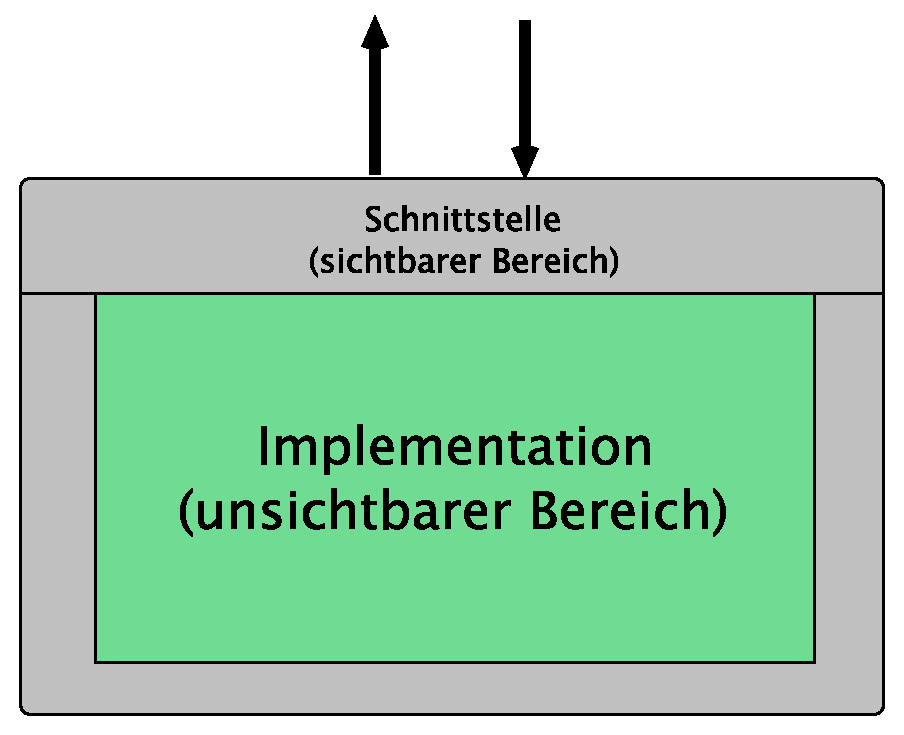
\includegraphics[width=0.6\textwidth]{material/images/simple-module.png}
        \caption{Simple Modulstruktur}
        \label{fig:simple-module}
      \end{figure} 
    Somit dient das Modul als ein Behälter für Objekte, der aus einem unsichtbaren und einem sichtbaren Bereich besteht. Der sichtbare Bereich ist die Schnittstelle des Moduls und ist die Aufzählung derer Objekte, die das Modul nach außen hin zur Verfügung stellt. Der Zugriff auf diese erfolgt über definierte Operationen in der Modulschnittstelle. 
    Der unsichtbare Teil beherbergt die eigentliche Implementierung, also die umgesetzten Operationen und Daten.
    Uner diesen Umständen reduziert sich die Komplexität des Moduls für den Nutzer von der Gesamtimplementation auf die Schnittstellen. 
      \begin{figure}[h!]
        \centering
        \includegraphics[width=\textwidth]{material/images/module-workflow.png}
        \caption{Schematischer Aufbau eines Moduls}
        \label{fig:module-workflow}
      \end{figure} 
    \newline In der Abbildung \ref{fig:module-workflow} wird die interne Struktur sowie entsprechenden Verbindungen eines Moduls genau betrachtet. Zu sehen sind drei Module, die ihre Dienste mit dem \textit{export} Schlüssel über die Schnittstellen anbieten und diese bei Bedarf mit anderen Modulen kombinieren können, indem weitere Funktionalität durch den \textit{import} Schlüssel von zusätzlichen Modulen angefordert wird. Die interne Umsetzung der Funktionalität bleibt jedoch verborgen und kann Modulübergreifend nicht nachverfolgt werden. 

  % Moduldefenition schlussatz als zusammenfassung 
  \subsection{Moduldefinition}
    \begin{itemize}
      \item Zusammenfassung von Operationen und Daten zur Realisierung einer in sich abgeschlossenen Aufgabe 
      \item Kommunikation mit der Außenwelt nur über eine eindeutig spezifizierte Schnittstelle 
      \item Nutzung des Moduls möglich ohne Kenntnis des inneren Ablaufs 
      \item Die Struktur jedes Moduls sollte einfach genug sein, um vollständig verstanden zu werden.
      \item Anpassungen eines Moduls sollte ohne Kenntnis der Implementierung sowie ohne Einfluss auf das Verhalten anderer Module durchführbar sein.
      \item Korrektheit des Moduls durch Tests nachprüfbar ohne Kenntnis seiner Einbettung
      \item Wiederverwendbarkeit der Funktionalität im anderen Kontext
    \end{itemize}

  % Wie modelliert man Module  
  \subsection{Modulentwurfskriterien}
    % Einleitung
    Nachdem die Struktur des Moduls klar bestimmt wurde, muss die Umsetzung einer Applikation mit Modulen auf Qualitätsmerkmale abgeglichen werden. 
    Da die Aufteilung eines Entwurfsproblems in kleinere Teilprobleme nicht Selbstverständlich ist, kann diese mit verschieden Techniken und auf diverse Weise umgesetzt werden und bietet daher keine Garantie eines sauberen Entwurfs. 
    Die Kunst Funktionalität in einem einzelnen Modul zu kapseln und diese mit geringer Abhängigkeit vom Restsystem betreiben zu können, kann mit Hilfe bestimmter Kriterien bewertet und angepasst werden.
    
    \bigbreak Bei der Modularisierung sind folgende Entwurfskriterien zu berücksichtigen: 
    \begin{itemize}
      \item Modulgeschlossenheit 
      \item Maximale Modulbindung 
      \item Minimale Modulkopplung 
      \item Minimale Schnittstelle 
      \item Modulanzahl 
      \item Modulgröße 
      \item Testbarkeit 
      \item Seiteneffektfreiheit 
      \item Importzahl 
      \item Modulhierarchie 
    \end{itemize}
    Mit Hilfe der \textit{Modulgeschlossenheit} wird die Abhängigkeit des Moduls von anderen Modulen reduziert und lässt diese separat bearbeiten und austauschen. Somit kapselt ein Modul eine bestimmte Funktionalität, die von Anfang bis zum Ende intern verarbeitet werden kann. 
    Direkt daraus folgt im besten Fall eine \textit{maximale Bindung} oder starker Zusammenhang innerhalb eines Moduls, indem die internen Komponenten bestens mit einander verzahnt sind und sich gemeinsam mit eine gezielten Aufgabe beschäftigen. In der Konsequenz entsteht ein eingeschränkter Wartungsraum für Entwickler, die sich mit der entsprechenden Funktion beschäftigen.   
    Um die Bindung der Komponenten innerhalb eines Moduls zu messen, können die Abhängigkeiten in verschieden Kategorien eingeteilt werden: Logisch, Zeitlich, Prozedural, Sequentiell, Informal und Funktional.
    \begin{figure}[h]
      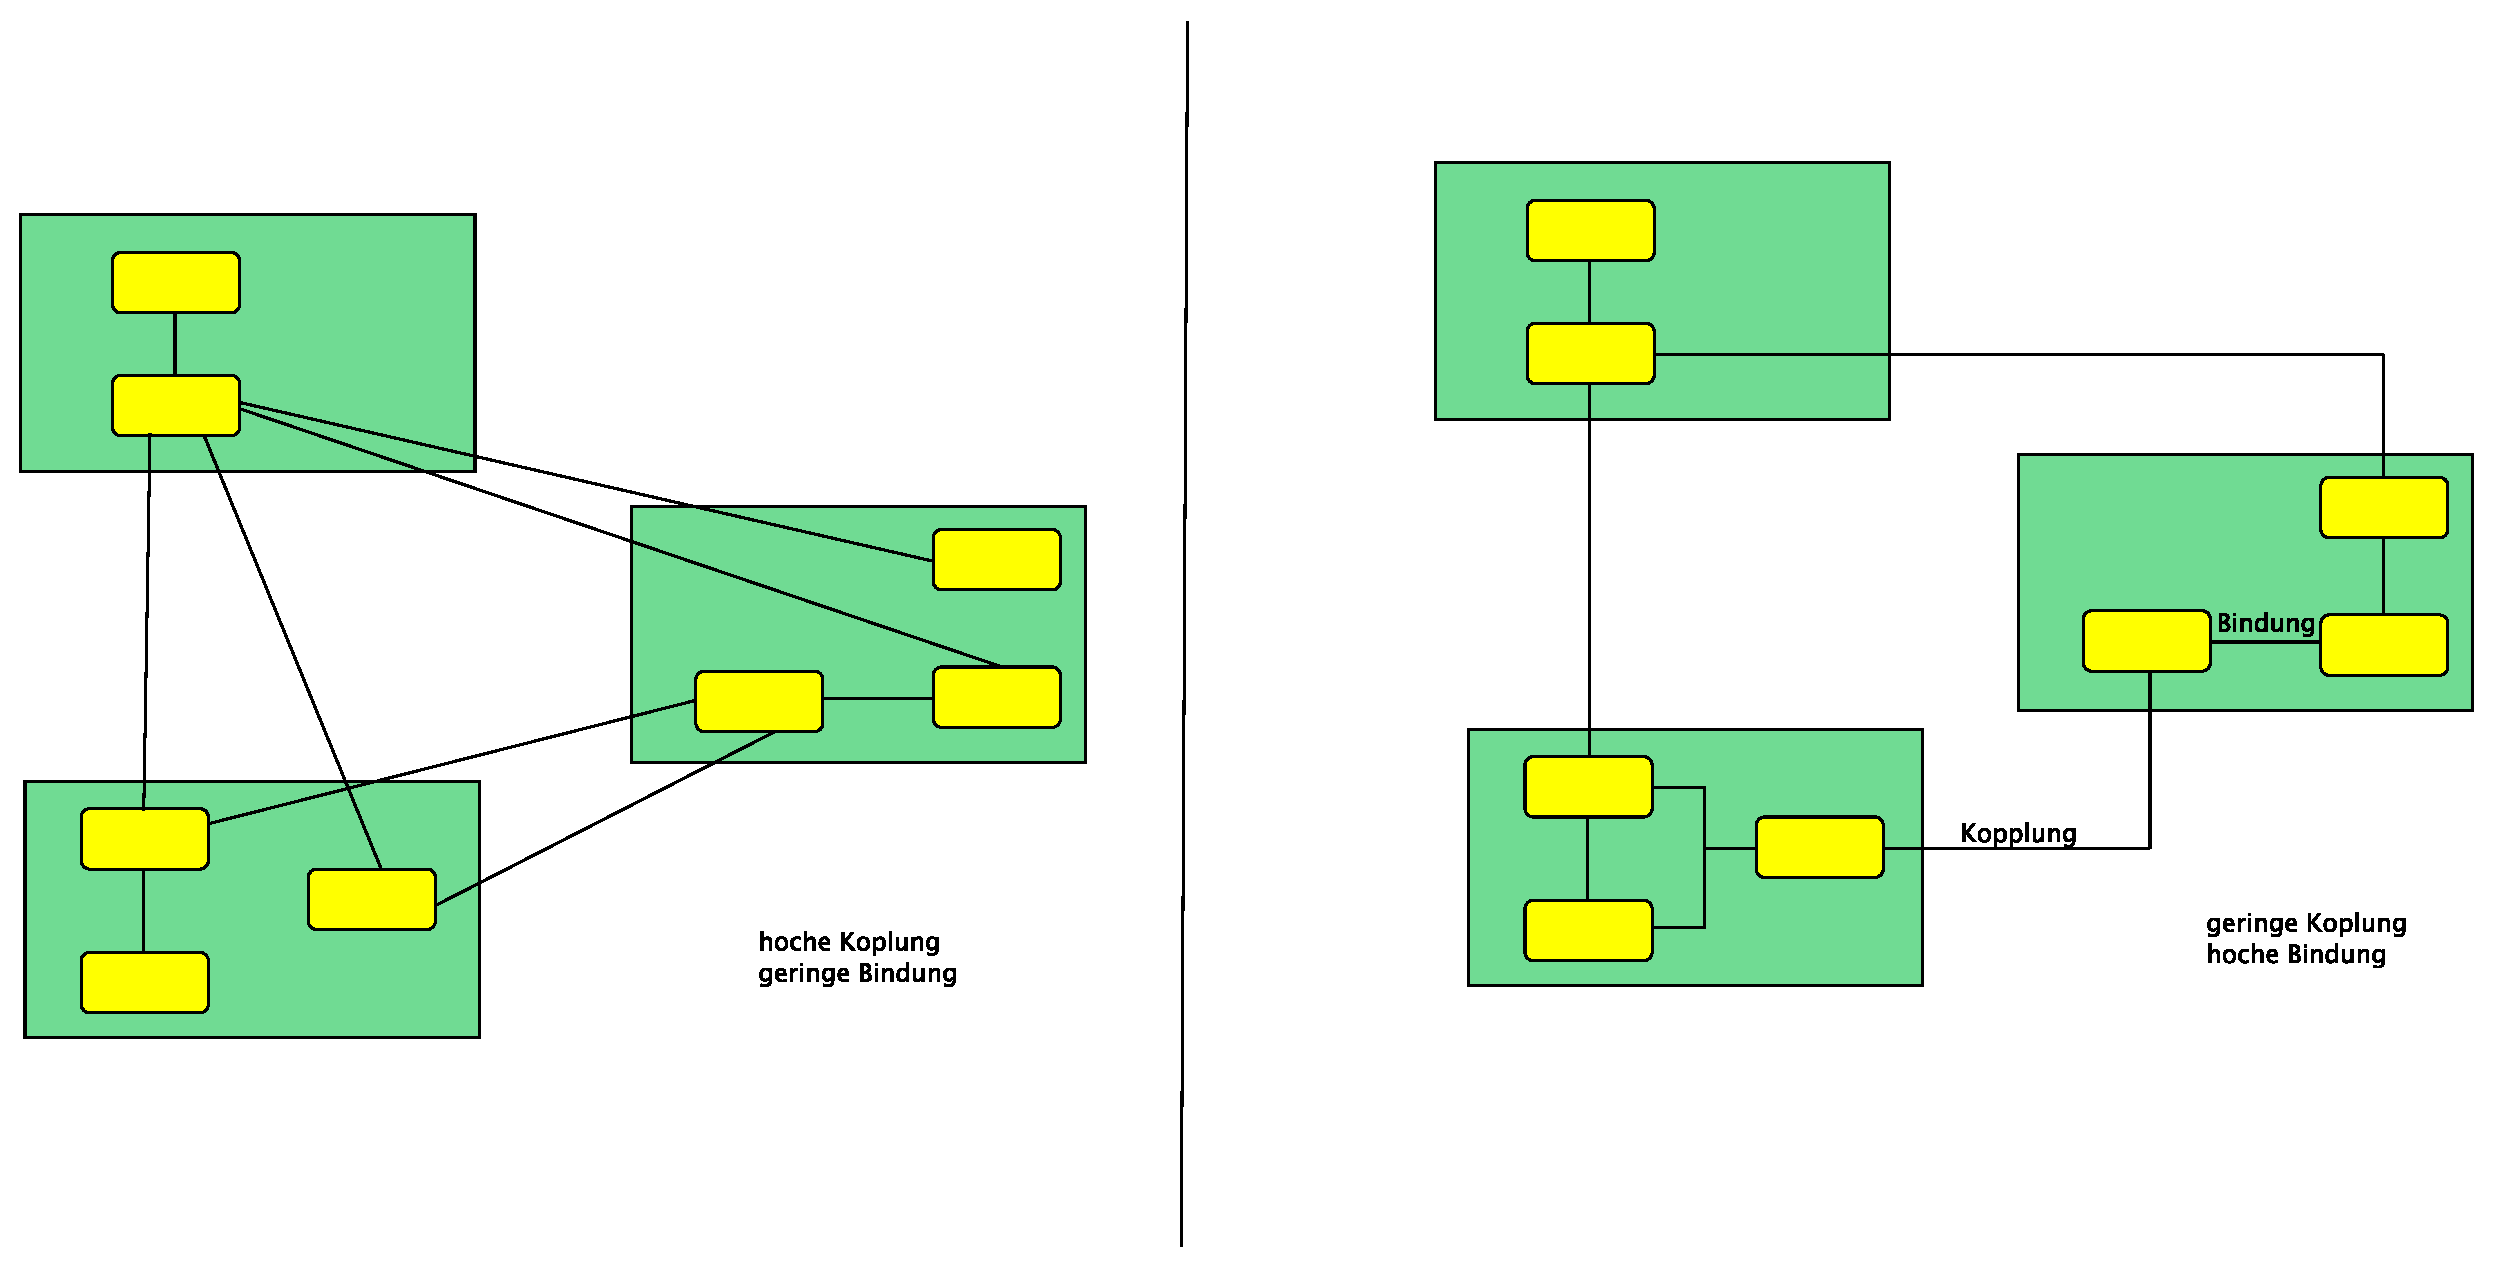
\includegraphics[width=\textwidth]{material/images/kopplung.png}
      \caption{Modulbindung und Modulkopplung}
      \label{fig:kopplung}
    \end{figure}
    \newline Komplementär zu der \textit{maximale Bindung} beschreibt die \textit{minimale Kopplung} die Anzahl der Verbindung zwischen den Modulen. Diese sollte natürlich klein gehalten werden, um die Abhängigkeit zu reduzieren. 
    Die \textit{minimale Kopplung} hat somit einen direkten und positiven Einfluss auf die Anzahl der Schnittstellen, indem diese übersichtlich und eindeutig die Funktion des Moduls beschreiben. 
    Andernfalls kann eine starke Kopplung die Komplexität heben und Fehler begünstigen, indem der Umfang an Daten, die zwischen den Modulen ausgetauscht werden, erhöht wird. 
    Eine \textit{minimale Kopplung} ist ein guter Ansatz den unnötigen Datentransfer zu reduzieren, garantiert aber keine lose Kopplung von den umgebenen Modulen. 
    Daher sollte der Begriff \textit{Seiteneffektfrei} eingeführt werdend. 
    Dieser beschreibt den Einfluss eines Moduls auf seine Umgebung, indem das Modul Unverzichtbar für die Gesamtfunktionalität wird und der Austausch die Anpassung verknüpfter Module nach sich zieht. 
    Das ist öfters der Fall wenn eine Aufgabe modulübergreifend gelöst werden muss und die Aufgabenkapslung für diesen Zweck aufgelöst wird.

    % Modularten wie Platform Explicit Modules, Application Explicit Modules, Automatic Modules, Open Modules, Unnamed Module 
  \subsection{Modularten}
    Das Modulsystem von Java unterscheidet die Module in fünf unterschiedliche Arten, diese richten sich nach der Aufgabe und ihrer Umsetzungsstruktur. 
    Zum einen gibt es die JDK \textit{Plattform Module}, die die Kernfunktionalität der Java Laufzeitumgebung bieten und bringen Pakete wie \textit{java.lang, java.io} und \textit{java.net} mit sich. 
    Andererseits gibt es die Benutzer konstruierten \textit{Applikationsmodule}, die durch eine explizite Komposition bestimmte Aufgaben erfüllen.  
    Beide Modultypen beinhalten eine \textit{Modulbeschreibung}, die dessen Abhängigkeiten und Schnittellen beschreiben. 
    \newline Obwohl mit den vorher genannten \textit{expliziten Module} Softwaresystemen realisieren lassen, fehlt die Offenheit bestimmter Module oder ihrer Pakete für die Umsetzung der Reflection Bibliotheken, die dynamischen Zugriff auf unsere Pakete während der Laufzeit benötigten. 
    Wie im Kapitel \ref{sec:reflaction} besprochen ist Reflection ein wichtiges Werkzeug in der Softwareentwicklung und wird in den neuen Java Modulsystem unterstützt. 
    Um Reflection in einem Modul zu aktivieren, reicht es lediglich das ganze Modul als \textit{open module} oder mit Hilfe des \textit{opens package.name} Schlüssels ein spezielles Paket des Moduls in der \textit{Modulbeschreibung} zu deklarieren.  
    Damit hätte man ein für Reflection offenes Modul und könnte dessen öffentlich sowie privaten Klassen dynamisch aus jedem Module auf dem Modulpfad aufrufen.
    Da diese Module das Konzept der starken Kapselung aufgeben, werden diese zu einem besonderen Typen der \textit{offenen Module} zugeordnet.
    \begin{figure}[h]
      \centering
      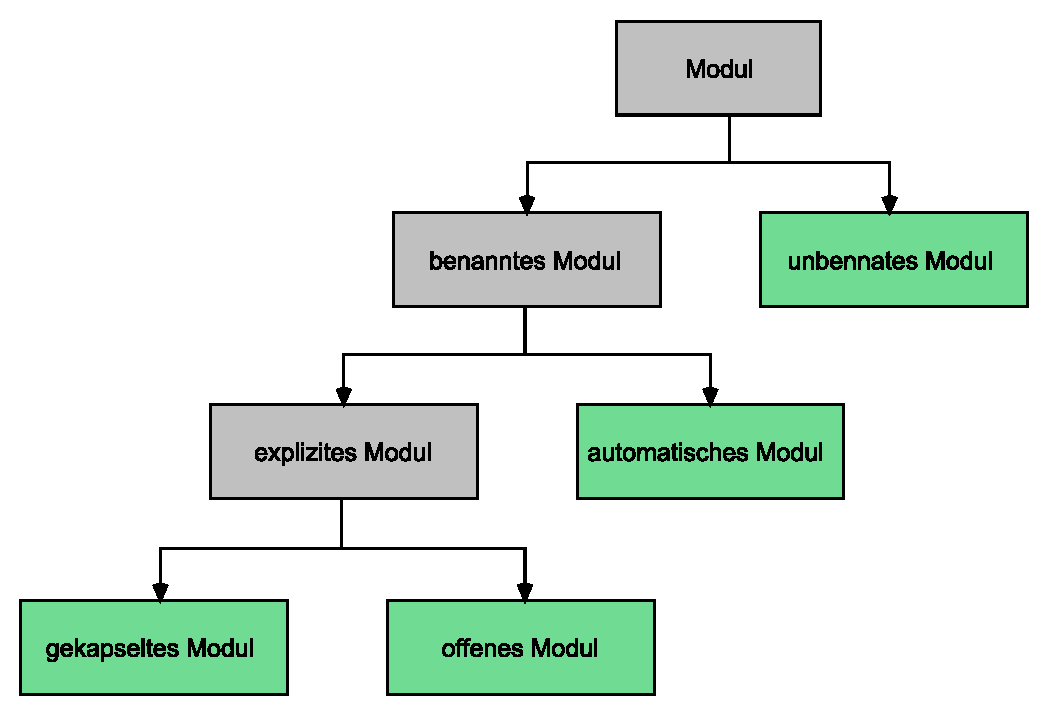
\includegraphics[width=0.7\textwidth]{material/images/module-tree.png}
      \caption{Modularten}
      \label{fig:kopplung}
    \end{figure}
    \newline Die nachfolgenden Modultypen sind Pseudo-Module, die für die Unterstützung der Abwärtskompatibilität eingeführt worden sind. 
    Dementsprechend sollen diese Module eine Brücke zwischen existierender Applikation und der modularisierten Architektur bilden. 
    \newline Das \textit{unbenannte Modul} beschreibt alle Klassen und JAR's, die sich parallel zu der Codebasis des Modulpfades auf dem Klassenpfad befinden. 
    Das \textit{unbekannte Modul} beschreibt somit die Legacy-Teil der Codebasis, die noch Migriert werden muss und es noch nicht tun kann.
    Daher wird mit der Bezeichnung \textit{unbekanntes Modul} eine Zugriffsbarriere zwischen der modularisierten und der legacy Architektur errichtet, die die \textit{expliziten Module} vom Zugriff auf den veralteten Klassenpfad abgrenzt. 
    Denn dieses trägt keinen Namen und kann somit vom Entwickler nicht Pragmatisch referenziert werden. 
    \newline In folge dessen entstehen eine asymmetrische Kommunikation zwischen den Architekturen. 
    Die \textit{expliziten Module} arbeiten nur auf dem Modulpfad im neuen System und das \textit{unbekannte Module} darf zusätzlich zu den klassischen Klassenpfad auf den modernen Modulpfad zugreifen. 
    Diese Umsetzung lässt eine inkrementelle Migration der Codebasis auf das Modulsystem zu und bleibt Lauffähig, obwohl die Applikation eine interne Versionsdiskrepanz beinhaltet.
    \begin{figure}[h]
      \centering
      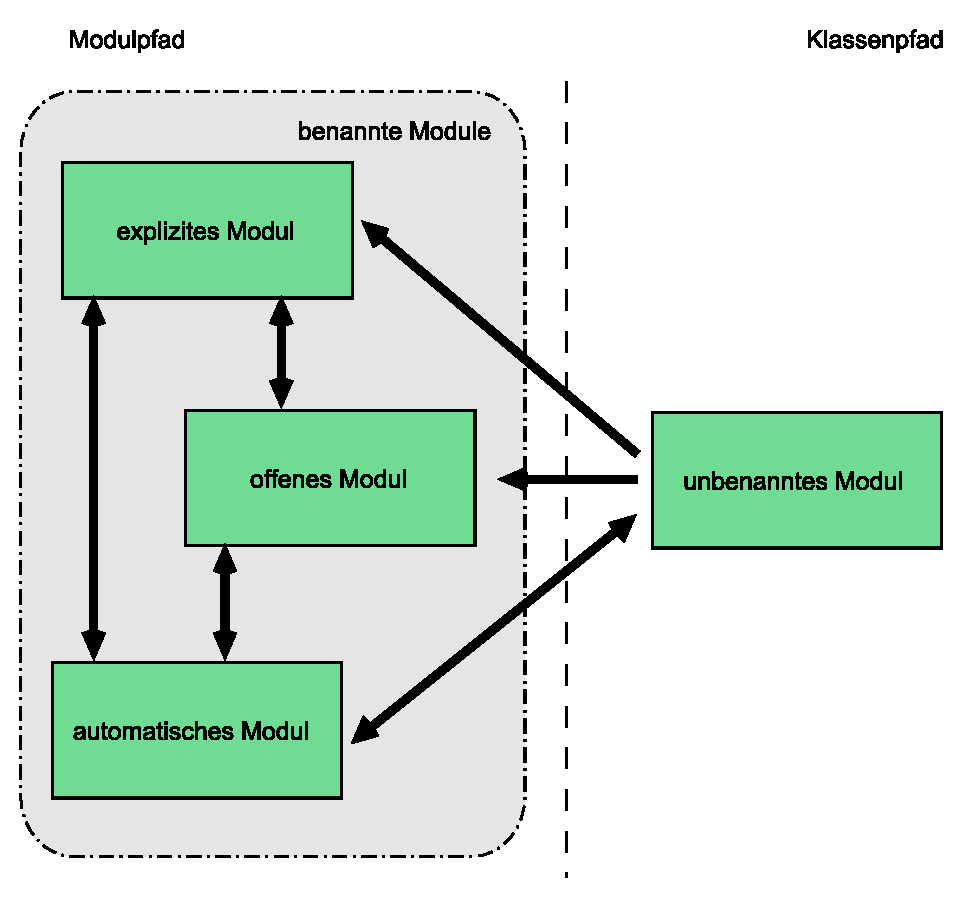
\includegraphics[width=0.7\textwidth]{material/images/module-access.png}
      \caption{Modulzugriffsrechte}
      \label{fig:kopplung}
    \end{figure}
    \newline Das letzte Modul beschreibt ein Modul mit speziellen Verhalt, das sich zwischen den Architekturen stellt und eine Brücke zwischen den Modulpfad und Klassenpfad errichtet.
    Das \textit{automatischen Module} beschreiben einen Migrationsansatz der bestehenden Bibliotheken, die vom Klassenpfad auf den Modulpfad verschoben werden und keine \textit{Modulbeschreibung} besitzen. 
    Diese kriegen einen Modulnamen zugewiesen und könne über diesen von den \textit{expliziten Modulen} aufgerufen werden. 
    Somit übernimmt Java die Kopplung der \textit{automatischen Modulen} mit allen \textit{expliziten Modulen}, indem alle internen Pakete für die Nutzung offen gelegt werden und alle Module auf dem Modulpfad für die Verwendung importiert werden.
    Somit ist eine Legacy-Bibliothek auf den Modulpfad funktionstüchtig und bietet eine ganz besondere Fähigkeit, nämlich den Zugriff auf dessen Funktionalität aus dem Modulpfad sowie den Klassenpfad. 
    Dank dieser Fähigkeit können Bibliotheken migriert werden und beide Architekturen zu gleich unterstützen. 
    Dieses Verhalten fördert die Entwickler ihren Code für den Modulpfad zu entwickeln, da die nötigen Legacy-Bibliothek der Applikation in beiden Architekturen zugleich verfügbar sind. 
    Dennoch schafft das \textit{automatischen Module} zusätzliche Komplexität in die Architektur, indem 
    alle Module mit diesem verbunden werden. Daraus folgt eine starke Kopplung und somit eine unübersichtliche, starke Abhängigkeit zwischen den Modulen.
    \newline Nichtsdestotrotz bieten automatischen und den unbenannten Modulen diverse Migrationsszenarien, die flexible Wege für die Modernisierung der Applikation anbieten. 

  

 
\subsection{Modulkopplung}
		

Die Einführung des Modulsystems in Java 9 trug im Kern das Konzept der Aufteilung einer monolithischen Umsetzung in übersichtliche mit einender sachlich verbunden Modulen. 
Dieses sollte von Java selbst ausgehen und ihre eignen sowie darauf aufbauenden Code Umstrukturieren.
In der praktischen Umsetzung sind die Schnittstellen durch die \textit{module-info.java} formuliert und enthält drei Kopplungsarten: Durch die \textit{require, export} und \textit{open} Schlüssel, die ferner konfiguriert werden können. 
! Bild java-info.java
- Beschreibung der Erweiterungen von den drei Verbindungen und ihren Nutzen in einem Listenformat.
  - transitiv
  - opens
  - requires
  - static
  - uses
  - provides 
! Bild Abhängigkeitsgraph
-  Beschreibe das es hier um Zugriffsrechte geht 

- Dementsprechend dienen die Kopplungsschlüssel nicht nur der Lesbarkeit, sondern erweitern die Prozedur des Klassenladens durch explizite Zugriffsberechtigungen. 
- Java 9 besitzt immer noch die Klassloader Hierarchie mit den Boot-,dem umbenannten Plattform und Applikationsloader.
- In den modernisierten JDK  übernehmen sie das laden bestimmter Module anstelle der ehemaligen JAR's.
!  <bild oder Tabelle unterteilt Module auf die drei  Klassloader> 
- Rückblick auf classpath Kapitel 
- Java 9 wurde modularisiert und hat es vorgezeigt, indem der JDk modularisiert wurde und mit Hilfe eines Abhängigkeitsgraphen  die nötigen KModule in die Applikation eingebunden werden können. Diese könne direkte, transitive oder offenen Verbindungen beinhalten. Wichtige Eigenschaft des Modularen Ansatzes ist die Struktur des Abhängigkeiten darf nicht in einem Kreis enden.
! <hier ist ein Bild wie ein Azyklischer Modulgraph aussehen könnte.> 
- Schlusssatz 


% vergleich  mit existierenden Umsetzungen
\newpage \subsection{Vergleich Konzeptumsetzungen}
  Im folgenden Kapitel vergleiche JPMS mit anderen Modularisierungstechniken und betrachten deren Gemeinsamkeiten, Unterschiede und Möglichkeiten der Kombination. 

% Product no Project
\subsubsection{Mikroservices}
  Mikroservices ist eine Architekturstil mit einer große Menge an Designmuster und -prinzipien, die sich Industrieweit durchgesetzt haben und alle möglichen Sprachen sowie Komponenten zusammenbringen. 
  Diese beschäftigen sich mit der Aufteilung einer großen, monolithischen Applikation in kleinere, lose gekoppelte Komponenten, die über das Netzwerk kommunizieren und als ein ganzes Produkt abgestimmt werden.
  Infolge dessen entstehen modulare Systeme mit den dazugehörigen Vorteilen und kann aus diesem Grund für viele Anwendungen anstelle der \textit{Java Plattform Module System} genutzt werden.
  Dennoch haben Mikroservices ihre Nachteile, denn sie betreiben die Module in einem verteilten System über das Netzwerk mit den entsprechenden Schwachstellen und Schattenseiten.
  \bigbreak Der große Unterschied zwischen Mikroservices und JPMS liegt in der Zielsetzung und Umsetzungsschicht der Module. 
  Da Mikroservices Module, von Oben nach Unten, auf der Architekturebene entwerfen und diese nach ihrer eigener Weltanschauung umsetzen, beschäftigt sich JPMS im Gegensatz dazu mit der bewussten Softwareentwicklung auf der Sprachebenen und modelliert Klassen-, Paketen- und Module von Unten nach Oben auf.
  Ein weiterer unterschied liegt im Betrieb der Module, denn für den Betrieb der JPMS Applikation müssen alle Module in ihrer Gesamtheit deployed werden und von außen betrachtet nur als eine einzelne Einheit wahrnehmbar sein. 
  Mikroservices hingegen werden als klar getrennte Module auch während des Betriebs wahrgenommen. 
  Infolgedessen adressierten Mikroservices Probleme über die JPMS keine Meinung hat, wie zum Beispiel \textit{Islands of functionality, Lightweight protocols} oder \textit{Graceful error handling} \ref{tab:jpms}. Somit überschneiden sich die beiden Umsetzungen in ihrer Zielsetzung, jedoch tun sie es in unterschiedlichen Kompetenzbereichen.  
  \bigbreak Nichtsdestotrotz können sich die beide Ansetze ergänzen, indem JPMS auf der Implementierungsebene die Codestruktur Modular gestalten, die anschließend mit einer Mikroservices Architektur als Services distributiv aufgesetzt wird. 



  \begin{table}[h!]
      \label{tab:jpms}
      \begin{tabular}{l|l}
        \textbf{Mikroservices} & \textbf{JPMS}\\
        \hline
        Architekturstil & Klassen- und Prozessebene \\
        & Modularität ist integriert \\
        & Modularität ist Kern der Plattform \\
        \hline
        Evolutionäres Design  & Bewusste Softwareentwicklung \\
        Unabhängiges Deployment &\\
        Überwachbar &\\
        Ersetzbar &\\
        \hline
        Technologische Entkoppelung & - \\
        Kleine Komponenten &\\ 
        Isolierte Funktionsinseln &\\
        Leichte Kommunikationsprotokolle&\\
        Geschickte Fehlerbehandlung&\\

      \end{tabular}
      \caption{Gegenüberstellung von Mikroservices und JPMS}
  \end{table}


\subsubsection{OSGi}


\subsubsection{Docker}
\subsubsection{JavaScript}
\subsubsection{TypeScript}
\subsection{Java Umsetzung} 
% wie es war mit 1.8
% was draus gewirden ist in 9
\newpage

\section{Vergleich mit anderen Modularisierungskonzepten}


\subsection{Jigsaw}
% wie löst java 9 die Probleme 
% theoretisch 
\subsection{Modular JDK}
% bevor entwickler modularisieren muss da System selbst modular sein.
% eine beispiel umsetzung
% löst probleme von beginn an, praktische umsetzung 
\subsection{Modulstruktur}
% arten von modulen 
% inhalt und aufbau
% zugriffsberechtigungen 
\subsection{Modulepfad}
% classloader änderungen 
% verweist nicht mehr auf klassen orte sondern auf  modul Orte
\subsection{Optionale Abhängigkeiten}
%  optionale erweiterbarkeit
\subsection{Reflection}
%  sicherer und braucht explizite konfiguration 
% zugriff auf  alle klassen nicht mehr möglich 
\subsection{Services} 
\subsection{Migration}

\section{Vergleich mit anderen Modularisierungskonzepten}


\section{Modularisierungskonzepten}

\subsection{Java Plattform Module System}

\subsection{Vergleich mit anderen Modularisierungskonzepten}

\subsection{Vom Classpath zum Modulpath}

\subsection{Arten von Jigsaw-Modulen}

\subsection{Service-Provider und -Consumer}

\subsection{Abhängigkeitsgraph mit Graphviz}


- Module gabs schon lagne 
- osg 
- und und und 
- angular 
\chapter{Modularisierung} \label{cha:modularisierung}

% \section{Modularisierung} \label{sec:modularisierung}
  Modularisierungsansätze finden sich so gut wie in jeder Software wieder, da es sich um ein grundlegendes Prinzip für die Beherrschung eines Systems handelt. Gerade in der Java-Welt wird seit jeher das Ideal von lose gekoppelten Systemen verfolgt, denn diese generieren die Struktur in großen Softwareprojekten, indem das Gesamtprodukt in kleine und praktische Bestandteile zerlegt wird. \bigbreak
  
  Die Entwicklung von kleinen Projekten mit einer übersichtlichen Codebasis ist einfach zu überblicken und bedarf keiner strukturellen Unterstützung, um den Entwickler, Architektur und Funktion darzustellen. Dennoch ist die Zukunft eines Projekts nicht immer eindeutig und kann mit der Zeit an Größe und Komplexität gewinnen. Mit der Größe des Projektes, wächst der Geschäftskontext und damit die Zahl der beteiligten Personen. Diese repräsentieren verzwickte Wünsche und Ziele, die an einer Stelle im Projekt nicht sauber umsetzbar sind. Infolge dessen ist die richtige Aufstellung eines Projektes von Grund auf eine zukunftssichere Entscheidung.\bigbreak 

  Ohne die Modularisierung werden Änderungen an großen Projekten mühselig und mit unerwarteten Nebeneffekten umgesetzt. Sowohl das Bauen und Ausrollen des Projekts, als auch der Betrieb der Applikation, ist eine lange und aufwendige Aufgabe, die mit jedem kleinen Fehler die komplett Applikation neustarten lässt oder das Ausrollen unterbricht. Somit können kleine Fehler das ganze Produkt aus dem Gleichgewicht bringen. Aus diesem Grund sollen Module diese Probleme adressieren und die Applikation in autonome, kleine Einheiten aufteilen, die unabhängig voneinander ihre Funktionalität anbieten.

  % Moduleigenschaften 
  \section{Ziele der Modularisierung} \label{sec:ZdM}
    Die Modularisierung beschäftigt sich mit der Aufteilung eines Systems in Module, die Komplexität verringern, indem die einzelnen Module getrennt voneinander betrachtet und verstanden werden. Dies wiederum unterstützt die Wartbarkeit der einzelnen Module. Darüber hinaus vereinfachen die von der Modularität geforderte Schnittstellenspezifizierung die Kommunikation zwischen den Modulen und fördert damit die Erweiterbarkeit des Systems. Da die Module austauschbar sind und unabhängig voneinander betrieben werden können, eröffnen sich neue Möglichkeiten der Softwareentwicklung. Wie zum Beispiel die Erstellung verschiedenen Varianten der Umsetzung, durch die Rekombination existierender Module, ohne die ganze Applikation zu in Betracht zu ziehen.\cite{javaMod9,java9modRevealed,explorJava9}\bigbreak

    Um die Aufgabe der Java Modularisierung zu verstehen, bedarf es einer Aufstellung von Zielen und Qualitäten, denen sich die Modularisierung stellt. Für JPMS sind diese eindeutig in der \textit{JSR 376} \cite{jmsOracle,java9modRevealed} beschrieben und spezifizieren die folgenden Qualitäten:

    \subsubsection{Kapselung}
      Die Kapselung beschreibt ein Kontrollmechanismus, der die interne Struktur eines Moduls verwaltet. Demzufolge hat das Modul die komplette Kontrolle über ihre interne Struktur und kennt die Zugriffsrechte ihrer Bestandsteile, indem das Modul die Zugriffsrechte ihrer inneren Struktur explizit deklariert.

    \subsubsection{Interoperabilität}
      Die Interoperabilität beschreibt die Kommunikationsfähigkeit der Software mit anderen diversen Systemen, unabhängig von ihrer Sprache oder Plattform. Darum bieten Module Schnittstellen an, mit denen sie Dienste anbieten und anfordern können.

    \subsubsection{Zusammensetzbarkeit}
      Aus der Interoperabilität geht die Zusammensetzbarkeit hervor. Diese steht für die Wiederverwendbarkeit der abgeschlossenen Module, die auf bestimmte Art und Weise kombiniert, und für unterschiedliche Zwecke in unterschiedlichen Systemen, eingesetzt werden können.

    \subsubsection{Erweiterbarkeit}
     Die Erweiterbarkeit hilft den modularen und zusammengesetzten Systems ihre Funktionalität zu skalieren, indem die Software durch individuelle Einheiten ergänzt werden kann. 

    \subsubsection{Autonomie}
      Mit der Autonomie werden unnötige Abhängigkeiten aufgelöst und nur die nötige Funktionalität für die entsprechende Aufgabe in einem Modul abgelegt. Somit können einzelne Module im Betrieb auch dann bleiben, wenn Teile des Systems nicht reagieren.

  % Modulaufbau 
  \section{Grobe Modulstruktur}
      Die zuvor aufgeführten Ziele der Modularisierung liefern bereits eine Vorstellung der Modulanforderungen.
        \begin{figure}[h!] 
        \centering
        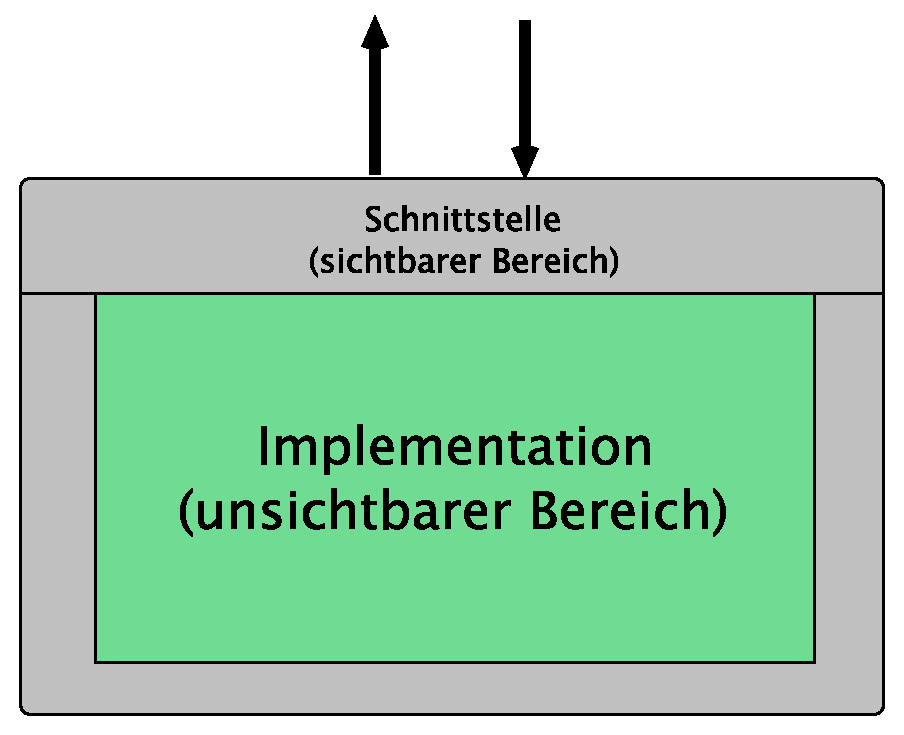
\includegraphics[width=0.4\textwidth]{material/images/simple-module.pdf}
        \caption{Simple Modulstruktur \cite{modulMitJava9}}
        \label{fig:simple-module}
      \end{figure}
    Primär erfüllt ein Modul einen abgeschlossenen Aufgabenbereich und beinhaltet die dafür nötigen öffentlichen, sowie privaten Operationen und Datenfelder. Die Kommunikation eines Moduls mit anderen Modulen und der Außenwelt, erfolgt über eindeutig spezifizierte Schnittstellen \ref{fig:simple-module}.\newline
    Somit dient das Modul als ein Behälter für Objekte, der aus einem unsichtbaren und einem sichtbaren Bereich besteht(grau und grün in der Abbildung \ref{fig:simple-module}). Der sichtbare Bereich ist die Schnittstelle des Moduls, und ist die Aufzählung derer Objekte, die das Modul nach außen hin zur Verfügung stellt. Der Zugriff auf diese erfolgt über definierte Operationen in der Modulschnittstelle. Der unsichtbare Teil beherbergt die eigentliche Implementierung, also die umgesetzten Operationen und die Daten. Unter diesen Umständen reduziert sich die Komplexität des Moduls von der gesamten Implementation auf die Schnittstellen für den Nutzer. \cite{javaMod9,java9modRevealed,explorJava9,modulMitJav9}

      \begin{figure}[h!]
        \centering
        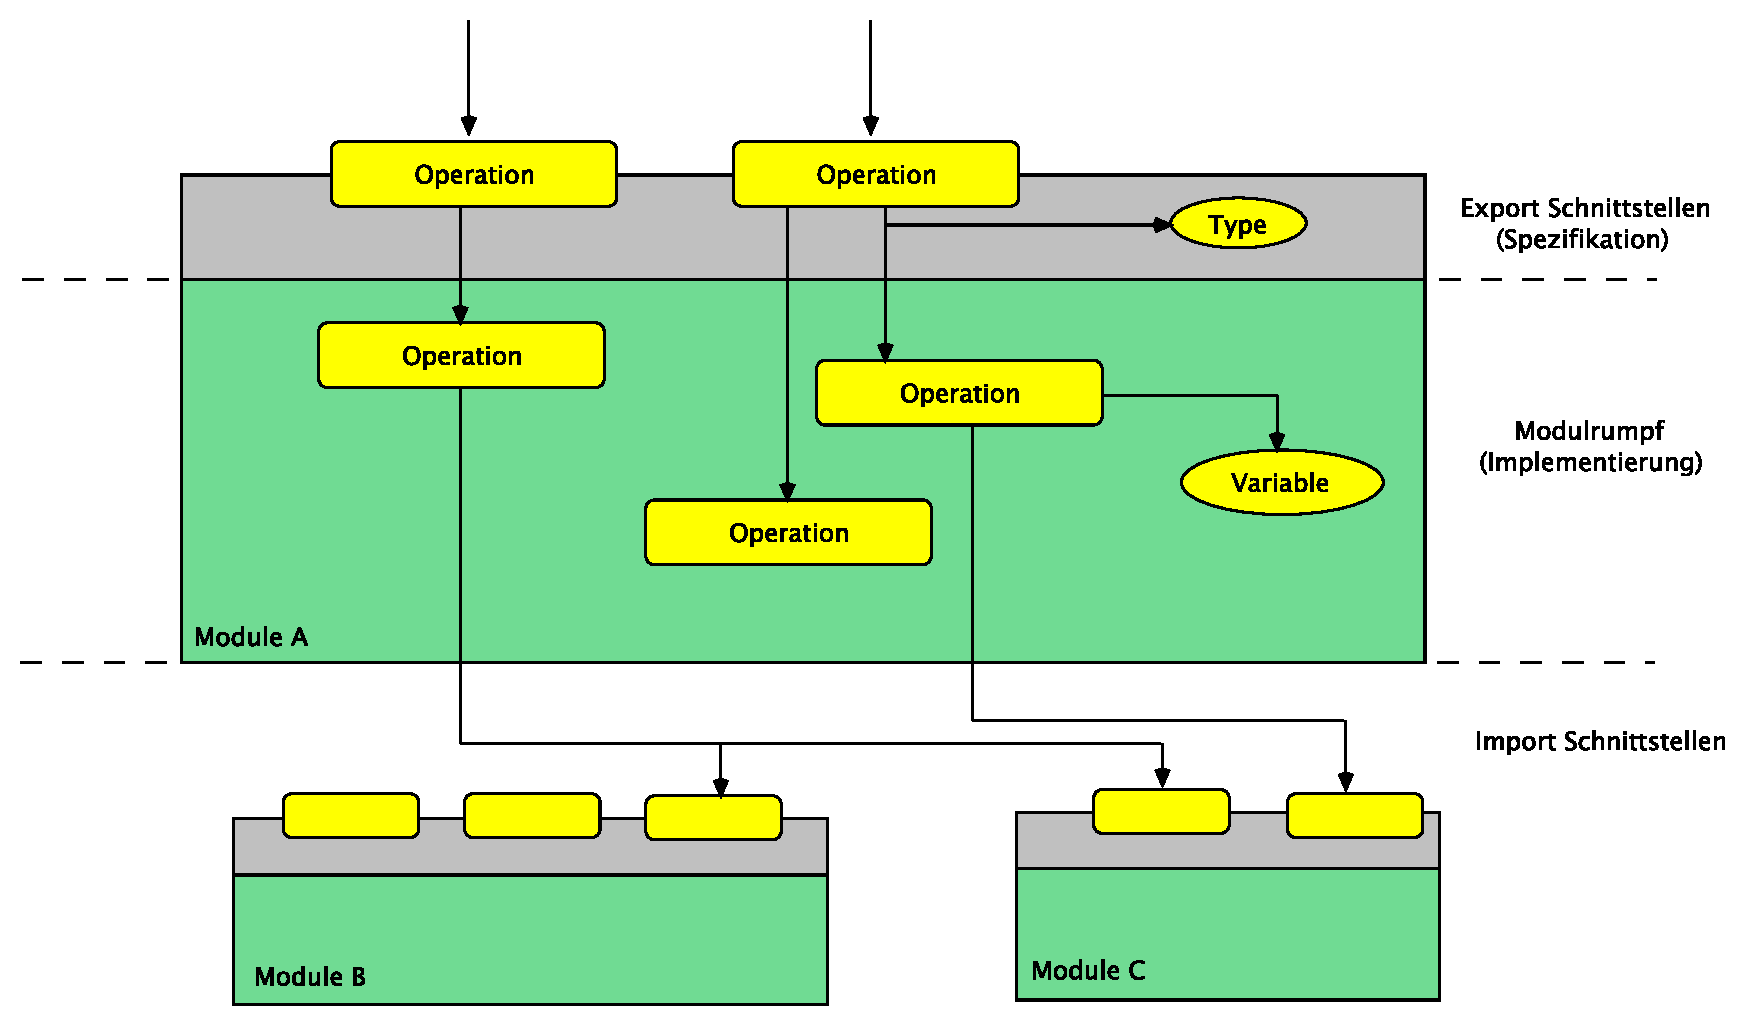
\includegraphics[width=\textwidth]{material/images/Module-workflow.pdf}
        \caption{Schematischer Aufbau eines Moduls \cite{modulMitJava9}}
        \label{fig:mw}
      \end{figure} 

    In der Abbildung \ref{fig:mw} werden die interne Struktur und die entsprechenden Verbindungen eines Moduls genau betrachtet. Zu sehen sind drei Module, die ihre Dienste mit dem \textit{exports} Schlüssel über die Schnittstellen anbieten und diese bei Bedarf mit anderen Modulen kombinieren können, indem weitere Funktionalitäten durch den \textit{requires} Schlüssel von zusätzlichen Modulen angefordert werden. Die interne Umsetzung der Funktionalität bleibt jedoch verborgen und kann modulübergreifend nicht nachverfolgt werden. 

  % Moduldefenition schlussatz als zusammenfassung 
  \section{Moduleigenschaften} \label{sec:ME}

    \textbf{Modul Definition: } \textit {Ein Modul ist eine Sammlung von Algorithmen und Daten bzw. Datenstrukturen zur Bearbeitung einer in sich abgeschlossenen Aufgabe. Die Verwendung des Moduls (d.h. seine Integration in ein Programm-System) erfordert keine Kenntnis seines inneren Aufbaus und der konkreten Realisierung der gekapselten Algorithmen und Daten(-strukturen). Seine Korrektheit ist ohne Kenntnis seiner Einbettung in ein bestimmtes Programm-System nachprüfbar.} \cite{rechenberg2006informatik}\bigbreak 

    Aus dieser Definition können folgende Eigenschaften abgeleitet werden, die ein Software-Modul beschreiben:

    \begin{itemize}
      \item Zusammenfassung von Operationen und Daten zur Realisierung einer in sich abgeschlossenen Aufgabe 
      \item Kommunikation mit der Außenwelt nur über eine eindeutig spezifizierte Schnittstelle 
      \item Nutzung des Moduls möglich ohne Kenntnis des möglichen Ablaufs 
      \item Die Struktur jedes Moduls sollte genug sein, um vollständig verstanden zu werden
      \item Anpassungen eines Moduls sollte ohne Kenntnis der Implementierung, sowie ohne Einfluss auf das Verhalten anderer Module durchführbar sein
      \item Korrektheit des Moduls durch Tests nachprüfbar, ohne Kenntnis seiner Einbettung
      \item Wiederverwendbarkeit der Funktionalität im anderen Kontext
    \end{itemize}

  % Wie modelliert man Module  
  \section{Modulentwurfskriterien} \label{sec:MEK}
    % Einleitung
    Nachdem die Struktur des Moduls klar bestimmt wurde, muss die Umsetzung einer Applikation mit Modulen auf Qualitätsmerkmale abgeglichen werden. Da die Aufteilung eines Entwurfsproblems in kleinere Teilprobleme nicht selbstverständlich ist, kann diese mit verschieden Techniken und auf diverse Weise umgesetzt werden und bietet daher keine Garantie eines sauberen Entwurfs. Die Möglichkeit Funktionalität in einem einzelnen Modul zu kapseln und diese mit geringer Abhängigkeit vom Restsystem betreiben zu können, kann mithilfe bestimmter Kriterien bewertet und angepasst werden. \cite{softModDes,softMdDes2,modulMitJava9,java9modRevealed,modulProgJava9}\bigbreak
    
    Bei der Modularisierung sind folgende Entwurfskriterien zu berücksichtigen: 
    \begin{itemize}
      \item Modulgeschlossenheit 
      \item Maximale Modulbindung 
      \item Minimale Modulkopplung 
      \item Minimale Schnittstelle 
      \item Modulanzahl 
      \item Modulgröße 
      \item Testbarkeit 
      \item Seiteneffektfreiheit 
      \item Importzahl 
      \item Modulhierarchie 
    \end{itemize}
    Mithilfe der \textit{Modulgeschlossenheit} wird die Abhängigkeit des Moduls von anderen Modulen reduziert und lässt diese separat bearbeiten und austauschen. Somit kapselt ein Modul eine bestimmte Funktionalität, die von Anfang bis zum Ende, intern verarbeitet werden kann. Direkt daraus folgt im besten Fall eine \textit{maximale Bindung}, oder ein starker Zusammenhang innerhalb eines Moduls, indem die internen Komponenten bestens miteinander verzahnt sind und sich gemeinsam mit einer gezielten Aufgabe beschäftigen. In der Konsequenz, entsteht ein eingeschränkter Wartungsraum für Entwickler, die sich mit der entsprechenden Funktion beschäftigen. Um die Bindung der Komponenten innerhalb eines Moduls zu messen, können die Abhängigkeiten in verschieden Kategorien eingeteilt werden: logisch, zeitlich, prozedural, sequentiell, informal und funktional.

    \begin{figure}[h]
      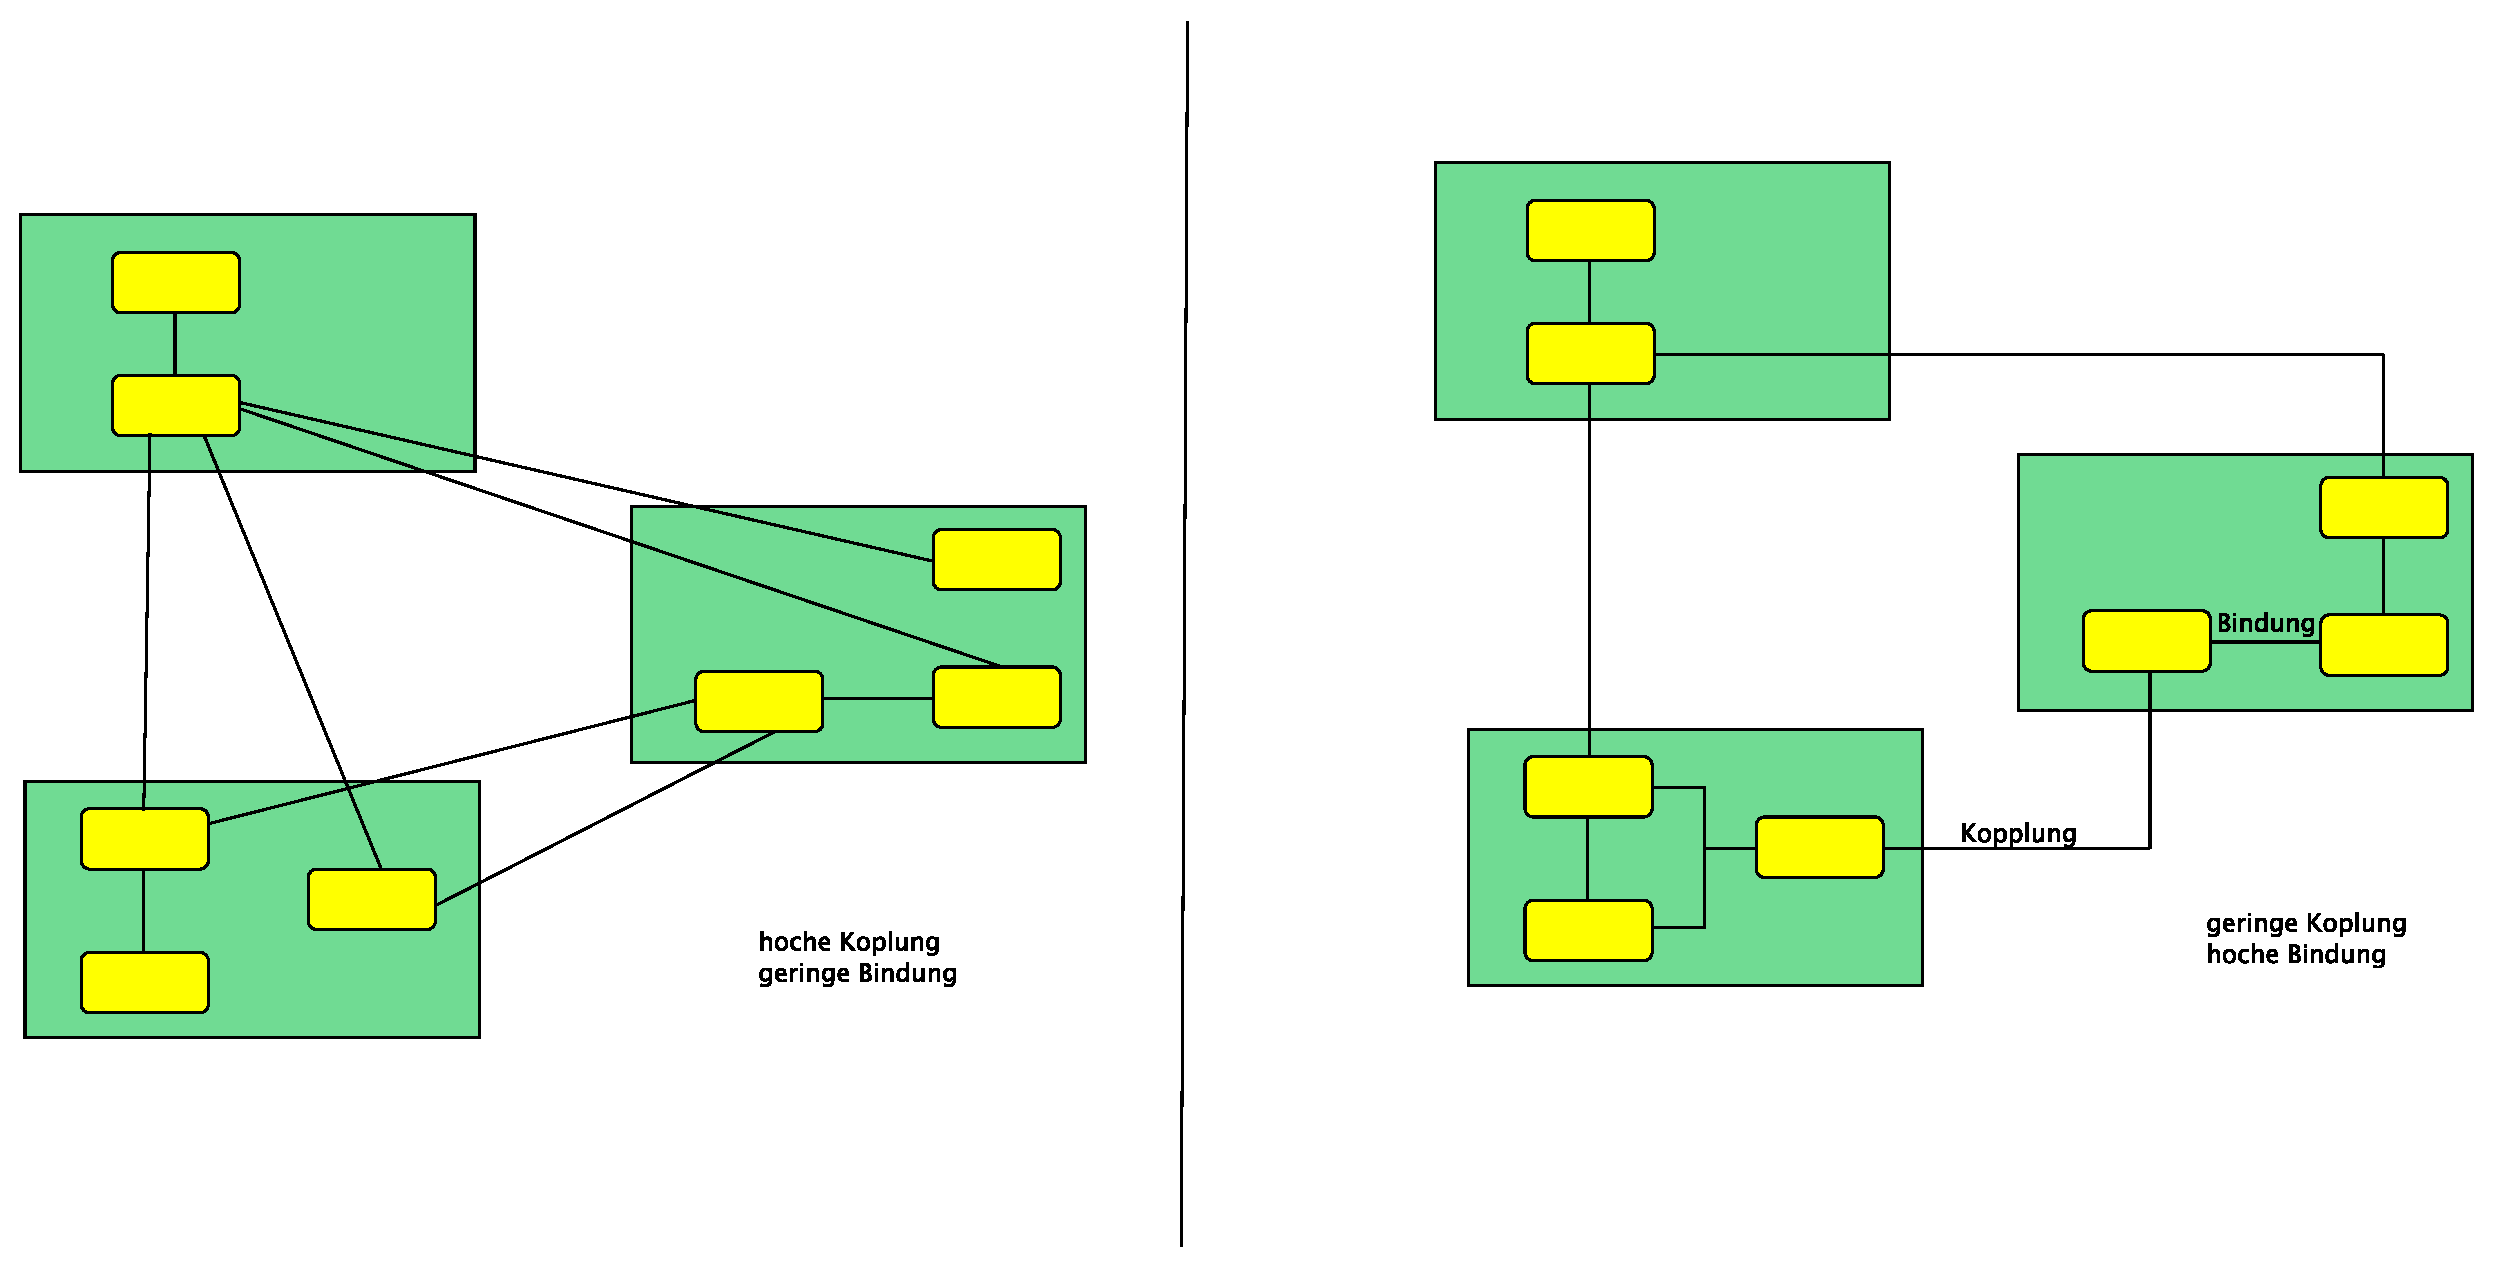
\includegraphics[width=\textwidth]{material/images/kopplung.pdf}
      \caption{Modulbindung und Modulkopplung \cite{modulMitJava9}}
      \label{fig:kopplung}
    \end{figure}

    Komplementär zu der \textit{maximalen Bindung} beschreibt die \textit{minimale Kopplung} die Anzahl der Verbindung zwischen den Modulen. Diese sollte natürlich klein gehalten werden, um die Abhängigkeit zu reduzieren. Die \textit{minimale Kopplung} hat somit einen direkten und positiven Einfluss auf die Anzahl der Schnittstellen, indem diese übersichtlich und eindeutig die Funktion des Moduls beschreiben. Andernfalls, kann eine starke Kopplung die Komplexität heben und Fehler begünstigen, indem der Umfang an Daten, die zwischen den Modulen ausgetauscht werden, erhöht wird. Eine \textit{minimale Kopplung} ist ein guter Ansatz den unnötigen Datentransfer zu reduzieren, garantiert aber keine lose Kopplung von den umgebenen Modulen. Daher sollte der Begriff \textit{Seiteneffektfrei} eingeführt werden. Dieser beschreibt den Einfluss eines Moduls auf seine Umgebung, indem das Modul unverzichtbar für die Gesamtfunktionalität wird und sein Austausch die Anpassung verknüpfter Module nach sich zieht. Das ist öfters der Fall, wenn eine Aufgabe modulübergreifend gelöst werden muss, und die Aufgabenkapslung für diesen Zweck aufgelöst wird.\cite{softModDes,softMdDes2,modulMitJava9,java9modRevealed,modulProgJava9}

    % Modularten wie Platform Explicit Modules, Application Explicit Modules, Automatic Modules, Open Modules, Unnamed Module 
  \section{Modularten} \label{Modularten}
    Das Modulsystem von Java unterscheidet die Module in fünf unterschiedliche Arten. Diese richten sich nach der Aufgabe und ihrer Umsetzungsstruktur. Zum Einen gibt es die JDK \textit{Plattform Module}, die die Kernfunktionalität der Java Laufzeitumgebung bieten, und Pakete wie \textit{java.lang, java.io}, \textit{java.net} mit sich bringen. Andererseits gibt es die Benutzer konstruierten \textit{Applikationsmodule}, die durch eine explizite Komposition bestimmte Aufgaben erfüllen. Beide Modultypen beinhalten eine \textit{Modulbeschreibung}, die dessen Abhängigkeiten und Schnittstellen beschreibt.\newline
    Obwohl sich mit den vorher genannten \textit{expliziten Modulen} Softwaresystemen realisieren lassen, müssen manche Module als \textit{offen} deklariert werden, um allen Nutzern während der Laufzeit den Zugriff auf den Inhalt zu gewährleisten und über Reflexion ihre Funktion nutzen zu können. Wie im Kapitel \ref{sec:refl} besprochen, ist Reflexion ein wichtiges Werkzeug in der Softwareentwicklung und wird in dem neuen Java Modulsystem unterstützt. Um ein ganzes Modul oder nur Teile des Moduls für Reflexion zu öffnen, kann entweder das ganze Modul als \textit{open module}, oder nur ein Paket als \textit{opens package.name} in der Modulbeschreibung deklariert werden. Damit hätte man ein für Reflexion offenes Modul und könnte dessen öffentlichen, sowie privaten Klassen, dynamisch aus jedem Modul auf dem Modulpfad aufrufen. Da diese Module das Konzept der starken Kapselung aufgeben, werden diese einem besonderen Typen der \textit{offenen Module} zugeordnet. \cite{modulMitJava9,java9modRevealed,modulProgJava9,explorJava9}

    \begin{figure}[h]
      \centering
      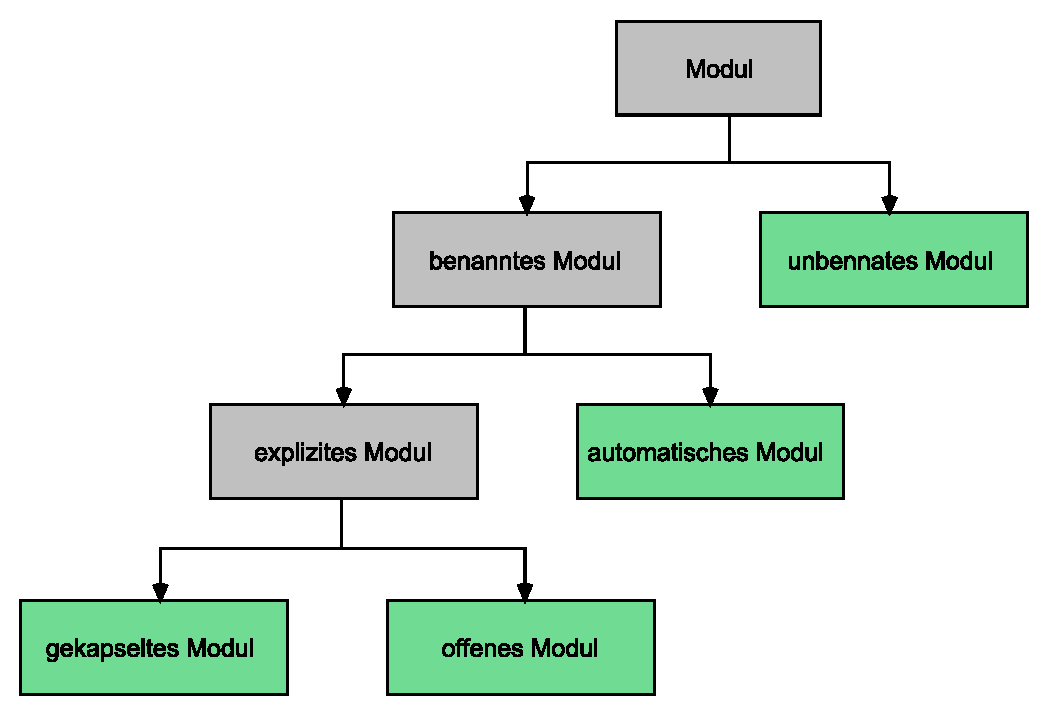
\includegraphics[width=0.7\textwidth]{material/images/module-tree.pdf}
      \caption{Modularten \cite{modulMitJava9}}
      \label{fig:modtree}
    \end{figure}

    Die nachfolgenden Modultypen sind Pseudo-Module, die für die Unterstützung der Abwärtskompatibilität eingeführt worden sind. Dementsprechend sollen diese Module eine Brücke zwischen existierender Applikation und der modularisierten Architektur bilden.\bigbreak

    Das \textit{unbenannte Modul} beschreibt alle Klassen und JAR's, die sich parallel zu der Codebasis des Modulpfades auf dem Klassenpfad befinden. Das \textit{unbenannte Modul} beschreibt somit den Legacy-Teil der Codebasis, die noch migriert werden muss, da es dies noch nicht tun kann. Daher wird mit der Bezeichnung \textit{unbenanntes Modul} eine Zugriffsbarriere zwischen der modularisierten und der legacy Architektur errichtet, die die \textit{expliziten Module} vom Zugriff auf den veralteten Klassenpfad abgrenzt. Denn dieses trägt keinen Namen und kann somit vom Entwickler nicht pragmatisch referenziert werden.\newline
    Infolgedessen entsteht eine asymmetrische Kommunikation zwischen den Architekturen. Die \textit{expliziten Module} arbeiten im neuen System auf dem Modulpfad und das \textit{unbenannte Module} darf zusätzlich neben dem klassischem Klassenpfad, ebenso auf den modernen Modulpfad zugreifen. Diese Umsetzung lässt eine inkrementelle Migration der Codebasis auf das Modulsystem zu und bleibt lauffähig, obwohl die Applikation eine interne Versionsdiskrepanz beinhaltet. \cite{modulMitJava9,java9modRevealed,modulProgJava9}

    \begin{figure}[h]
      \centering
      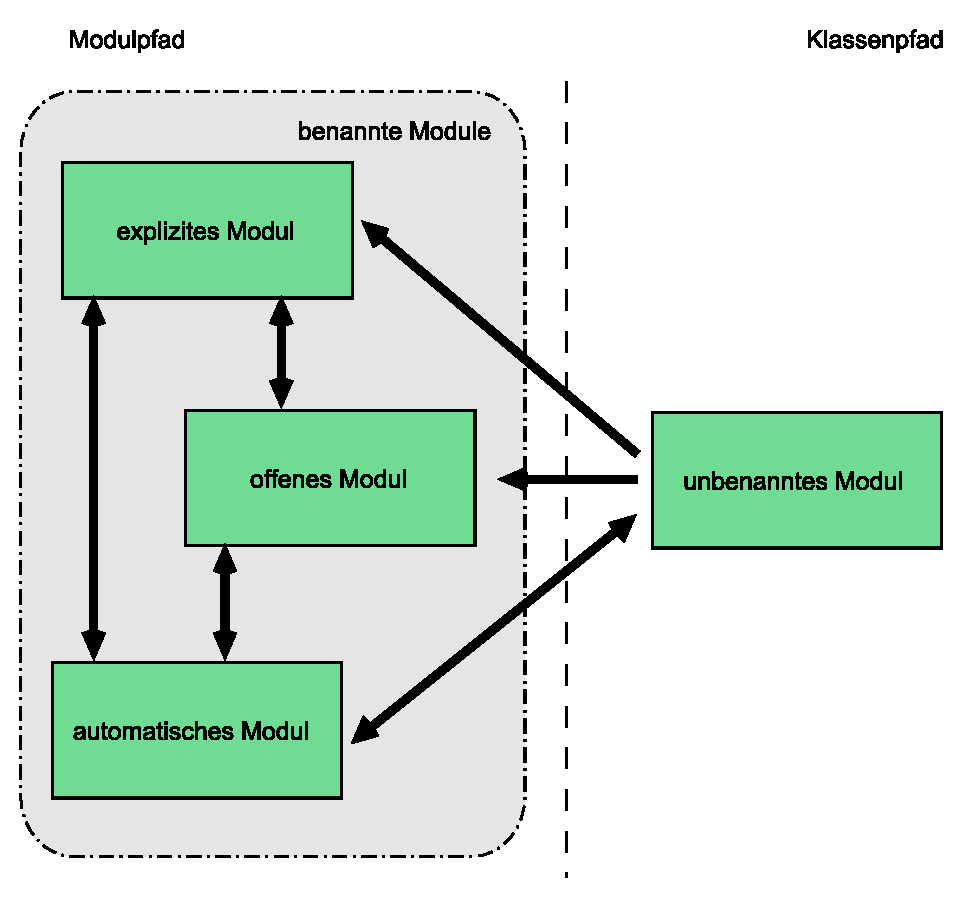
\includegraphics[width=0.7\textwidth]{material/images/module-access.pdf}
      \caption{Modulzugriffsrechte \cite{modulMitJava9}}
      \label{fig:modacc}
    \end{figure}

    Das letzte Modul beschreibt ein Modul mit speziellem Verhalten, das sich zwischen den Architekturen stellt und eine Brücke zwischen dem Modulpfad und dem Klassenpfad errichtet. Die \textit{automatischen Module} beschreiben einen Migrationsansatz der bestehenden Bibliotheken, die vom Klassenpfad auf den Modulpfad verschoben werden und keine \textit{Modulbeschreibung} besitzen. Diese kriegen einen Modulnamen zugewiesen und können über diesen von den \textit{expliziten Modulen} aufgerufen werden. Somit übernimmt Java die Kopplung der \textit{automatischen Module} mit allen \textit{expliziten Modulen}, indem alle internen Pakete für die Nutzung offengelegt werden und alle Module auf dem Modulpfad für die Verwendung importiert werden. Folglich ist eine Legacy-Bibliothek auf den Modulpfad funktionstüchtig und bietet eine ganz besondere Fähigkeit, nämlich die wechselseitige Kommunikation zwischen dem Modulpfad, sowie dem Klassenpfad. Dank dieser Fähigkeit können Bibliotheken migriert werden und beide Architekturen zugleich unterstützen. Dieses Verhalten motiviert die Entwickler ihren Code für den Modulpfad zu entwickeln, da die nötigen Legacy-Bibliotheken der Applikation zugleich in beiden Architekturen verfügbar ist.\newline
    Dennoch bringen die \textit{automatischen Module} zusätzliche Komplexität in die Architektur, indem alle explizite Module mit diesen verbunden werden. Daraus folgt eine starke Kopplung und somit eine unübersichtliche und starke Abhängigkeit zwischen den Modulen.\cite{modulMitJava9,java9modRevealed,modulProgJava9}\bigbreak

    Nichtsdestotrotz bietet das automatische, sowie das unbenannte Modul diverse Migrationsszenarien, die flexible Wege für die Modernisierung der Applikation anbieten.

  \section{Kopplung zwischen den Modulen} \label{sec:mod_kop}
    Die Einführung des Modulsystems in Java 9 integriert das Konzept der Aufteilung einer monolithischen Softwareumsetzung, in übersichtliche miteinander sachlich verbunden Modulen. Diese Idee wird zuerst von Java selbst umgesetzt, um als Beispiel für den aufbauenden Code zu fungieren. In der praktischen Umsetzung formuliert Java die Modulbeschreibung mithilfe der \textit{module-info.java} Datei, die drei Kopplungstypen enthalten kann: welche durch \textit{requires, exports} und \textit{opens} Deskriptoren beschrieben werden.

    \begin{figure}[h!]
      \centering
      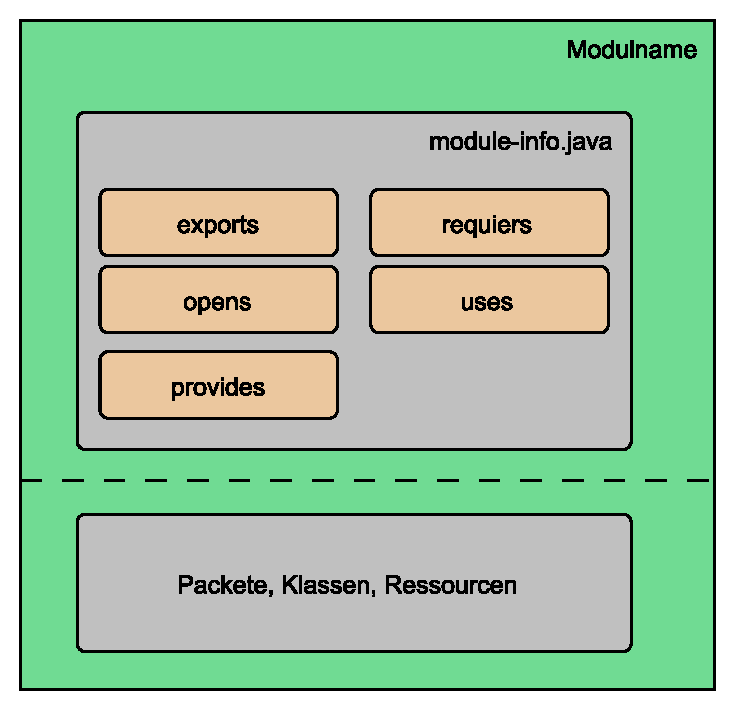
\includegraphics[width=0.5\textwidth]{material/images/module-info.pdf}
      \caption{Die Schnittstellenbeschreibung \textit{module-info.java}}
      \label{fig:module-info}
    \end{figure}

    Die in der Abbildung \ref{fig:module-info} dargestellten und vorher diskutierten Kopplungsarten, können die Zugriffsberechtigungen ferner einschränken. Diese können ihre Schnittstelle exklusiven Modulen öffnen, die fortan als eine transitive Verbindung weiter gereicht und obendrein als eine optionale Abhängigkeit deklariert werden. Die \textit{uses} und \textit{provides} Schlüssel beschreiben eine Dienstanfrage, sowie ein Dienstangebot, die durch den Java \textit{Service-Lader} miteinender verknüpft werden.\newline
    Der \textit{Service-Lader} übernimmt in diesem Fall die Rolle des Registrierungsdienstes und vermittelt das Angebot und die Nachfrage nach Funktionalität innerhalb der Applikation. Das Konzept der Dienstregistrierung und der Dienstverwaltung geht über die Grundlagen hinaus und wird hier nicht weiter diskutiert. Dessen ungeachtet, ist es eine zusätzliche Möglichkeit die Modulkopplung zu minimieren. \cite{softModDes,modulMitJava9} \bigbreak

      \begin{figure}[h!]
      \centering
      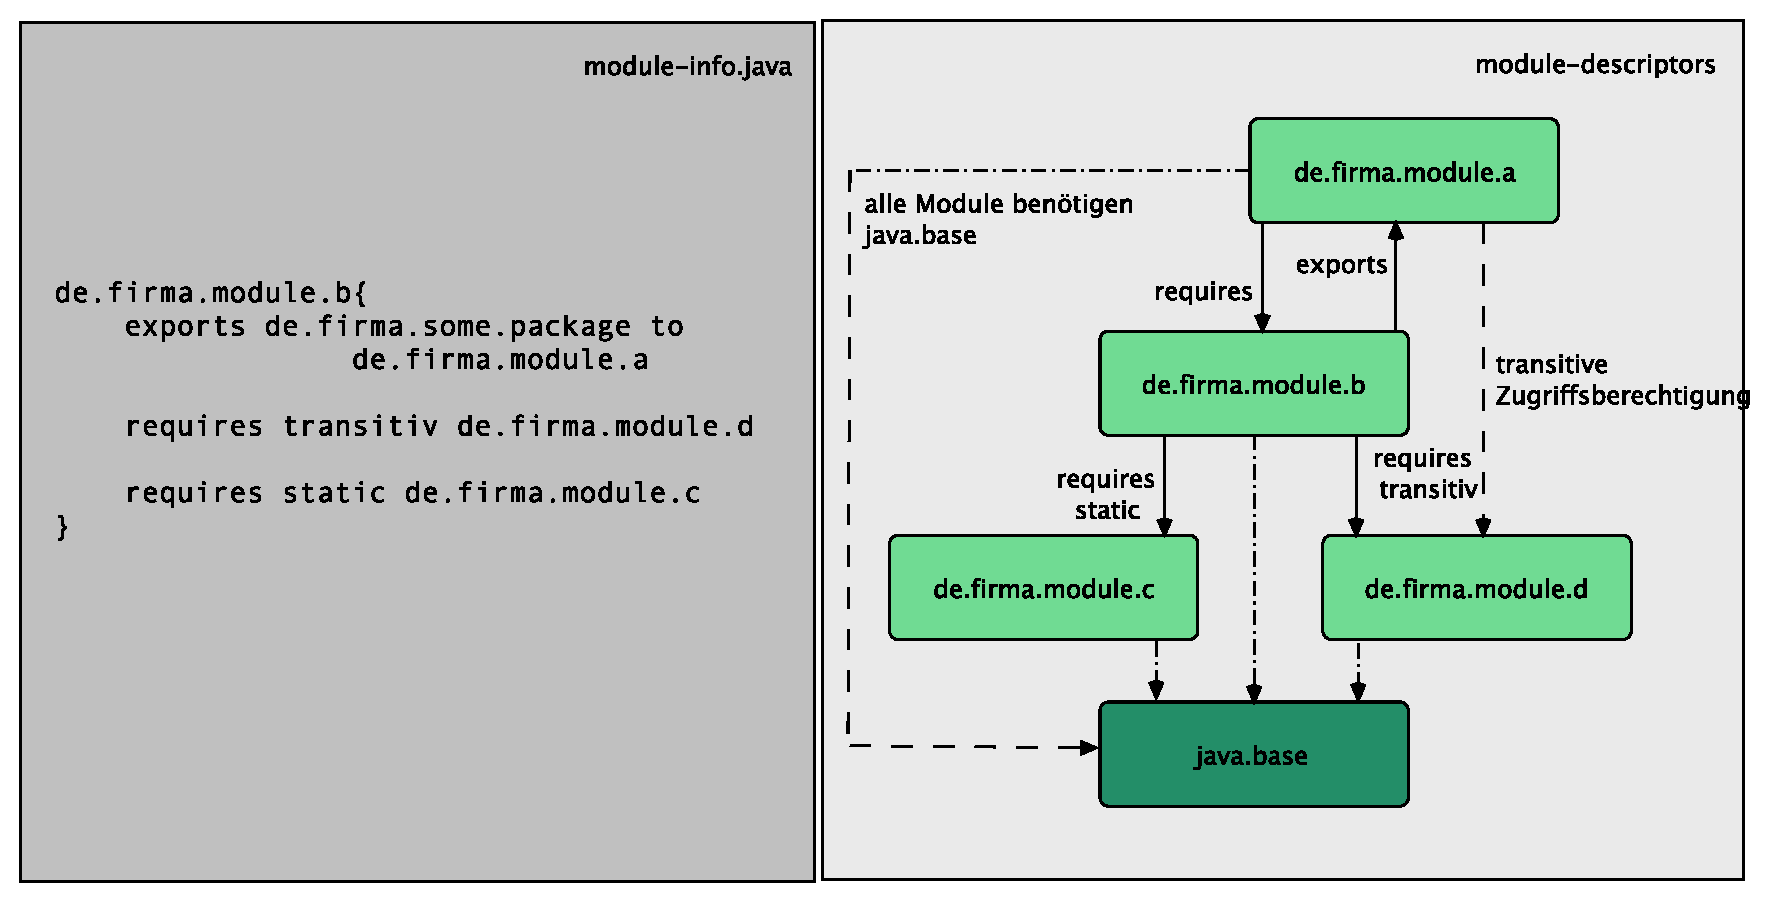
\includegraphics[width=\textwidth]{material/images/transitiv.pdf}
      \caption{Abwandlung der Kopplungsarten}
      \label{fig:abw-kopl}
  \end{figure}

    Im Folgenden werden die in der Abbildung \ref{fig:abw-kopl} dargestellten Möglichkeiten der Kopplungstypen gelistet. Zu beachten ist die Wechselbeziehung zwischen den Modulen, die Pakete anbieten und Module anfordern. \cite{jmsOracle}

    \begin{description}
      \item[requires]\hfill
      \newline \textit{requires} Modul
      \newline \textit{requires transitiv} Modul
      \newline \textit{requires static} Modul
      \newline \textit{requires transitiv static} Modul
      \item[exports]\hfill
      \newline \textit{exports} Packet
      \newline \textit{exports} Packet \textit{to} Modul-1, Modul-2
      \item[opens]\hfill
      \newline \textit{opens} Packet
      \newline \textit{opens} Packet \textit{to} Modul-1, Modul-2
      \item [uses]\hfill
      \newline \textit{uses} Dienst-Schnittstelle 
      \item[provides]\hfill
        \newline \textit{provides} Dienst-Schnittstelle \textit{with} Service-Impl-1, Service-Impl-2
  \end{description}


  Wie in der grafischen Darstellung \ref{fig:abw-kopl} abgebildet, handelt es sich bei den Kopplungstypen um Zugriffsrechte, die als ein offener Vertrag zwischen Modulen aufgestellt werden. Dementsprechend dienen die Kopplungsschlüssel nicht nur der Lesbarkeit und Autonomie, sondern erweitern die Prozedur des Klassenladens durch explizite Schnittstellen und Zugriffsberechtigungen.\cite{modulMitJava9}

  \section{Klassenladen innerhalb der Module} \label{sec:mod-cll}
    Im Abschnitt \ref{sec:nam} wurden Namensräume vorgestellt, die Klassen von einender trennen und diese als separate Software-Komponenten behandeln, um die Sichtbarkeit der Codebasis gegenüber dem Restsystem abzugrenzen. Jedoch bring dieses Feature einen großen Aufwand mit sich. Denn sofern die Applikation eine große Anzahl an Bibliotheken benutzt und jedes davon auf einem eigenen Klassenlader betrieben werden soll, wächst der Wartungsaufwand mit der Anzahl der Bibliotheken.\newline
    Mithilfe der Module und deren neuem Ansatz der internen Kapselung, soll dieses Problem adressiert werden, indem separate Zugriffsräume für jedes Modul innerhalb eines Klassenladers definiert werden. Diesen stellen sicher, dass dass die interne Struktur eines Moduls während der Laufzeit nicht kompromittiert werden kann.\newline
    Für die Garantie der Modulkapselung, wird das im Abschnitt \ref{sec:cls} vorgestellte \textit{Java Klassenlader-System} nicht ersetzt, sondern mit zusätzlichen Kontrollen versehen, die strikt nach deklarierten Modulbeschreibung Zugriff gewährleisteten. Im Falle der Nichteinhaltung der Zugriffsrechte zwischen den Modulen, wirft der Klassenlader neue Fehlermeldungen, wie die \textit{IllegalAccessException} oder die \textit{IllegalAccessError}. Somit bleibt die ehemalige Klassenlader-Hierarchie erhalten, die an das Modulsystem von Java angepasst worden ist. \cite{classLoadingOracle, modulMitJava9}\bigbreak

    Um die neuen Kontrollmechanismen im Java Kern zu verankern, wurde die \textit{rt.jar}, die für die Ausführung von Java Code zuständig ist, auf Module mit expliziten Aufgabenbereichen aufgeteilt. Wie in der Abbildung \ref{fig:jdk} abgebildet, beschäftigt sich das aktualisierte \textit{Klassenlader-System} mit dem Laden bestimmter Module, die in Gültigkeitsbereiche fragmentiert sind. Diese nutzen immer noch das Delegierungsmodell \ref{sec:dm} und delegieren jede Anfrage zuerst an den Wurzel-Klassenlader. Mit dem Modulsystem von Java wurde dieses Verfahren durch zwei Sicherheitsverfahren erweitert. Das erste Verfahren löst eins der größten Schwierigkeiten der Java Entwickelung, nämlich das Management der Abhängigkeiten eines Systems. Diese Herausforderung wird als \textit{Jar-Hell} bezeichnet und beschreibt eine komplexe Applikation, die eine lange Liste an genutzten Drittanbieter-Bibliotheken benötigt. Hier taucht das Problem auf, dass der Applikations-Code den Klassenpfad nicht kontrolliert und annehmen muss, dass alle benötigten Bibliotheken auf den Klassenpfad vorhanden sind. Die lokal eingerichtete Maschine oder Entwicklungsumgebung kann das Management verwalten, jedoch kann diese nicht garantieren, dass die Software in einer anderen Umgebung funktionsfähig bleibt.\newline
    Dieser Anforderung hat sich das Modulsystem von Java gestellt und bietet die phasenübergreifende Wiedergabetreue auf allen Systemen, indem jedes Modul eine Voraussetzung deklariert, die der Modulpfad erfüllen muss, bevor die Applikation ihre Arbeit beginnt. Somit wird das gleiche Verhalten, sowie Fehlerprüfungen in der Kompilierungs- und Ausführungsphase erreicht.\newline
    Das zweite Verfahren garantiert die Einhaltung der Nutzungsrechte einer Bibliothek, indem die Nutzung einer Bibliothek über klar definierte Schnittstellen geschieht und unterbindet somit den impliziten Zugriff auf den Inhalt innerhalb eines Namensraums. Beide Verfahren berufen sich auf die \textit{module-info.java} Konfigurationsdatei, in der die benötigte Information verankert ist. \bigbreak

    Um die Klassen aus dem Modulpfad zu laden, wurde das \textit{Klassenlader-System} an den Modulpfad angepasst und lädt jetzt Module, die nach Sicherheitsberechtigungen bestimmten Klassenlader zugewiesen werden. Der \textit{Bootstrap}-Klassenlader ist der Klassenlader der JVM und genießt alle Sicherheitsprivilegien. Dieser lädt die \textit{Core Java-SE} und \textit{JDK-Module}, wie \textit{java.base} und \textit{java.logging}. Der Extension-Klassenlader wurde von dem Plattform-Klassenlader ersetzt und lädt jetzt die \textit{Plattform Java-SE} Module, wie zum Beispiel die \textit{java.sql}, oder die \textit{java.xml.ws} Bibliotheken. Und zuletzt bleibt der Applikation-Klassenlader, der die Applikationsmodule auf dem Modulpfad verwaltet. \cite{classLoadingOracle,modulMitJava9,java9modRevealed}

  \section{Das Modulschichten Konzept} \label{sec:module_layers}
     Obwohl das Klassenlader-Konzept von Java seine Gültigkeit behält, gibt es mit dem Einzug der modularisierten Plattform einige Änderungen.\newline 
     Mit dem Modulsystem von Java wird ein neues Konzept der Modulschichten eingeführt, das für das Laden von Java Code während der Laufzeit verantwortlich ist. Die Modulschichten kapseln, validieren und laden bestimmte Modulgruppen, die während der Laufzeit in die Applikation integriert werden können. Dazu zählen explizite, offene, sowie unbenannte Module. \newline
     Das Laden von zusätzlichem Code war bereits mit dem Klassenlader-System möglich, indem zusätzliche Klassenlader instanziiert und ausgetauscht werden konnten, jedoch besitzen die Klassenlader keine Mechanismen zum Validieren des eingelesenen Codes, sodass unerwartetes Verhalten im Betrieb der Applikation zu jedem Zeitpunkt auftreten kann. \newline
     Mithilfe der Modulschichten wird das bestehende Klassenlader-Konzept erweitert, indem zusätzliche API's für die Verwaltung von dem dynamischen Code eingeführt und das zusätzliche Erzwingen der Korrektheit der Modulabhängigkeiten innerhalb des Systems, garantiert wird.\bigbreak

    \begin{figure}[h!]
      \centering
      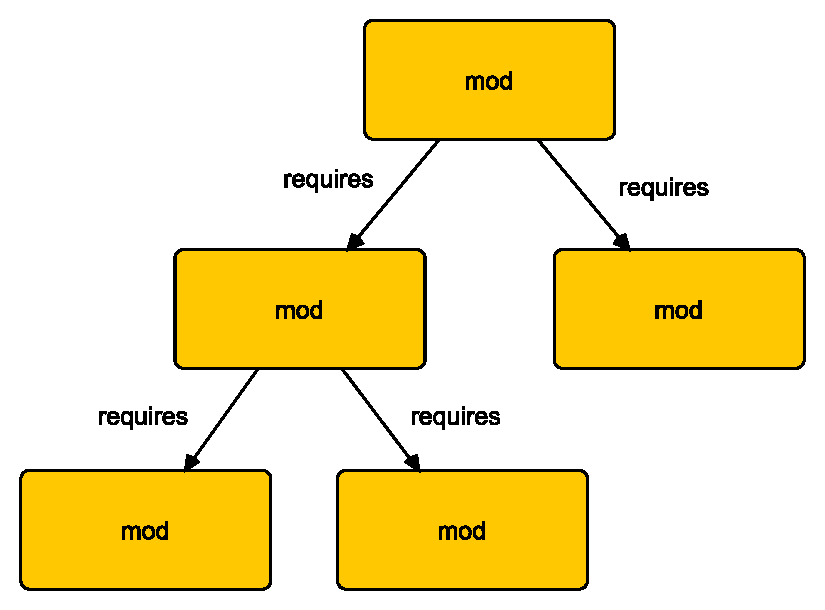
\includegraphics[width=0.8\textwidth]{material/images/module-graph.pdf}
      \caption{Modulgraph \cite{javaMod9}}
      \label{fig:module-graph}
    \end{figure}

     Das Laden von zusätzlichen Modulen geschieht in zwei Phasen: Zuerst wird eine Konfiguration erstellt, die ausgewählte Module für das Laden in die Applikation aufnimmt. Die Konfiguration benötigt eine Modulmenge, sowie die ausgewählte Wurzel-Module, aus den anschließend alle Modulabhängigkeiten ermittelt und validiert werden. Dafür wird ein neu eingeführtes Objekt genutzt, nämlich der \textit{Modul-Sucher}, der für ein gegebenes Verzeichnis die Metainformationen aller Module ausliest und für die Nutzung bereitstellt. \newline
     Im nächsten Schritt müssen die gefundenen Module auf Konsistenten geprüft werden. Dazu wird ein Modul Graph \ref{fig:module-graph} erzeugt, der aus den gegebenen Wurzel-Modulen alle geforderten Modulbeziehungen auflöst. Er inspiziert \textit{Split Packages}, \textit{Zyklen}, valide Zugriffsrechte und erklärt im Anschluss den Code für ausführbar. Dieser stellt sicher, dass alle Abhängigkeiten, einschließlich der indirekten Abhängigkeiten, aufgelöst werden können.\newline
     Das Ergebnis besteht aus einer betriebsfähigen Konfiguration mit einer Strukturgrafik der aufgelösten Abhängigkeiten, die für die Ausführung im Applikationskontext benötigt wird. \cite{java9modRevealed}\bigbreak 

    \begin{figure}[h!]
      \centering
      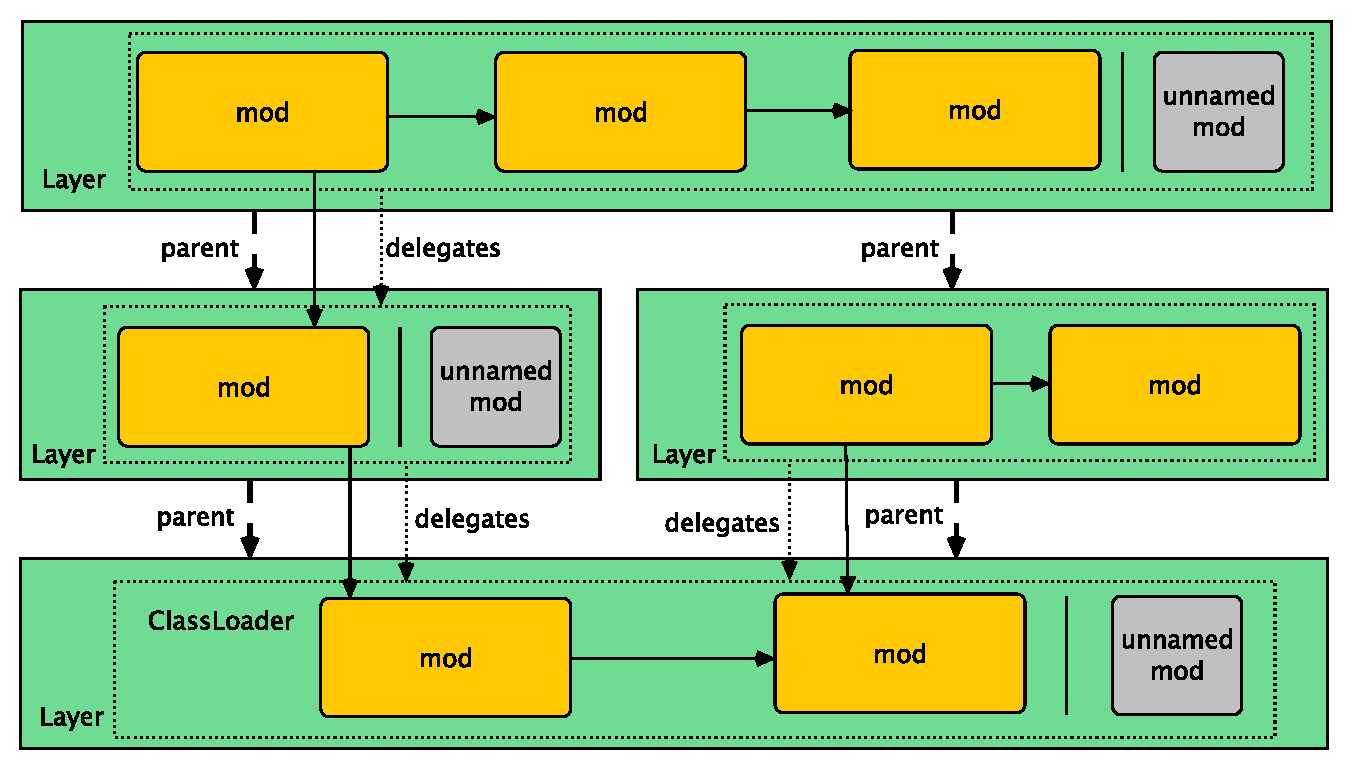
\includegraphics[width=\textwidth]{material/images/module-layer.pdf}
      \caption{Modulschicht \cite{javaMod9}}
      \label{fig:module-layer}
    \end{figure}

    Nachdem die Konfiguration ausgewertet wurde, kann eine Modulschicht erstellt werden, die alle Module der konsistenten Konfiguration instanziiert. Dafür wird ein neuer Klassenlader von der Modulschicht erstellt und eine Hierarchie aufgebaut, die auf meherere übergeordnete Modulschichten, sowie einen Klassenlader verweist. Dementsprechend referenziert der Modulschicht-Klassenlader immer auf einen übergeordneten Klassenlader, um dem ehemaligen Delegierungsmodell zu entsprechen und die Funktionalität der \textit{unbenannten Module} weiterhin erfüllen zu können. Des Weiteren, referenziert die Modulschicht selbst auf eine variable Menge von übergeordneten Modulschichten, die das Auflösen der benötigten benannten Modulabhängigkeiten unterstützen und die Modulsuche an entsprechenden Modulschichten weiterleitet. \bigbreak

    Das neue Konzept der Modulschichten erweitert das bestehende System der selbst erstellten hierarchischen Namensräume, indem Modulabhängigkeiten beim Laden in die Applikation validiert, gruppiert und aktiv verwaltet werden können. Darüber hinaus enthält die Modulschicht-Konfiguration die komplette Information über den Inhalt ihrer Schicht, sowie der darunterliegenden Modulschichten. \newline
    Die Konfiguration von dem dynamisch nachgeladenen Code, der Schichtübergreifend validiert wird, verhindert das Überlagern des bereits integrierten Codes und ändert die Art und Weise, wie die Suche nach Modulklassen durchgeführt wird. \newline
    Die Klassensuche wird nun mit der \textit{direkten Delegation} durchgeführt, die zuerst die eigene Schicht bevorzugt, bevor die Anfrage an die darüberliegende Schicht weiterleitet wird. Die übergeordnete Schicht verhält sich nach demselben Prinzip und versucht zuerst selbst die Klasse zu laden, bevor die nächste Delegation durchgeführt wird. \bigbreak

    Kurzgefasst, gehören Schichten zu Modulen wie Klassenlader zu Klassen; also ein Mechanismus zum Laden und Instanziieren von Elementen mit erweiterten Diensten und Sicherheitsbestimmungen.\cite{javaMod9,parentDelegationModel,modulMitJava9}

  \section{Der Service-Lader} \label{sec:servLoad} 
    Die Java Version 1.6 führt ein Konzept der Dienste ein, die eine bessere Entkopplung zwischen Klassen unterstützt, indem Klassenabhängigkeiten erst zur Laufzeit aufgelöst werden können. Dadurch wird eine Entkopplung zwischen den Anbieter-Klassen und den später auf diese zugreifenden Nutzer-Klassen erreicht, indem die Klassenbindung nicht über eine direkte Implementierung, sondern über eine Schnittstelle umgesetzt wird. Über den \textit{Service-Lader} kann anschließend auf die einzelne Implementierung-Instanz zugegriffen werden. \bigbreak
    \begin{figure}[h!]
      \centering
      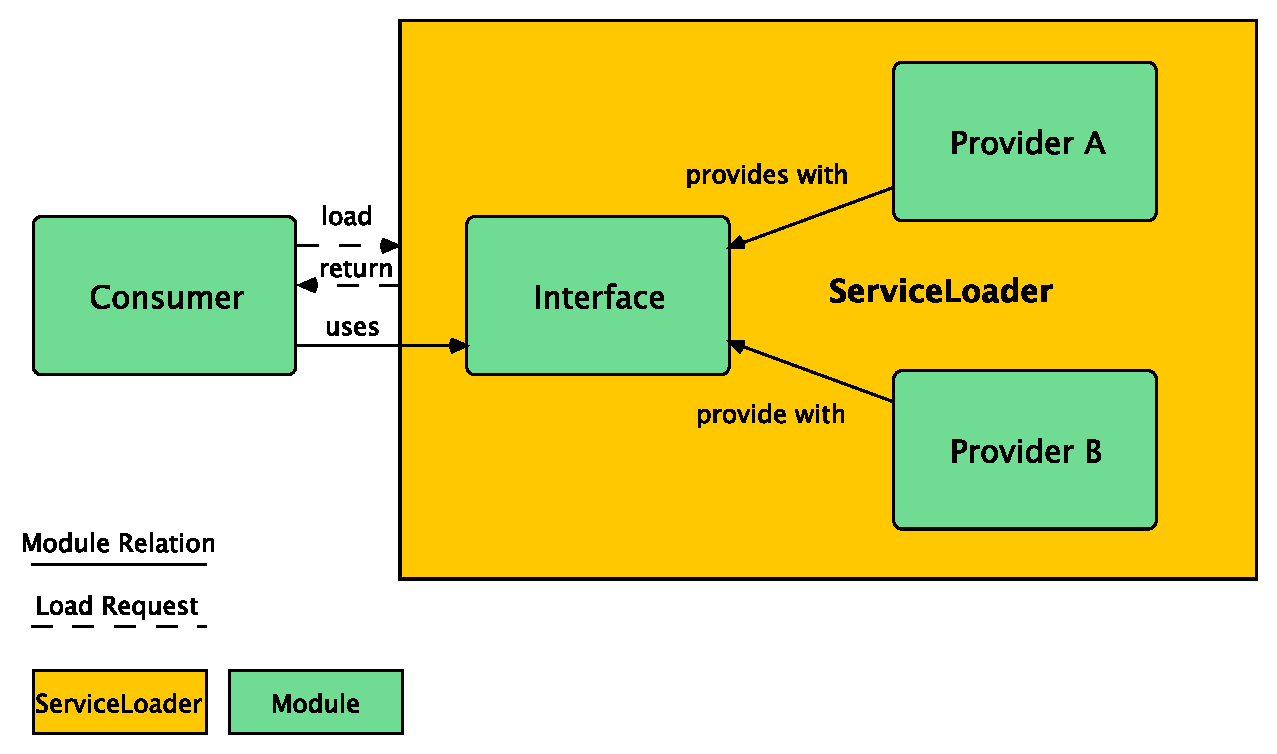
\includegraphics[width=0.8\textwidth]{material/images/ServiceLoadingMulti.pdf}
      \caption{Service-Lader Konzept}
      \label{fig:serviceLoaderMulti}
    \end{figure}
    Die Dienst–Anbieter und Dienst-Nutzer lassen sich in der \textit{module-info.java} Konfigurationsdatei definieren und zur Laufzeit lässt sich die Implementierung eines bestimmten Dienstes von der Applikation wählen, ohne dass zuvor eine explizite Abhängigkeit zwischen diesen Modulen deklariert wurde. \bigbreak

    Der Java \textit{Service-Lader} spielt eine wichtige Rolle für die Entkopplung der Module. Dieser sucht  Applikation nach angebotenen Diensten für eine entsprechende Schnittstelle ab, und versorgt den Nutzer mit einer möglichen Umsetzung. Somit können mehrere gleiche oder unterschiedliche Dienste in der Applikation existieren und vom Nutzer entkoppelt, abgefragt und ausgeführt werden. Dafür wird in der \textit{module-info.java} mit den \textit{provides with} und \textit{uses} Schlüssel die Dienstkommunikation etabliert und über den \textit{Service-Lader} umgesetzt. Somit dient die \textit{Service-Lader} Instanz innerhalb der Applikation als ein Registrierungsdienst.\bigbreak


    In der Abbildung \ref{fig:serviceLoaderMulti} ist ein Nutzermodul abgebildet, welches ein Dienst des Schnittstellen-Moduls anfordert. Die Suche nach einem Dienst für die angefragte Schnittstelle, übernimmt der \textit{Service-Lader} und instaziiert eine Liste an möglichen Anbietern. Der Nutzer kann anschließend entscheiden, welche Implementation er nutzen möchte.   


\section{Der modularisierte JDK} \label{sec:modular_java_base}
  Um die aufgestellten Regeln und Konzepte des entworfenen Modulsystems in Java zu integrieren, muss die Java Plattform diese selbst als Vorreiter erfüllen. \bigbreak
  Demnach wurde die Laufzeitumgebung (\textit{Run-Time}), die aus der \textit{rt.jar} besteht, auf Module aufgeteilt und miteinander über Kommunikationsregeln und Schnittstellen verknüpft. Das Ergebnis der modularisierten \textit{rt.jar} ergab 70 Module, die sich gegenseitig ergänzen. \newline
  In der Konsequenz ist eine kleine Applikation, die sich nur an dem \textit{base} Modul bedient, mit einem Speicherbedarf von 16 MB umsetzbar. Im Gegensatz dazu, müssten für ein paar Zeilen Code in der 8 Version von Java, 160 MB der \textit{rt.jar} in die Laufzeitumgebung miteinbezogen werden, um den Laufzeitanforderungen zu entsprechen.\bigbreak
  \begin{figure}[h!]
   \centering
   \includegraphics[width=\textwidth]{material/images/moduleGraph.jpg}
   \caption{Modularisierte \textit{rt.jar} Laufzeitumgebung \cite{modGraph}}
   \label{fig:jdk}
  \end{figure}
  Obwohl das Modulsystem viele Neuerungen und Aufwertungen der Java Plattform mit sich brachte, konnten nicht alle Wünsche erfüllt werden. Wie zum Beispiel das Nutzen gleichnamiger Bibliotheken mit unterschiedlicher Versionsnummer.\newline
  Dennoch gibt es Ansätze, die es erlauben, eine Versionsnummer in einem Modul zu verankern und somit existiert die Wahrscheinlichkeit, dass diese Fähigkeit in der Zukunft nachgerüstet wird. 
 


\chapter{Migration}

	In dem vorherigen Kapitel wurden Module und ihre Eigenschaften, Konstruktionsregeln sowie Modularten behandelt. Dieses Kapitel beschäftigt sich mit der Fragestellung, wie Altsysteme, die vor dem Modulsystem von Java entwickelt wurden, in dem Modulkontext betrieben werden können und was getan werden muss, um diese den modernen Anforderungen anzupassen und zu modularisieren.\bigbreak

	Die Migration behandelt Systeme, die nicht beständig auf dem aktuellen Stand der Technik gehalten werden können und an ihren Ausführungskontext gebunden sind. Diese rutschten langsam in den Bereich der Altsysteme, bis ihr Lebenszyklus zu Ende geht und der Legacy-Zustand erreicht ist. Um die Systeme weiterhin zu nutzen, müssen sie in eine Umgebung mit den geforderten Eigenschaften, ohne Änderungen der internen Struktur vorzunehmen, übertragen werden. Dieses Verfahren wird oft im Bereich der Softwaretechnik mit Software Reengineering und Software Neuimplementation verwechselt, dessen Ziel in der Optimierung der Codebasis liegt und nichts mit dem Ausführungskontext zu tun hat. \cite{martens2016ablosung} \bigbreak

	% Migrationsmethoden und der von ihnen gelösten Problemen. 
	Während des Betriebs einer lang gepflegten Kernapplikation, wird der Lebenszyklus öfter überschritten und muss den Migrationszyklus mehrmals durchlaufen. Zum Beispiele kann eine Applikation an Größe gewinnen und muss in die Cloud ausgelagert werden, die Anforderungen können sich verschieben und der Technologie-Stack muss an die Marktbedürfnisse angepasst werden, darüber hinaus kann der Ausführungskontext einen großen Versionssprung hinter sich lassen, der das Warten der Software unter den momentanen Bedingungen unmöglich macht. \newline
	Dem zufolge ist das Umfeld der Software Entwicklung eine dynamische Umgebung, denn auch mit einer gut durchdachten Architektur kann nicht garantiert werden, dass in der Zukunft heutige Paradigmen, Werkzeuge und Aufgabenbereiche denselben Kurs behalten. Deswegen existieren bereits sämtliche Migrationsstrategien, die als ein Leitfaden den Entwickler durch die Migration führen. \bigbreak

	Im folgenden Kapitel werden Ansätze vorgestellt, die Monolithische- sowie Bibliotheksanwendungen in das modulare System überführen ohne Änderung an der internen Funktionalität durchzuführen. 


\section{Legacy-System}

	Der Begriff \textit{Legacy-System} beschreibt ein altes System, das innerhalb einer Organisation länger als der geplante Lebenszyklus in Betrieb bleibt. Der englische Begriff \textit{Legacy}, zu Deutsch Erbe, bezieht sich nicht auf das Alter der Software, sondern auf die Interpretation der Software als Erbe. Da die Umsetzung von früheren Entwickler Teams durchgeführt wurde, die sich an damaligen Konzepten und Strategien bedienten, ergab die Lösung ein Erbe mit bestimmten Einschränkungen, die für die zukünftige Erweiterung der Software eine große Rolle spielen. Denn die typischerweise veralteten Verfahren und Technologie lange Lebenszyklen mit umfangreichen Veränderungen und Erweiterungen erfahren haben \cite{sneed2016softwaremigration}. \bigbreak

	Zu meist handelt es sich um sogenannte Kernsysteme zur Unterstützung wesentlicher Geschäftsprozesse eines Unternehmens. Sie sind in der Regel geschäftskritisch und können nicht ohne großen Aufwand und Risiko für das Unternehmen ausgetauscht werden. Aufgrund ihres langen Lebenszyklus, ihrer Komplexität und ständigen Überarbeitungen, ist die Logik solcher Systeme oft unübersichtlich und schlecht dokumentiert. Ihre Implementierung kann zusätzlich früher geltenden Standards unterliegen und anderen Programmierparadigmen folgen, die nur schwer verständlich sind. Daher sind Geschäftsprozesse und Geschäftsregeln im Code versteckt und müssten z.\,B. für eine Neuimplementation erst rekonstruiert werden \cite{martens2016ablosung}.

\section{Migration} \label{ssub:migration}

	% schau in diesem buch nach einer defenition  mit den storchen 
	Die Softwaremigration bezeichnet die Überführung eines Softwaresystems in eine andere Zielumgebung oder in eine sonstige andere Form, wobei die fachliche Funktionalität unverändert bleibt. Als Ausgangspunkt steht dabei immer ein bestehendes System, das an Anforderungen und Techniken des Anwendungsbereiches angepasst werden muss \cite{sneed2016softwaremigration}. Die Adaption an den neuen Anwendungsbereich geschieht zu meist nicht problemlos und muss system- und kontextbezogene Hürden überwinden. 

\section{Migrationshürden} \label{MigH}

	% Einleitung: hier kommen allgemeinen Beispiele der Migrationsproblematik 
	Die Migrationshürden sind fest mit dem Anwendungskontext verbunden und hängen stark von der Beschaffenheit der neuen Umgebung ab. Da in unserem Fall die Migration innerhalb der Java Umgebung stattfindend, müssen die Neuerungen des Modulsystems analysiert und auf den bestehenden Zustand der Applikation abgebildet werden.\bigbreak

\begin{itemize}
	% Hauptteil: Probleme und Hürden, die der neue Kontext macht
	\item Die Probleme des Modulsystems beginnen mit den Zugriffsrechten auf die Core-JDK API's. Diese sind ab sofort in dem Modul gekapselt und bieten nur eingeschränkte Möglichkeiten Aufrufmöglichkeiten. Nichtsdestotrotz stellt Java für viele der gekapselten API's einen Ersatz zur Verfügung, wodurch zahlreiche Probleme mit einem relativ geringen Aufwand behoben werden können. \cite{masteringJava9,modulProgJava9,modulMitJava9,javaMod9} 


	\item Im Weiteren verbietet das neue Modulsystem namensgleiche Pakete in verschiedenen Modulen. Dieses adressiert das vorher besprochene Problem aus dem Kapitel \ref{sec:nam}, nämlich den Zugriff auf privat deklarierte Pakete aus fremden Modulen. Trotzdem gibt es Bibliotheken mit ähnlicher Paketstruktur, die sich nicht böswillig sich Zugriff verschaffen wollen, sondern spiegeln eine Standardstruktur einer Bibliothek widerspiegeln, wie zum Beispiel \textit{de.firma.input.reader} kann in mehreren Bibliotheken eines Unternehmens existieren kann und ab Java 9 nicht mehr zulässig sein wird. Somit müssen Module mit ähnlicher Struktur angepasst werden, um den nächsten Modularisierungsschritt durchführen zu können. \cite{masteringJava9,modulProgJava9,modulMitJava9,javaMod9} 


	\item Der Klassenlader-Typ des Applikation-Klassenladers wurde überarbeitet und infolgedessen auch das Arbeiten mit den ehemaligen URL-Klassenlader Methoden. Der bestehende Code, der den URL- Klassenlader exzessiv nutzt und zum Beispiel Ressourcen aus verschiedenen Quellen lädt, muss auf den \textit{Secure-Klassenlader} oder  \textit{Klassenlader} aufgewertet werden, um funktionstüchtig zu bleiben. \cite{oracModClassLoader,jecan2017java} 


	\item Einer der kritischen Veränderungen, die die Modultatform mit sich bringt, ist das Verbot von zyklischen Abhängigkeiten von Modulen untereinander. Diese dürfen sich nicht gegenseitig mit dem Schlüssel \textit{require} koppeln, da sonst eine Veränderung in einem Modul zwangsläufig eine Änderung in den anderen Modulen hervorrufen kann. Dieser Stil kann sich schnell über die ganze Applikation verbreiten und kleine Änderungen an einer Stelle zu unübersichtlichen Seiteneffekten führen. Genau diese Probleme adressiert das Modulsystem in erster Linie und verbietet aus diesem Grund Zyklen in dem Applikationsentwurf. Um bestehende Zyklen in einer Applikation zu lösen, muss die Funktionalität genau betrachtet und in kleine unabhängige Aufgaben aufgeteilt werden. Somit werden Zyklen aufgebrochen und die Aufgabenstellung jedes Moduls klar definiert. \cite{java9modRevealed,modulProgJava9,modulMitJava9} 
\end{itemize}

\section{Migrationsarten} \label{Migratiosarten}

	% Schluss: Bewegen uns auf die möglichen Migrationsstrategien für die Modularisierung.
	Da jede Applikation spezifisch Migrationsanforderungen besitzt, gibt es unterschiedliche Verfahren, die sich bestimmten Kriterien widmen. Dementsprechend sollte man die gegebene Applikationsbeschaffenheit ermitteln und dessen Probleme auf die passende Migrationsstrategie abbilden. Die prominenten Migrationsstrategien der Software Techniken sind \textit{Chicken Little} und \textit{Butterfly}, zwei der gängigsten Arten der Softwaresystem Migration. \cite{sneed2016softwaremigration} \bigbreak


	% Chicken Little
	Softwaresysteme, die nach dem \textit{Chicken-Little-Ansatz} migriert werden, zerlegen das System in mehrere Migrationspakete, die einzeln in kleinen inkrementellen Schritten in die neue Zielumgebung überführt werden. Damit der Betrieb des Systems nicht für die Zeitdauer der Migration ausfällt, existieren alte, neue und migrierte Teilsysteme nebeneinander. Die korrekte Kommunikation der Softwarebausteine muss über entsprechende Kommunikationskanäle errichtet werden und gestaltetet damit eine Brücke zwischen Alt- und Neuentwicklung, die zusammen eine gemeinsame Ressourcenbasis nutzen können. \cite{sneed2016softwaremigration} \bigbreak

	% Butterfly 
	Der \textit{Butterfly-Ansatz} geht von einer separaten Entwicklung der Applikation in der neuen Umgebung aus. Dies hat zur Folge, dass die Altapplikation in Betrieb bleibt und unverändert ihre Aufgabe erfüllt, bis der Nachfolger, der parallel zu dem Betrieb entwickelt und getestet wird, die Funktion korrekt widerspiegeln kann. Im Anschluss werden Ressourcenbestände in kleinen Paketen an die Applikation im neuen Kontext transferiert und das Altsystem abgeschaltet. Das Butterfly-Verfahren vermeidet also während der Migration den simultanen Zugriff auf Legacy- und Zielsystem. \cite{sneed2016softwaremigration} \bigbreak

	% Ein text der auf die nächsten Kalitel einführt 
	Zwischen den beiden vorgestellten \textit{Migrationsideen} hat sich das Java Team für die Unterstützung der Schrittweise-Migration entscheiden, die eine Applikation in kleine Softwareeinheiten aufteilt und langsam auf den neuen Modulpfad migriert. Der parallele Betrieb der neuen sowie alten Struktur wird durch eine interne Brücke, die korrekte Kommunikation zwischen den Klassenpfad und den Modulpfad errichtet umgesetzt. Die Implementation der Kommunikationsbrücke und ihrer Charakteristika, die eine kritische und verantwortungsvolle Aufgabe in dem Migrationsprozess trägt, wird für uns von dem Java Team zur Verfügung gestellt. Somit unterstützt und führt das Modulsystem von Java den Entwickler bei der Hand zu der korrekten, sicheren, modernen und funktionstüchtigen Modularchitektur. \newline
	Ungeachtet dessen, ist die Migration einer Applikation zu diesem Zeitpunkt nicht zwingend und kann innerhalb des Modulsystems weiterhin betrieben werden, da diese keine speziellen Hilfsmittel von der Umgebung fordern.\bigbreak

	In den nachfolgenden Kapiteln werden unterschiedliche Varianten der Migration und des Betriebs einer Applikation innerhalb des Modulsystems vorgestellt. 


\subsection{Plattform Migration}
	Die simpelste Migration ist eine reine Plattform Migration, ohne Änderungen an der Software vorzunehmen, wie in der Abbildung \ref{fig:PM} dargestellt. Dies ist möglich, dank der Unterstützung des Klassenpfades, der in diesem Fall die Applikation als ein \textit{unbenanntes Modul} im Modulsystem betreibt. Wie bereits im Kapitel \ref{Modularten} angesprochen, bietet dieses Modul den Betrieb der Legacy Anwendung in der neuen Umgebung mit dem geringen Anteil der möglichen Vorteile, wie zum Beispiel den Sicherheitsupdates. Zusätzlich behält die Applikation ihre monolithische Architektur und vermisst alle Modulsystem Features, die im Kapitel \ref{sec:ZdM} und \ref{sec:ME} angesprochen wurden.

	\begin{figure}[h]
		\centering
	    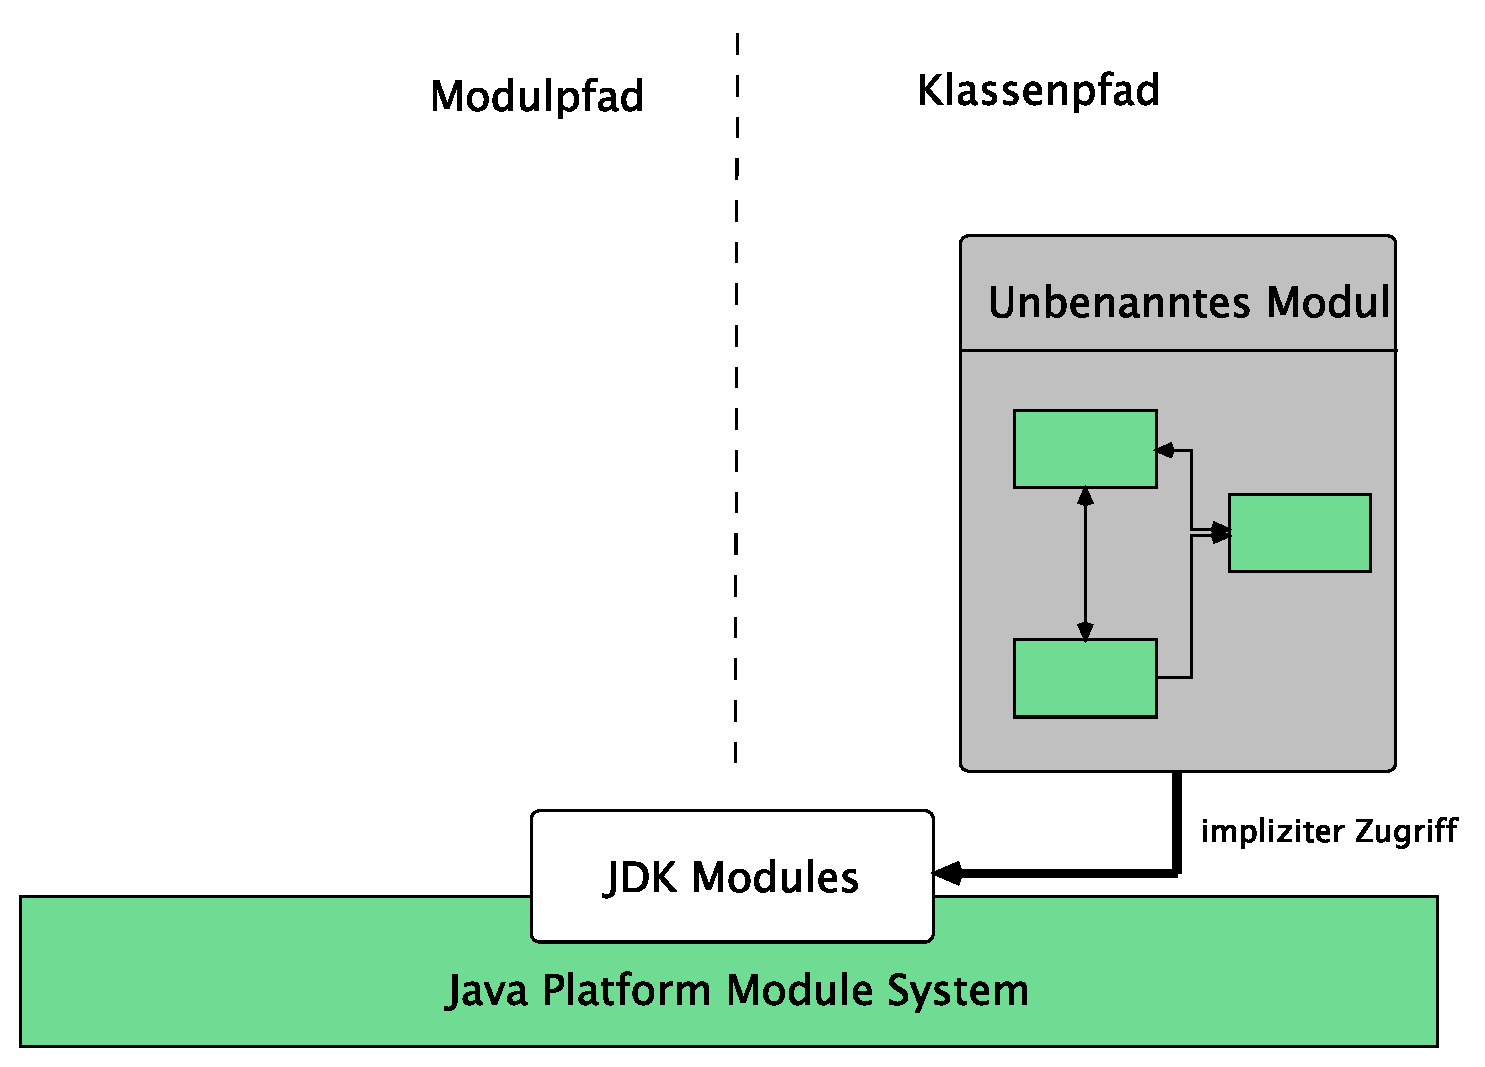
\includegraphics[width=0.8\textwidth]{material/images/platform-migrate.pdf}
	    \caption{Plattform Migration \cite{modulMitJava9}}
	    \label{fig:PM}
  	\end{figure}

	Eine weitere Möglichkeit wäre es, die Applikation und ihre Bibliotheken auf den Modulpfad zu migrieren und als \textit{automatische Module} zu betreiben. Somit wäre der alte Klassenpfad  nicht mehr im Applikationsdesign vorgesehen und fokussiert die Entwickler auf die Arbeit mit dem Modulpfad. Dennoch lässt sich nicht jede Anwendung in diesem Still migrieren, denn die Hürden aus dem Kapitel \ref{MigH}, wie die \textit{Zyklenfreiheit} sowie das Verbot der \textit{Split-Packages} in Legacy-Bibliotheken nicht immer gegeben ist. 



\subsection{Top Down Migration}
	Die \textit{Top-Down} Migration behandelt die Migration von oben nach unten, dabei werden zuerst die Applikation und im Nachhinein die Drittanbieter-Bibliotheken migriert. Dafür müssen die Applikationspakete auf Abhängigkeiten geprüft und entsprechende Module sowie Modulbeschreibungen nach den im Kapitel \ref{sec:MEK} besprochenen Kriterien erstellt werden. Mit dieser Methode werden die Drittanbieter Bibliotheken zuletzt betrachtet, da es sich bei diesen um Fremdcode handelt. \newline
	Da nach der Prüfung der Abhängigkeiten ein Graph entsteht, verweist dieser ab einem gewissen Punkt auf die Bibliotheksabhängigkeit der Applikation, die wiederum von weiteren Bibliotheken abhängen. Somit kann die Wurzel der benötigten Drittanbieter-Bibliotheken einer Applikation ausfindig gemacht und als \textit{automatische Module} in den Modulpfad eingebunden werden. Somit können diese, wie bereits in im Kapitel \ref{Modularten} behandelt, sowohl mit der Applikation als auch mit den Legacy Elementen ihrer eigenen Abhängigkeiten zugleich interagieren. Zum Schluss kümmert man sich um die Bibliotheken auf dem Klassenpfad, indem diese ersetzt oder selbständig weiterentwickelt werden, mit dem Ziel die Gesamtapplikation auf dem Modulpfad zu übertragen. \cite{javaMod9,modulProgJava9,java9modRevealed,modulMitJava9,masteringJava9}\bigbreak
	\begin{figure}[h]
		\centering
	    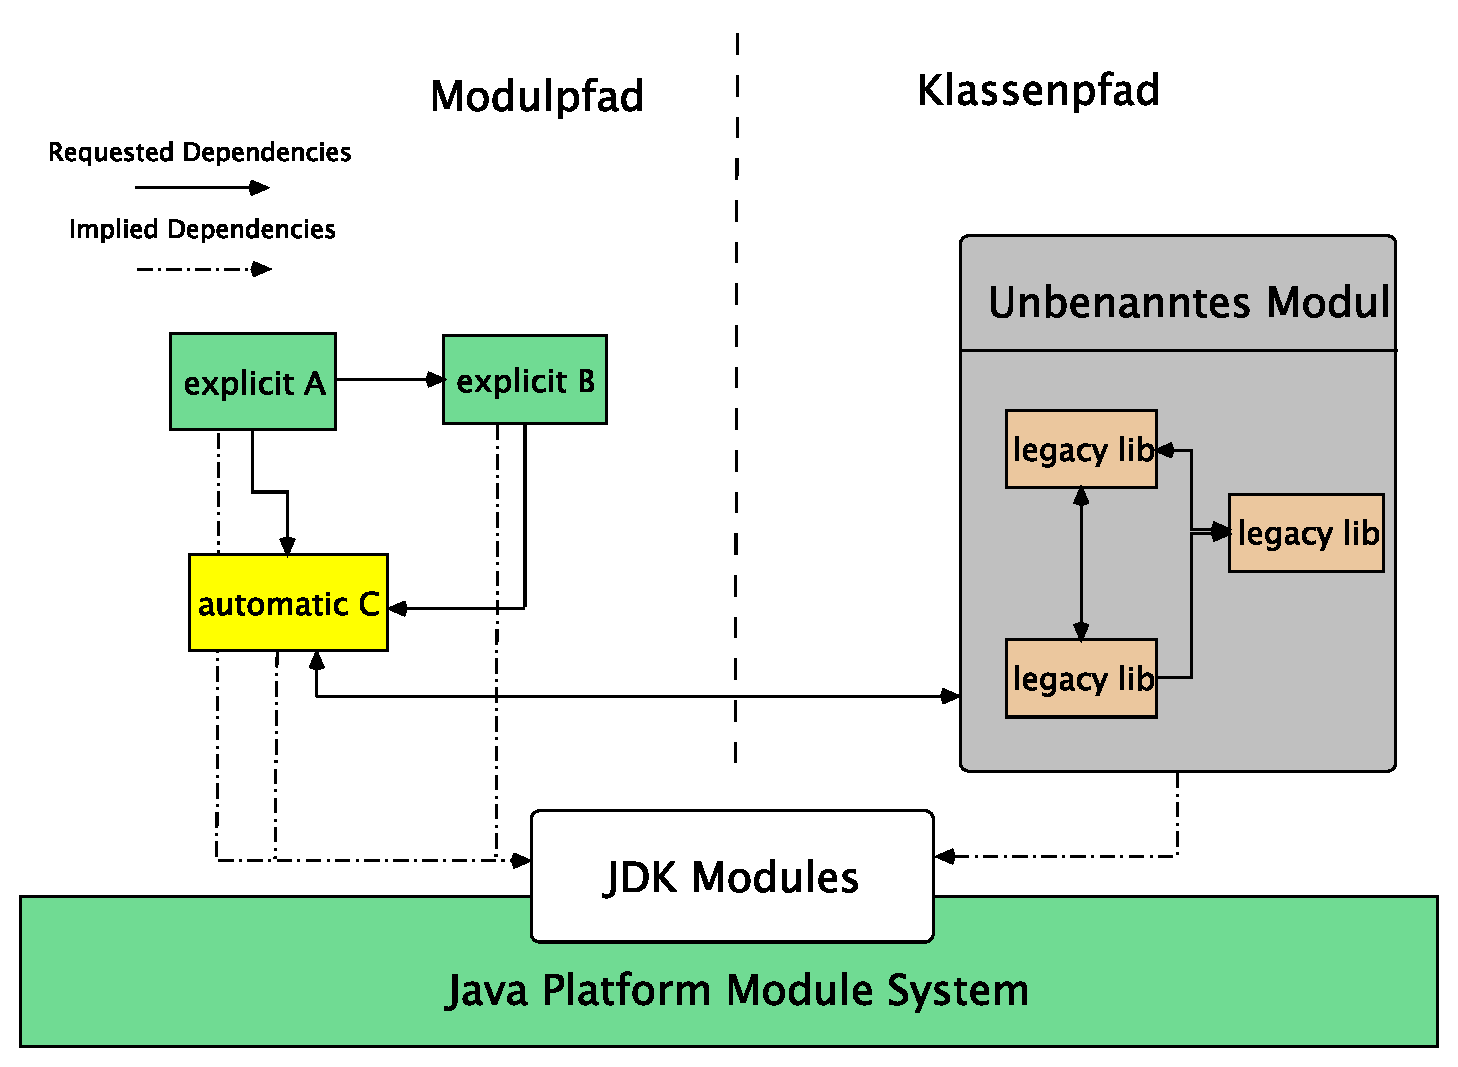
\includegraphics[width=0.8\textwidth]{material/images/top-down-migrate.pdf}
	    \caption{\textit{Top Down} Migration}
	    \label{fig:TDM}
  	\end{figure}

	Diese Migration ist besonders vorteilhaft bei Applikationen, die eine geringe Codebasis besitzen und in einem kurzen Zeitraum eine modularisierte Form annehmen können. 

\subsection{Bottom Up Migration} \label{sec:bottomUP}
	Die \textit{Bottom Up} Migration behandelt lose Module zuerst, denn diese haben keine Abhängigkeiten und bieten eine gekapselte Funktionalität an. Um herauszufinden, welche Module sich für den initialen Migrationsschritt eignen, kann der Abhängigkeitsgraph mithilfe des \textit{JDepth} erstellt werden. Module, die als Blätter aufzufinden sind, können zuerst migriert werden, da sie keine Kinderknoten und somit keine Abhängigkeiten besitzen. Im weiteren Verlauf der Migration werden die übrig gebliebenen und neu entstandenen Blätter des Abhängigkeitsbaums abgearbeitet, bis die ganze Applikation, samt der Drittanbieter Bibliotheken, sich auf dem Modulpfad befindet. Während der Migration müssen natürlich die im Kapitel \ref{sec:MEK} besprochenen Kriterien erfüllt werden, um eine robuste Umsetzung zu erreichen. \cite{javaMod9,modulProgJava9,java9modRevealed,modulMitJava9,masteringJava9} \bigbreak
	\begin{figure}[h]
		\centering
	    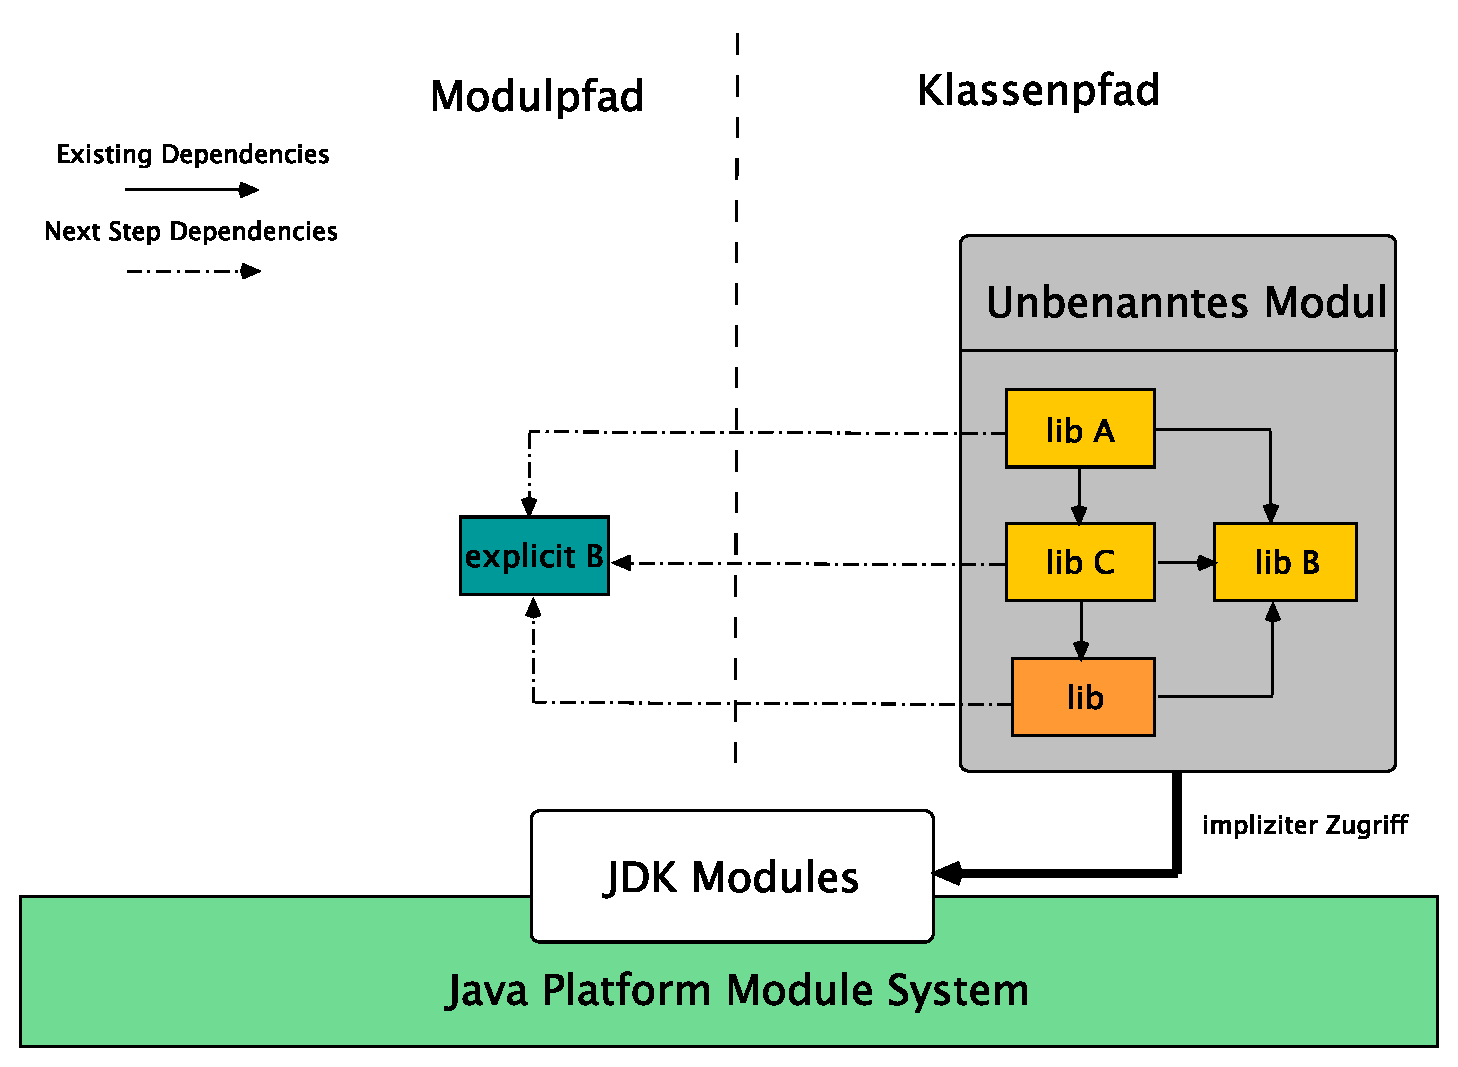
\includegraphics[width=0.8\textwidth]{material/images/bottom-up-migrate.pdf}
	    \caption{\textit{Bottom Up} Migration \cite{modulMitJava9}}
	    \label{fig:BUM}
  	\end{figure}
	In der Abbildung \ref{fig:BUM} wird der erste Schritt der \textit{Bottom Up} Migration angedeutet, indem die \textit{lib B} als erste auf den Modulpfad migriert wird. Diese hat keine Abhängigkeiten und ist der perfekte Kandidat für den initialen Schritt. Als Nächstes bietet sich die \textit{lib} Bibliothek für die Migration an, da sie keine weiteren Abhängigkeiten in den Klassenpfad besitzt. Jedoch ist sie eine Drittanbieter Bibliothek und kann von uns nicht bearbeitet werden. Aufgrund dessen wird die \textit{lib C} für  den nächsten Migrationsschritt ausgewählt und als ein \textit{automatisches Modul} auf den Modulpfad migriert. Somit kann dieses die \textit{lib} und \textit{lib B} zugleich nutzen. Als Nächstes ist die \textit{lib A} an der Reihe, dessen komplette Abhängigkeiten sich bereits auf dem Modulpfad befinden. In der Konsequenz befinden sich alle Applikationsbibliotheken auf dem Modulpfad. \cite{javaMod9,modulProgJava9,java9modRevealed,modulMitJava9,masteringJava9} \bigbreak

	Die \textit{Bottom Up} Migration bietet sich bei bereits aufgeteilten Applikationsarchitektur an, die über eine Menge von \textit{Jar} Bibliotheken betrieben wird. Diese braucht weniger Aufwand, um den Monolithen zu zerlegen und sind bereits über Schnittstellen miteinander Verbunden. \cite{modulProgJava9,modulMitJava9}









\chapter{Analyse der Ausgangssituation} \label{cha:ausgangssituation}
	Dieses Kapitel diskutiert die Motivation für die Abschlussarbeit, setzt klare Ziele sowie Rahmenbedingungen und erörtert den Einfluss des Java Modulsystems auf \textsc{Renew} wie auch die derzeitige Plugin-Architektur. Des Weiteren wird ein Zustand ermittelt, der als Basis für die nachfolgenden Prototypen gelten wird.

\section{Motivation}\label{sec:motivation2}
	\textsc{Renew} ist ein Petrinetz Simulator, der von dem Arbeitsbereichs TGI/ART entwickelt wird und unterstützt das Erforschen von komplexen Systemen auf der Grundlage formaler Modelle.\newline
	Weil \textsc{Renew} in Java geschrieben ist, ist die Applikation an die Java Plattform angewiesen und muss dementsprechend den Plattformanforderungen und Richtlinien folgen. Die Anforderungen und Richtlinien einer Plattform sind nicht festgelegt und können sich ändern, besonders mit einem großen Versionssprung. Das neu eingeführte Modulsystem von Java, wird mit einem großen Versionssprung in Verbindern gebracht und setzt neue Normen und Anforderungen für die Entwicklung von Java Applikationen. \bigbreak
	
	Es gibt mehrere Gründe warum \textsc{Renew} die Migration auf das Modulsystem durchführen sollte. Im Folgenden werden die wesentlichen Argumente, die für die Migration sprechen diskutiert.  

	\subsection{Evolution der Plugin-Architektur} \label{sub:architektur}
		Die initiale Entwicklung von \textsc{Renew} begann miteiner monolithischen Architektur. Diese erfüllte die nötigen Anforderungen, eignet sich jedoch nicht für Entwickler mit geringer Kenntnis über die Gesamtarchitektur und den darunterliegenden Konzepten. Daher wurde eine Plugin-Architektur aufgesetzt, die es ermöglichte Studenten \textsc{Renew} mit Logik innerhalb eines Plugins zu erweitern. Dieses Verfahren trägt bereits den Gedanken der Modularisierung in sich, da die Gesamtarchitektur in Bestandsteile zerlegt und miteinander entkoppelt verknüpft wird. Somit wäre die Einführung des Modulsystems von Java der nächste Schritt in Richtung erweiterbare und zusammensetzbare Systeme.

	\subsection{Parallele und Verteilte Entwicklung}\label{sub:vez}
		Die Aufteilung einer monolithischen Architektur auf eine Plugin-Architektur war ein großes Ereignis für Renew. Denn mit der Zerlegung der Gesamtarchitektur wurde die Komplexität auf die entstandenen Komponenten aufgeteilt und erlaubte eine mühelose Weiterentwicklung der Applikation über die Plugins. \bigbreak

		Obwohl die \textsc{Renew} Plugin-Architektur lange im Betrieb blieb, hatte das Plugin-System die Codebasis umorganisiert, ohne diese zu verändern. Diese führt zu altem, unverständlichem Code aus der Java 1.4 (2002) Version, mit dem viele Konzepte und Architektur Entscheidungen getroffen wurden. Nach fast 18 Jahren Betrieb altert die Codebasis, die Ideen und Konzepte für die Umsetzung ihrer Funktionalität. Besonders konfus und aufgebläht können Funktionsumsetzungen erscheinen, die heute von Java 12 in ein paar Zeilen gelöst werden können. Der zügige und rapide Wandel der Software Paradigmen und deren optimaler Einsatz in der Software Architektur ist ein Teil des Fortschritts und muss in die Planung des Lebenszyklus der Applikation mit einkalkuliert werden. \newline
		Dementsprechend ist die Modularisierung und dessen Anforderung an die Struktur und Inhalt ein wichtiges Ereignis für den \textsc{Renew} Lebenszyklus. Denn dieser erreicht wieder sein Ende und wird mit dem Modularisierungsschritt zurückgesetzt. \bigbreak

		\textsc{Renew}'s Entwicklungseinheit ist das Plugin. Diese repräsentiert ein bestimmtes Feature mit einem eigenen Lebenszyklus, wie zum Beispiel ein Formalismus, Simulator oder Fenster Management Plugin. Diese müssen Daten entgegennehmen, diese verarbeiten und wieder ausgeben. Demzufolge bündelt ein Plugin mehrere Fähigkeiten, die zusammen ein Feature verkörpern. Der wesentliche Nachteil einer Codeänderungen in einem größeren Plugin, ist das Beeinträchtigen des Gesamtverhaltens des Plugins und fordert dementsprechend ein komplettes Testszenario aller Plugin Fähigkeiten.\newline
		Mit der Einführung der Module, kann das Plugin in kleinere Einheiten zerlegt werden, die anschließend eine gekapselte Teilfunktionalität des Plugins in sich tragen und Auswirkungen der Modifikation eingrenzen. Diese sind klein, leicht änderbar, ersetzbar und besitzen einen eigenen unabhängigen Lebenszyklus. Somit verkürzt sich die Entwicklungsdauer einer Änderung innerhalb eines Plugins, da der Einfluss auf die Umgebung durch die Modulgenerzen eingeschränkt ist. Des Weiteren  bieten Module eine Möglichkeit kooperativ und parallel an einem Plugin zu arbeiten, indem die Module gegen vereinbarte Schnittstellenbeschreibungen entwickelt werden. \bigbreak

		Demnach erweitert die Modularisierung den \textsc{Renew} Kontext und erlaubt das Entwickeln von Plugins in Rahmen eines Studenten Projekts, indem Teilaufgaben eines Plugins auf Module zerlegt und parallel von Studenten bearbeitet werden können. Darüber hinaus ist das Zusammenführen der Ergebnisse eine konfliktfreie Angelegenheit und bedarf keiner kompletten Gruppenaufmerksamkeit, um die passenden Codeblöcke für die Gesamtfunktionalität auszuwählen, da es sich so gut wie keine Überschneidung in der Aufgaben Implementation bilden kann. Somit profitiert \textsc{Renew} von den kurzen Entwicklungszyklen der Module und deren unproblematischen Verknüpfungseigenschaften. 

	\subsection{Kommutative Code-Bausteine}\label{sub:cbs}
		Eine der wichtigsten Fähigkeiten eines Entwicklers, ist die Beherrschung der Komplexität. Diese führt zu sauberem, lesbarem, wartbarem Code und erweitert den Lebenszyklus einer Software um ein Vielfaches. Um diese Kompetenz zu meistern, bietet das Modulsystem von Java unterstützende Werkzeuge, die den erstellten Code organisieren und strukturieren, um ein langlebiges Ergebnis zu erzielen.\bigbreak

		Da \textsc{Renew} das Produkt vieler Abschluss-, Projekt- und Promotionsarbeiten ist, durch die die Software ihre Gestalt annimmt, gibt es diverse Beschäftigte mit eigenen Zielen und Interessen. Daher ist eine allgegenwärtige, globale Strukturanforderung, die jedem Entwickler bekannt ist und die verpflichtend eingehalten werden muss, eine erstrebenswerte Charakteristik.\bigbreak

		Die im Kapitel \ref{cha:modularisierung} vorgestellten Modul Charakteristiken beschreiben die von dem Java Modulsystem eingesetzten Richtlinien für die saubere Softwareentwicklung und erzwingen zum Teil ein Still der fein granulierten Code-Bestandteile, die kombiniert ein Softwaresystem ergeben.\newline
		Die Charakteristiken fördern den Entwickler zum Entwickeln von abgeschlossen Einheiten auf und verhindern somit das Entstehen von den sogenannten \textit{Spaghetti Code}, der funktionsübergreifende Anpassungen trifft und den Überblick über den Zusammenhang der Gesamtarchitektur unscharf erscheinen lässt. \bigbreak

		Die Module und die entsprechenden Richtlinien erschweren den \textit{Spaghetti Code}, indem Mehraufwand für die Kommunikation zwischen den Modulen erbracht werden muss und machen das unsaubere Arbeiten unattraktiv. Somit dienen Module als Grenzen für den Entwicklungsrahmen eines Features und engen den Bearbeitungs- und Betrachtungsraum für den Entwickler ein. Daraus ergibt sich ein Softwarepaket, das unabhängig von den Senior-Entwicklern verstanden, genutzt und angepasst werden kann, da der Aufbau nicht mehr in dem Wiki, Readme oder beim Entwickler selbst verankert, sondern direkt in der Codebasis integriert ist.\bigbreak

		Demzufolge profitiert \textsc{Renew} von der Modularisierung, indem sich immerfort wechselnden Akteure eine saubere Codebasis hinterlassen, die den nächsten Absolventen sowie den wissenschaftlichen Mitarbeitern viel Zeit erspart. \bigbreak

		Aus einer sauberen Umsetzung folgen saubere Code-Bausteine, die wiederverwendet werden können. Die genannten Eigenschaften der Module bringen einen wesentlichen Vorteil beim Optimieren der \textsc{Renew} Applikation, indem kontextbezogen Module ausgetauscht werden können, um ein besseres, lokales Ergebnis zu erzielen. Zum Beispiel können zielgerichtet ausgewählte Plugins für die Erfüllung einer speziellen Aufgabe, wie das Validieren von P/T-Netzen, ein besseres Ergebnis abliefern, indem ein für diesen Anwendungsfall angepasste Verarbeitungsalgorithmus angewandt wird. Dieser ist natürlich in einem Modul gekapselt und besitzt Schnittstein identisch zu seinem Vorgänger. Auf diese Weise kann eine große Anzahl an Modulen mit gleicher Funktion und unterschiedlicher Zielsetzung erstellt werden, die in einem Modulkatalog verwaltet und bei Bedarf ausgetauscht werden können.

	\subsection{Code Management}\label{sub:code_managment}
		Das Plugin Management ist ein zentrales Themengebiet von \textsc{Renew}, da Plugins geladen instanziiert und genutzt werden müssen. Diese wichtige Aufgabe übernimmt der \textit{PluginManger} innerhalb des \textit{Loader}-Plugins, der Plugins in den Klassenpfad lädt und mit den benötigten Bibliotheken ausstattet. Das Laden geschieht über den Plugin-Klassenlader, der den Code aus den gegebenen Quellen auf den Klassenpfad platziert.\bigbreak
		\begin{figure}[t]
		  \centering
		  \includegraphics[width=\textwidth]{material/images/Klassenpfad.pdf}
		  \caption{Klassenpfad Suche \cite{kothagal2017modular}}
		  \label{fig:CP_Struktur}
		\end{figure}
		Der große Nachteil des Klassenpfads ist die Auflösung von Archiv Grenzen und somit auch von Plugin Grenzen. Das heißt, Java kann nicht unterscheiden aus welcher Bibliothek die Klasse stammt und muss aus diesem Grund den kompletten Klassenpfad für eine Plugin Klassenabfrage durchsuchen. Infolgedessen ist das Überwachen der Plugins auf dem Klassenpfad nur schwer möglich, da der Klassenpfad nur Informationen über die Klassen und ihre Pakete besitzt \ref{fig:CP_Struktur}. Des Weiteren ist die Zuordnung einer Klasse zu ihrer Quelle ebenso problematisch.\bigbreak

		Dieses Verfahren wurde ständig bemängelt und wird mit der Einführung des Modulsystems von Java adressiert, indem die Konfigurationsdateien \textit{module-info.java} eingeführt wurde, die der Klassen Quelle eine Identität verleiht. Demzufolge ist ein Archiv oder Verzeichnis nicht mehr ein Aussagen loser Behälter, sondern ein Objekt, das Information über seine Kennung, seinen Inhalt und seiner Kommunikationspartner besitzt.\newline
		Dies bring zwei wesentliche Vorteile für die Arbeit mit dem Plugin Code. Die erste Eigenschaft beschreibt Referenzen auf Archiv-Objekte, die die benötigten Klassen besitzen. Der Klassen werden nicht mehr von links nach rechts durchsucht \ref{fig:CP_Struktur}, wie es vorher der Fall war, sondern über das Modul mit den entsprechenden Klassen adressiert \ref{fig:MP_Struktur}.\cite{kothagal2017modular} \newline
		Das bewusste Nachschlagen nach Klassen erhöht die Performance und setzt zusätzlich das eindeutige und verantwortliche Modul für die gegebene Implementation fest. Darüber hinaus erleichtert die eindeutige Modulzuordnung das Verfolgen von unerwarteten Verhalten, wie zum Beispiel das Überdecken von Klassen von weiteren Klassen desselben Typs, die sich weiter vorne im Klassenpfad befinden.\bigbreak 
		\begin{figure}[h!]
		  \centering
		  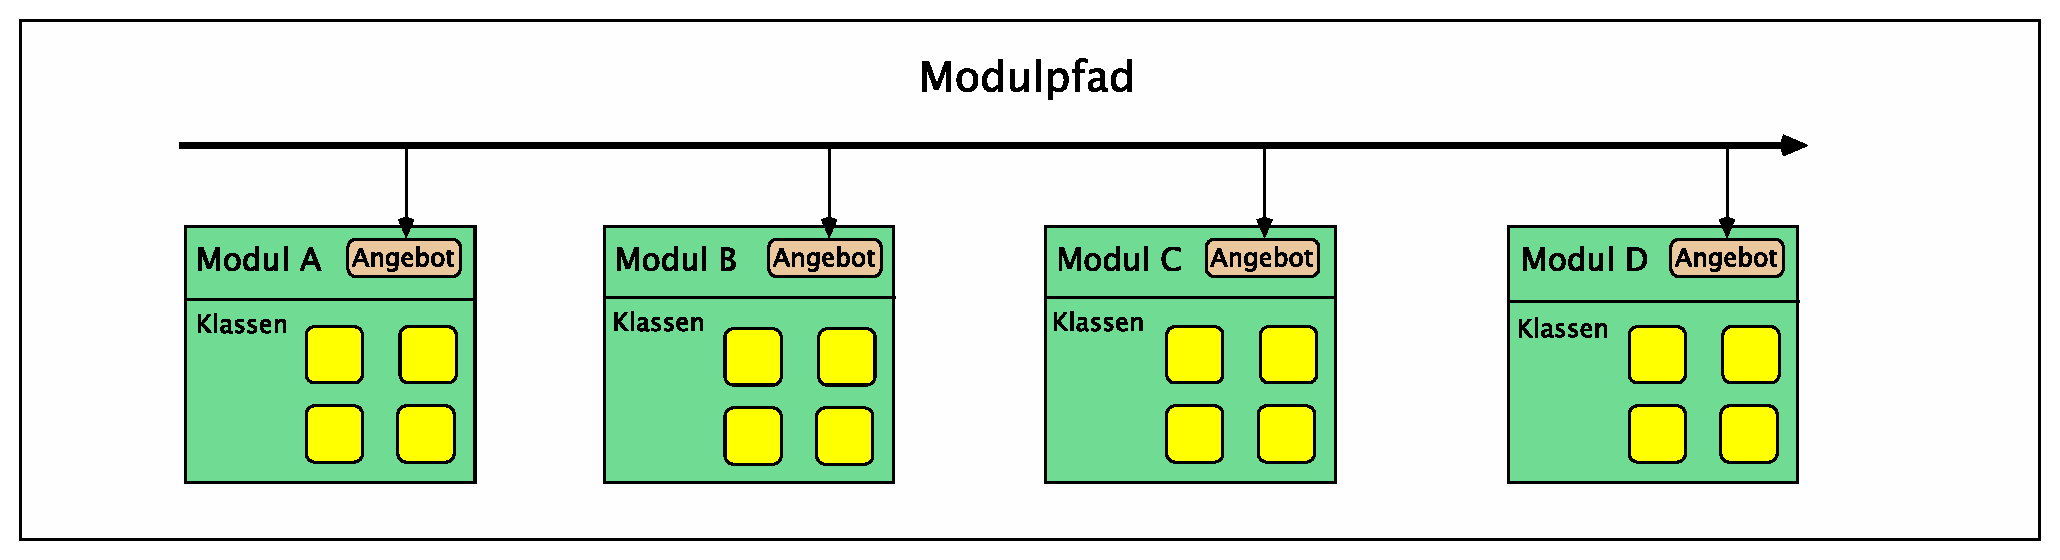
\includegraphics[width=\textwidth]{material/images/Modulpfad.pdf}
		  \caption{Modulpfad Suche}
		  \label{fig:MP_Struktur}
		\end{figure}
		Der zweite Vorteil, beschreibt das Auslesen der Modulinformation aller Module, die sich auf den Modulpfad befinden. Demzufolge können Plugins in Archive verpackt und auf dem Modulpfad wiedergefunden, analysiert und sogar bearbeitet werden. Somit bring Java ein neues Instrument zum Verwalten der Codebasis von modularisierten Anwendungen, die dem Nutzer bei Bedarf die internen Bausteine präsentieren lässt.\bigbreak

		\textsc{Renew} kann mithilfe der neuen API des Modulsystems die Verwaltung der Plugins erweitern, indem geladenen Plugins direkt angesprochen und manipuliert werden. Zum Beispiel könnten auserwählte Plugins nur für bestimmte Nutzer oder Modi ihre Funktionalität anbieten oder eine angenehme Visualisierung der laufenden Plugins und dazugehörige Funktionalitäten dem Nutzer präsentieren. Des Weiteren ist die performante Suche nach Klassen in einem dynamischen System wie \textsc{Renew}, eine erstrebenswerte Qualität.  \newline
		Im folgenden Kapitel der Auswirkungen \ref{sec:auswirkung} wird auf die \textit{Modulschicht} eingegangen, die das zielorientierte Laden nur notwendiger Module und somit nur notwendiger Plugins ermöglicht.

	\subsection{Abgeschlossene Laufzeitabbildung} \label{sub:laufzeit_images}
		Für die Nutzung von Java Applikationen ist immer eine installierte Laufzeitumgebung notwendig, die Versionskompatibel mit der entsprechenden Applikation sein muss. Dementsprechend muss Java installiert und eingerichtet werden bevor unser Code ausgeführt werden kann. Für große Serveranwendungen ist der Aufwand gerechtfertigt, da sie unikale, langlebige und komplexe Gebilde darstellen. Für Anwendungen, die kleiner sind und dynamisch zwischen Hardwareknoten verteilt werden müssen, ist das manuelle Anlegen der Laufzeitumgebung eine mühselige und fehleranfällige Aufgabe. \newline
		Das Modulsystem von Java hat diese Herausforderung mithilfe der \textit{Laufzeitabbildung} adressiert. Die \textit{Laufzeitabbildung} besteht aus einer Verzeichnisstruktur, die alle notwendigen Komponenten für den Betrieb der Applikation besitzt. Dazu zählen Module, Skripte, native Bibliotheken, Konfigurationen, Dokumentationen sowie Lizenzbedingungen und sogar Sicherheitsmechanismen zum Validieren der Komponenten sind vorgesehen. Die generierten \textit{Laufzeitabbildungen} sind in sich Abgeschlossen und können einfach auf beliebig viele Hardwareknoten automatisiert verteilt und ausgeführt werden, ohne zusätzliche Justierung der Software Umgebung. \bigbreak
		Die Eigenschaft der Abgeschlossenheit der \textit{Laufzeitabbildung}, kann von \textsc{Renew} aufgegriffen und genutzt werden, um ausgewählte Plugin Gruppen horizontal nach Belieben zu skalieren. Zusätzlich hält die \textit{Laufzeitabbildung} nur notwendige Java sowie Benutzer erstellte Module, die bestens für die Ausführung der Applikation aufeinander abgestimmt werden. Infolgedessen kann das modularisierte \textsc{Renew} auf optimale Ausführungsgeschwindigkeiten zählen. 

	\subsection{Integration in moderne Technologien} \label{sub:moderner_zustand}
		% Ziel
		Der zeitgemäße Zustand einer Applikation ist ein Zeichen hoher Qualität und reflektiert enorme Ansprüche an den Betrieb der Applikation. Diese kann geschäftskritische Qualitäten tragen, die den marktführenden Vorteil bringt und der Konkurrenz ein Schritt voraus ist. Um den Vorsprung zu sichern, ist eine vorausschauende Flexibilität gefragt. Mithilfe dessen die Applikation in der Lage ist, mit minimalem Aufwand, an die führenden Technologien anzuknüpfen.

		% Trends 
		Die aktuell führenden Trends beschäftigen sich mit der verteilten und wiederverwendbaren Softwareumsetzungen, die ständig an Komplexität gewinnen und trotzdem leicht beherrschbar bleiben muss. Diese beschreiben Ansätze wie gewisse Ziele erreicht werden können und setzen Grundvoraussetzungen zum Erreichen dieser Ziele. Dementsprechend muss \textsc{Renew} bestimmte Grundvoraussetzungen erfüllen, um die Vorteile der Trends zu Nutzen und den Schritt mit dem Fortschritt zu halten.  \bigbreak

		% Docker  
		Zum Beispiel wäre die Docker Umgebung für \textsc{Renew} eine willkommene Erweiterung, mit der interne Bestandsteile distributiv betrieben werden können. Somit wäre die Ausführung von \textsc{Renew} nicht mehr an eine Maschine gebunden und kann bei Bedarf horizontal skaliert werden. Im Folgenden stellt sich die Frage: Welche internen Strukturen von \textsc{Renew} müssen individuell behandelt und anschließend kooperativ zusammengeführt werden. Auf diese Frage gibt es keine pauschale Antwort, jedoch ist es klar, dass die Plugins von \textsc{Renew} feingranular betrachtet werden müssen, um sich ein Bild der Verarbeitungskette zu erstellen und diese den Bedürfnissen anzupassen. \bigbreak

		% Microservice  
		\textsc{Renew} auf verschieden Hardwareknoten zu verteilen ist nur der erste Schritt der distributiven Ausführung. Es fehlt die Koordination zwischen den Knoten, die die Verarbeitung koordinieren und die Ergebnisse zusammenfassen. Somit gibt es eine weitere Technologie, die sich dieser Aufgabenstellung widmet: Der Mikroservice Architekturansatz, der sich um die Koordination und das Zusammenspiel von Applikationsschwärmen kümmert. \bigbreak

		% Fazit 	
		Mithilfe der Mikroservicearchitektur und der Docker-Umgebung wäre die distributive Ausführung von \textsc{Renew} erreichbar, doch zuerst muss \textsc{Renew} den aktuellen Stand der Technologie entsprechen und demzufolge das Modulsystem von Java integrieren.  		
		
\section{Anforderungsanalyse} 
	Indem der Java-JDK mit der neunten Version von Java modularisiert wurde, ändern sich die grundsätzlichen Funktionsrichtlinien der Plattform, die Konsequenzen für bestehende Systeme mit sich bringen. Denn das Modulsystem von Java führt eine obligatorische Kapselung der Code-Komponenten ein, die über erweiterte Sicherheitsmechanismen verfügen und nur über explizite Schnittstellen geladen und angesprochen werden können.\newline 
	Diese Abschlussarbeit beschäftigt sich mit der Untersuchung von Anforderungen der modularisierten Java Plattform, sowie dem entsprechenden Aufwand für das Anpassen bestehender Systeme. Darüber hinaus sollen die neu eingeführten Java Konzepte für den Einsatz im Rahmen der dynamischen Systeme untersucht werden.\newline
	Für die Umsetzung muss ein grundlegendes Migrationsverfahren erarbeitet und angewandt werden, welches eine Migration auf das Modulsystem von Java ermöglicht. Da die Migration bestehender Systeme nicht in einem Schritt durchgeführt werden kann, müssen Charakteristika für Module formuliert werden, um bestehende Systemelemente innerhalb einer ausgereiften Software mit den entsprechenden Eigenschaften zu erweitern.\newline
	Jede kleine Änderung in einem komplexen System bringt große Risiken mit sich, die das saubere Arbeiten der Software infrage gestellt. Daher ist der Übergang auf das Modulsystem von Java mit Unsicherheit verbunden, zumal es Zeit kostet, im Code verankertes Geschäftswissen umstrukturiert und keine sichtbare Softwareerweiterung für den Endkunden darstellt. Demnach liegen die Schwerpunkte der Migration in der Konsistenz der gegebenen Software im neuen Kontext, dem Mehrwert sowie in dem Aufwand der Umsetzung. \newline
	Die Erarbeitung der neu eingeführten Java Konzepte muss den Mehrwert für den Einsatz im dynamischen System abbilden und einen möglichen Einsatz darstellen.

	Um die gegebenen Anforderungen an eine Applikation zu stellen, bedarf es einer passenden Projektstruktur und Umsetzungswerkzeuge, die eine Modulmenge kompilieren und verpacken. Zu diesem Zweck soll das Java basierte Gradle Werkzeug eingeführt werden, das eine kompakte und mächtige Ausdrucksform für das Erstellen von Softwaresystemen Entwicklungsumgebung unabhängig anbietet. \bigbreak

	Für die Umsetzung der erarbeiteten Konzepte steht der \textsc{Renew} Simulator und das \textsc{Mulan} Rahmenwerk zur Verfügung, die in dieser Abschlussarbeit Migrationsszenarien erleben.\newline 
	Das erste Szenario soll eine kontinuierliche Migration einer Software auf das Modulsystem modellieren. Im Gegensatz dazu wird im zweiten Szenario alt Software auf eine modularisierte Codebasis aufgesetzt und der parallele Betrieb begutachtet. 

\section{Anforderungsspezifikation} 
	Für den Anwendungskontext der Modularisierung einer größeren Anwendung steht \textsc{Renew} und \textsc{Mulan} zur Verfügung, jedoch übersteigern eine vollwertige Modularisierung von \textsc{Renew} und \textsc{Mulan} den Zeitrahmen dieser Abschlussarbeit, da die Umstellung jedes einzelnen Plugins auf organisierte Modulverbände eine zeitintensive Aufgabe verkörpert. Jedes einzelne Plugin muss analysiert, reorganisiert, auf Module zerlegt und bestens miteinander verzahnt werden. Darüber hinaus müssen die entstandenen Module mit allen gegenwärtigen Plugins abgestimmt werden, da das Plugin Modulverband generell andere Schnittstellen anbieten wird. \bigbreak
	Dementsprechend wird die Modularisierung auf einzelne Plugins reduziert, die für die Darstellung der UI sowie die grundsätzliche darunterliegende Logik zuständig sind. Um die Kommunikation im bestehenden System zu garantieren, behalten die entstandenen modularisierten Plugins ihre Schnittstellen. Infolgedessen wird die Funktionalität aller Plugins nicht beeinträchtigt und garantiert dem Gesamtsystem einen nahtlosen Übergang auf den Modulpfad. Hierfür werden die Plugin Module mit den entsprechenden Konfigurationsdateien erweitert und mit den notwendigen Plugins verzahnt. In der Konsequenz wird die Umsetzung nur die minimalen Anforderungen des Modulsystems realisieren und das Zerlegen der internen Struktur der Plugins aus der Sicht lassen, obwohl es ein wünschenswerter Schritt in Richtung der Modularisierung wäre. \newline 
	Trotz allem müssen die Plugin Projekte von \textsc{Renew} zusätzliche Module unterstützen und die Möglichkeit bieten, \textsc{Renew} zu erweitern, um weitere Module innerhalb eines Plugins erstellen zu können. Dafür benötigen alle Plugins eine neue Projektstruktur, die das gewünschte Verhalten umsetzt und die empfohlene Modulorganisation unterstützt. Dieses trägt die Maven konforme Projektstruktur, die Java Klassen, Ressourcen und sonstige Artefakte nach einem standardisierten Muster verwaltet.\newline
	Für den Einsatz von neu eingeführten Java Konzepten wird ein Grundriss aufgezogen, der eine möglichen Umsetzung der dynamischen Plugin-Verwaltung anbietet. \bigbreak

	Des Weiteren muss die Konfiguration des Projektes von der Entwicklungsumgebung gelöst werden, um den Entwickler nicht in seinem Arbeitsablauf einzuschränken und die Entwicklungsumgebung seiner Wahl zu nutzen zu dürfen. Dazu soll die existierende Ant Umgebung mit Gradle ersetzt werden. Diese erleichtert das Verwalten sowie Verpacken der Software und verspricht zusätzlich eine kohärente Arbeitsweise mit dem Modulsystem von Java, indem das Verwalten der Modulabhängigkeiten sich in beiden Systemen widerspiegeln. Diese Eigenschaft soll auf die modularisierte Version von \textsc{Renew} angewandt und evaluiert werden. \bigbreak

	Da der \textsc{Renew} Simulator von verschiedenen Abschlussarbeiten beleuchtet und erweitert wird, beinhaltete die Applikation verschiedene Techniken der Softwareentwicklung, wie zum Beispiel das Generieren von Java Klassen mit dem \textit{JavaCC} Compiler. Dementsprechend existieren ältere Verfahren innerhalb von \textsc{Renew}, die sorgfältig auf Kompatibilität mit der neuen Umgebung untersucht und migriert oder ersetzt werden müssen. \bigbreak
	Das Aufbereiten der Grundlagen sowie der Ausgangssituation sind essenzielle Schritte einer Migration, da diese das Fundament für die Planung und Umsetzung legen. Zusätzlich leitet die Ausgangssituation das Migrationsszenario, das eine beispielhafte Schrittweise Migration oder Integration demonstriert und evaluiert.\bigbreak

\section{Auswirkung von Gradle und JPMS auf \textsc{Renew}} \label{sec:auswirkung}
	Die Folgeerscheinung der Modularisierung unterbindet zahlreiche Entwicklungsschwächen, wie die \textit{Codeorganisation}, \textit{Zyklen}, \textit{Split Packages} und antiquierte API's. Diese sollen mit der Migration auf das Modulsystem von Java aufgelöst, reorganisiert und nachgerüstet werden, um einen kompilierfähigen Zustand erreichen zu können.

	\subsection{Projektstruktur} \label{sub:projektstrukutr}
		Das Plugin System von \textsc{Renew} besteht aus einer großen Anzahl an Plugins, die Zweckorienttier kombiniert werden können. Demnach besteht bereits ein Organisationsaufwand, der mit jeder Plugin Kombination wächst. \bigbreak

		Zu den bestehenden Organisationsaufwand wird eine neue Ebene der Administration eingeführt, nämlich die Ebene der Module. Diese zerlegen Aufgabenmengen aus einer Code-Struktur in mehrere Code-Bausteine, die infolgedessen innerhalb eines Plugins disjunkt verwaltet werden müssen.\newline
		Da die Kombination aus Plugins und Modulen ausschlaggebend für die \textsc{Renew} Funktionalität ist, muss eine passende Projektorganisation eingerichtet werden, die jedem Plugin die Möglichkeit bietet, zusätzliche Module mit dem Quell-Code, den Ressourcen sowie den Tests anzulegen.\bigbreak

		Des Weiteren spielt die Paketorganisation eine zunehmend stärkere Rolle im Modulsystem von Java, denn eine Überschneidung eines Paketnamens mit anderen Bibliotheken im System ist ausgeschlossen und muss dementsprechend einen global eindeutigen Namen besitzen. \newline
		Die Einschränkung in der Namensgebung und Code Organisation ist für \textsc{Renew} eine substantielle Änderung. Die Plugins wurden von unterschiedlichen Entwicklern zu unterschiedlichen Zeitpunkten entwickelt, ohne eine einheitliche Struktur Plugin übergreifend einzuhalten. Daraus folgt eine wilde Ressourcen- und Java Fremdcode Allokation, die das Lesen, Analysieren und bearbeiten der Plugins schwierig gestaltet. Zum Beispiel befinden sich gewisse Ressourcen im Plugin Wurzelverzeichnis unter \textit{tools}, \textit{samples}, \textit{ontology} und andere direkt im Java Source-Code unter \textit{src/**/*.(gif|jj|rnw|sns|vm)}. Der Aufbau führt zu der Frage, wie kompatibel ist das Ressourcenlayout mit dem Modulsystem von Java. Denn Ressourcen werden im Modulsystem von Java genauso wie die Java Klassen innerhalb eines Modulpakets gekapselt und verwaltet. Demzufolge kann das Paket \textit{samples} nur einmal in einer Modulmenge existieren, da das Modul global den kompletten Namensraum für sich und seine Ressourcen allokiert. \bigbreak 

		Das Problem der Ressourcenorganisation, kann mithilfe des \textit{META-INF} Verzeichnis gelöst werden, denn das \textit{META-INF} Verzeichnis ist ein besonderes Verzeichnis, das nicht als ein Klassenpaket interpretiert wird und dementsprechend keinen ausführbaren Code enthält. Demzufolge können namensgleiche Ressourcen Verzeichnisstrukturen in unterschiedlichen Modulen denselben Namensraum besetzen und alle benötigten Ressourcen wie Konfigurationsdateien, Bilder und komplexe Darstellungsobjekte enthalten.\bigbreak

	\subsection{Split Packages}
		Im Kapitel \ref{sub:code_managment}  wurde die neue Klassensuche innerhalb des Modulsystems von Java thematisiert. Die Klassensuche ordnet jedes Klassenpaket eindeutig einem Modul zu, um den Klassenpfad durch eine Struktur zu erweitern, die sicher, schnell und eindeutig ist. Für \textsc{Renew} ist die Voraussetzung der eindeutigen Paketbenennung noch nicht erfüllt. Denn \textsc{Renew} besteht aus Plugins, die sich gegenseitig sowohl ergänzen als auch erweitern und neigen dementsprechend zum ähnlichem oder äquivalentem Aufbau. Zum einen geschieht es bedacht, um zusammengehörige Klassen auf dem Klassenpfad näherzubringen und unter einem Paketnamen zu vereinen, zum anderen geschieht es zufällig, da sich der Aufbau gut für die Zielsetzung eignet.\bigbreak

		Die Lösung für den ähnlichen Aufbau ist die Anpassung der Paketstruktur, die eindeutig für jedes Plugin definiert wird. Zum Beispiel müssen Plugins aus dem gleichen Kontext, wie \textit{Navigator} oder \textit{NavigatorGit}, die denselben \textit{de.renew.navigator.*} Namensraum beanspruchen disjunkt aufgebaut und benannt werden, um eine eindeutige Identität zu etablieren. \bigbreak

		Im Gegensatz zum ähnlichen Aufbau, ist das Erweitern von Plugins, indem gleichnamige Paketstrukturen aufgebaut werden, ein komplexes und tief führendes Problem. Wie bereits im Kapitel \ref{sub:projektstrukutr} besprochen, darf es keine Überschneidung der Namensräume geben. Das heißt, die  Annahme, dass die benötigten Klassen aus anderen Plugins sich in demselben Paket auf dem Klassenpfad befinden ist nicht mehr zutreffend. \newline
		Für \textsc{Renew} hat es eine ganz besondere Bedeutung, da der Code nicht nur kompiliert, sondern zuvor generiert werden muss. Das Generieren geschieht mit unterschiedlichen Techniken, die zum Beispiel mit \textit{rnw, sns, jj, mv} Dateiformaten arbeiten und für bestimmte Anwendungsfälle unterschiedliche Java Klassen sowie Ressourcen generieren. \newline
		Der generierte Code und die generierten Ressourcen orientiert sich auf das Zielpaket und nutzt zum Teil keine \textit{imports}, sondern direkte Klassen Zugriffe, da man sich sicher ist, dass die benötigten Klassen von anderen Plugins innerhalb ihres Pakets nachgeladen werden. Dementsprechend liegt das Problem nicht in der Java Klasse, Ressource oder dem Plugin, sondern in der Verarbeitungskette der Generatoren, die variable Java Klassen sowie dazu passende Ressourcen für die Kompilation bereitstellen. \bigbreak

		Um die \textit{Split Packages} aufzulösen, müssen die Verarbeitungsketten von vorne bis hinten Analysiert und angepasst werden. Dazu zählt das Auffinden der benötigten Java Klassen innerhalb der modularisierten Plugin Menge, das Verweisen auf den vollwertigen Klassennamen sowie das Öffnen und Konsumieren der entsprechenden Pakete aus den notwendigen Plugins. Des Weiteren muss der Anwender der Ressourcen den vollen Zugriff auf alle in der Ressource referenzierten Klassen besitzen, um dessen Inhalt vollständig darstellen zu können. In der Konsequenz ist das Konvertieren der \textit{Split Packages} Technik auf eindeutige Modulstrukturen eine verwurzelte Problematik. \bigbreak

		Das Einsetzen der \textit{Split Packages}, ermöglichte den Entwickler eine einfache Art und Weise Code aus unterschiedlichen Plugins zusammenzuführen. Jedoch hat sich die Technik auf lange Sicht nicht bewährt und wird mit dem Modulsystem von Java verworfen. Da \textsc{Renew} über einen langen Lebenszyklus verfügt und diese Technik von Beginn an weitgreifend einsetzte, müssen diese Mängel behoben werden bevor die Applikation auf den Modulpfad einsatzbereit ist. 

	\subsection{Projektverwaltung} \label{sub:projekt_verwaltung} % gradle tiefer erklären 
		Die Herausforderung dynamische Modulkombination aus einer großen Modulmenge zu erstellen, spielt eine zentrale Rolle in einem Modulverband. Dementsprechend ist die Administration ein wichtiges Instrument für das Entwickeln von modularem Code.\newline
		Für die Verwaltung der Codebasis existieren bereits Werkzeuge, die eingesetzt werden können wie zum Beispiel \textit{Ant}, \textit{Maven} und \textit{Gradle}. Da \textit{Ant} in \textsc{Renew} eingesetzt wird und \textit{Gradle} im Gegensatz zu \textit{Ant} weiterführende Konzepte mit sich bringt, werden  folgend Gründe für den Umstieg von \textit{Ant} auf \textit{Gradle} formuliert.
	
		\subsubsection{Ant}	% ant problem 
		Zurzeit wird \textit{Ant} für das Kompilieren und Erstellen der ausführbaren Plugins Archiven in \textsc{Renew} benutzt. \textit{Ant} ist das älteste der vorgestellten Werkzeuge und setzt die Grundlage für alle nachfolgenden Verwaltungsinstrumente. Dieses ist imperative und teilt dem System mit, was getan werden muss und wie die Arbeit verrichten werden soll. Mit anderen Worten, es wird eine Reihe von Aktionsanweisungen bereitgestellt, die das System in derselben Reihenfolge ausführt. Dementsprechend ist \textit{Ant} höchst flexibel und erlaubt eine feingranulare Konfiguration jedes einzelnen Ausführungsschritts. Wie zum Beispiel das Setzen der Ortsangaben, das Aufteilen sowie das Koordinieren der ausführbaren Code-Menge und natürlich die Kalibrierung des Compilers für die Übersetzung, die verpflichtend durchgeführt werden muss.\newline 
		Obwohl die explizite Konfiguration viele Möglichkeiten bietet, ist das Schreiben und Konfigurieren an keinen Konventionen oder Strukturen gebunden. Infolgedessen führt die Entwicklung zu riesigen XML-Dateien, die nur schwer zu verstehen und zu warten sind. Des Weiteren ist \textit{Ant} auf die Laufzeitumgebung angewiesen und erwartet bestimmte Bibliotheken und Applikationen auf der Ausführungsmaschine vorinstalliert, wie zum Beispiel \textit{Ant} selbst, \textit{Javacc} und andere Applikationen relevanten Software, die aus dem Klassenpfad erreichbar sein müssen. 

		\subsubsection{Renew und Ant} % Renew ant aufbau 
		Da \textsc{Renew} mit dem \textit{Ant} Werkzeuge verwaltet wird, existieren bereits Skripte mit allen notwendigen Schritten für das Erstellen der \textit{Renew} Plugins. Die Skripte sind in drei Kategorien unterteilt, um die Projektverwaltung in \textsc{Renew} zu etablieren. Zuerst wurden allgemeinen \textit{task} und \textit{target} Skripte eingeführt, die für alle Plugins benötigt werden, um die wiederholenden Konfigurationen zu minimieren. Des Weiteren wird für jedes Plugin ein eigenes Skript mit dem entsprechenden Lebenszyklus eingerichtet, der aus den allgemeinen \textit{tasks}, \textit{targets} und zusätzlichen Plugin bezogenen Aufgaben zusammengesetzt wird und zum Schluss ein ausführbares Ergebnis liefert. Die innovative Idee des Lebenszyklus ähnelt stark der \textit{Maven} Umsetzung, die in der Zukunft mit einem integrierten \textit{out of the box} Ansatz werben wird. Dennoch ist die derzeitige \textit{Ant} Umsetzung der \textsc{Renew} Umgebung detailliert und wiederkehrend. \newline
		Nachdem alle Plugins Konstruktion fähig sind, wird ein globales XML-Skript eingerichtet, das alle Plugin Skripte referenziert und verwaltet. Zum Beispiel zählt dazu das Erstellen von Plugin Zusammenhängen und ihre Bearbeitungsreihenfolge.
		
		\subsubsection{Verwaltung der Drittanbieter-Bibliotheken}% überleitung auf schwächen 
		Obwohl \textit{Ant} das Bauen von Java Applikationen automatisiert, war die Verwaltung der Projektabhängigkeiten nicht ein Teil der Umsetzung. Dementsprechend müssen direkte sowie transitive Projektabhängigkeiten von den Entwicklern mitgeliefert und in die entsprechenden Klassenpfade der auserwählten Projekt- \textit{task} und \textit{targets} konfliktfrei eingebunden werden.\newline
		Die Verwaltung der benötigten Bibliotheken ist mühselig und bedarf eines enormen Verwaltungsaufwands, um alle transitiven Abhängigkeiten aufzulösen und Konflikte zu beseitigen. Die Anforderung der höchst gewünschten Abhängigkeitsverwaltung wurde erst in der nächsten Generation von \textit{Maven} umgesetzt und im Anschluss von einem Tochterprojekt von \textit{Ant} namens \textit{Ivy} übernommen.\newline
		Momentan verwaltet \textsc{Renew} die Drittanbieter Bibliotheken manuell und kann die Organisation der Abhängigkeiten bei Bedarf durch den Familienmitglied \textit{Ivy} verwalten lassen. Dazu muss \textit{Ivy} in einer separaten Konfiguration eingerichtet werden, die wiederum für den allgemeinen Fall und für jedes Plugin erstellt werden muss. Die Konfiguration enthält die benötigten Bibliotheken, den Versionsrahmen sowie Kriterien zum ein- und ausschließen von transitiven Abhängigkeiten. \newline
		Somit erfüllt \textit{Ivy} den Wunsch nach Ordnung und Organisation von Drittanbieter Bibliotheken, jedoch hat diese einen Preis. Die Konfiguration wird in einer separaten XML-Datei verwaltet und gestaltet das Lesen und Nachvollziehen der zusammengeführten Konstruktion von \textit{Ant} und \textit{Ivy} mühselig, denn das Fehlen einer Konvention, der Zuwachs an den XML-Dateien und ihr globaler Zweck sind für den Entwickler nicht sofort ersichtlich.\newline
		Zu diesem Zeitpunkt ist \textit{Ivy} nicht Teil von \textit{Renew}, daher bleibt die Abhängigkeitsverwaltung ein wünschenswertes Feature.

		\subsubsection{Von Ant zu Gradle}% weg von ant über maven zu gradle 
		Wie bereits angedeutet, ist die imperative Konfiguration mit \textit{Ant} unstrukturiert und aufwendig. Aus diesem Grund wurde eine eindeutige Konvention gewünscht, die ein fertiges Gerüst an Ausführungsschritten anbietet und für jeden Entwickler sofort verständlich ist. Der Nachfolger \textit{Apache Maven} hat diese Anforderung erfüllt und führt einen global eindeutigen und integrierten Lebenszyklus ein, der mit Plugins und Ausführungsschritten belegt werden kann. Somit verkörpert \textit{Maven} mit dem \textit{convention over configuration} Ansatz ein fertiges deklaratives Rahmenwerk, das trotz der gewünschten Konvention die angebotene Funktion streng an den Plugin Anbieter bindet und somit das Nachrüsten von zusätzlichen Features einschränkt. Aus diesem Grund war das Bedürfnis nach dem nächsten Nachfolger, der die allgemeingültige Konvention von \textit{Maven} übernimmt und diese mühelos erweitern lässt, groß.\bigbreak
		Die Herausforderung mit einer Konvention zu arbeiten und diese bei Bedarf erweitern zu können, hat sich das \textit{Gradle} Projekt gewidmet und verspricht eine flexible und erweiterbare Konvention zum Erstellen von ausführbaren Bibliotheken.\newline
		Dafür wurde das in \textit{Ant} und \textit{Maven} eingesetzt XML-Format als die einschränkende Schwachstelle eingestuft, denn dieses eignet sich bestens für die Übermittlung von Datenobjekten und dessen Eigenschaften, jedoch für das Schreiben von einfacher Logik werden hunderte Konfigurationszeilen benötigt. Dementsprechend ist das Einführen von zusätzlicher Logik in dem XML-Format nur schwer möglich. Aus diesem Grund verzichtet \textit{Gradle} auf den Einsatz von XML und führt eine Programmiersprache ein, die Logik kompakt definieren lässt und diese mit dem mitgelieferten Ausführungscode problemlos zusammenführen kann. \newline
		Der ausgewählte Kandidat trägt den Namen \textit{Groovy}. \textit{Groovy} ist eine dynamische Programmiersprache, die für der virtuellen Maschine von Java entwickelt worden ist und erlaubt an Ort und Stelle das Erweitern und Manipulieren von Objektverhalten.\newline
		Dementsprechend stellt \textit{Gradle} einen Lebenszyklus zur Verfügung, der mit Funktionalität belegt werden kann und erlaubt zusätzlich das Manipulieren und Erweitern von Verarbeitungsschritten, ohne die Einführung von zusätzlichen Klassen. In der Konsequenz erfüllt \textit{Gradle} die gewünschte Kombination aus Konvention und Flexibilität.
		
		\subsubsection{Abgeschlossenen Build-Umgebung mit Gradle} % wrapper 
		Das Problem der einfachen Manipulation einer gegebenen Ausführungsstruktur war ein wichtiger Beweggrund für die Entwicklung von \textit{Gradle}, dennoch gab es weitere Wünsche, die das Arbeiten mit Fremdcode erleichtern sollen. Zum Beispiel eine Konvention für die Build-Umgebung einer Applikation, die vom Entwickler konfiguriert, veröffentlicht und eine betriebsfähige \textit{out of the box} Routine anbietet. Dieser Wunsch wurde durch den \textit{Gradle-Wrapper} erfüllt, der eine eigene \textit{Gradle} Version mit sich bringt, die im Weiteren für das Nachladen und Platzieren der benötigten Bibliotheken auf dem Klassenpfad kümmert. Somit ist das Laden und Bauen einer Applikation nicht mehr an die lokale Maschine gebunden und benötigt kein Java oder Drittanbieter Werkzeuge für das Erstellen eines ausführbaren Ergebnisses. 

		\subsubsection{Renew und Gradle}
		Zusammengefasst vereinigt \textit{Gradle} das Beste aus \textit{Ant} und \textit{Maven}, wie zum Beispiel die Flexibilität von \textit{Ant}, die Konvention sowie die Bibliotheksverwaltung von \textit{Maven} und erweitert diese durch eine Umgebungskonvention sowie eine adaptive Domäne spezifische Sprache, die das Schreiben von Code sowie das Erweitern und Konfigurieren von Abarbeitungsschritten mühelos gestaltet. Des Weiteren werden mit einer abgeschlossenen Umgebung das Bauen und Nutzen von komplexer Software wesentlich einfacher, denn diese ist präpariert und benötigt keine Intervention des Nutzers. \newline
		Im Folgenden werden Gründe für \textsc{Renew}'s Umstieg auf \textit{Gradle} zusammengefasst.\bigbreak
		\begin{itemize}
			\item \textsc{Renew} kann nun auf einen Lebenszyklus mit allen notwendigen Schritten für die Erstellung einer ausführbaren Java Applikation zugreifen und macht somit die manuelle Erstellung von allgemeiner Schrittsequenz wie Kopieren, Kompilieren und Verpacken aus dem \textit{ant} Verzeichnis überflüssig. 
			\item Die importierten Verarbeitungsketten können individuell beeinflusst und erweitert werden, um maßgeschneiderte Ausführungsschritte zu erstellen oder bestehende Schritte auszubauen. Somit können spezifische und notwendige Schritte, wie zum Beispiel das Generieren von Java Klassen, in den bereits vorkonfigurierten Lebenszyklus unkompliziert an der zweckmäßigen Stelle integriert werden. Somit hält die individuelle Plugin-Konfiguration nur von der Norm abweichende Logik, die das Lesen und Verstehen der Plugin Funktionalität einfach und unproblematisch gestaltet. 
			\item Mit dem \textit{Gradle-Wrapper} lässt sich eine fertige Build-Umgebung erstellen, die alles Notwendige für das Kompilieren von \textsc{Renew} in sich trägt. Somit ist die Installation von \textit{JavaCC}, \textit{Ant}, \textit{Cobertura} und anderer unterstützender Software nicht mehr notwendig.
			\item Die integrierte Abhängigkeitsverwaltung standardisiert die benötigten Drittanbieter Bibliotheken und minimiert den Verwaltungsaufwand für alle Plugins. 
			\item Des Weiteren gewinnt das \textit{Auschecken} von \textsc{Renew} Code an Performance, denn die Drittanbieter Bibliotheken sind nicht mehr Teil des Projekts, sondern werden beim Bauen aus dem Web nachgeladen.
		\end{itemize}
		% bild HVV automat gegenbeispiel 
	\subsection{Plugin Charakteristika} \label{sub:plugin_beschriftung}
		Jedes \textsc{Renew} Plugin bietet eine Funktion an, die in bestimmten Einsatzszenarien genutzt werden kann. Um die Funktion anderer Plugins zu nutzen und eigene Funktion anzubieten, wird bestimmte Informationen erwartet, die den Namen, den Zweck und die Basis des Plugins beschreibt. Die benötigte Information wird in der \textit{plugin.cfg} aufbewahrt und von dem \textsc{Renew} Plugin Manager ausgelesen, um die Plugins in Relation zueinander zu setzen und entsprechend der Aufbaureihenfolge zu instanziieren. \newline	
		Mit der Einführung des Modulsystems können die Plugins in einer Modulrepräsentation betrieben werden. Dementsprechend wird das Plugin mit einer \textit{module-info.java} erweitert, die sich mit der \textit{plugin.cfg} in der Funktionalität überschneidet. Im Folgenden werden die Schwächen der \textit{plugin.cfg} gegenüber der \textit{module-info.java} untersucht und zusammengefasst. 

		\subsubsection{Die Schwäche der Plugin.cfg} \label{sub:die_plugin_cfg}
			% nachteile der pluign.cfg Schnittstellen
			Obwohl die \textit{plugin.cfg} die Beziehung der Plugins untereinander beschreibt, ist diese Informantin lückenhaft, denn der \textit{plugin.cfg} aus der Abbildung \ref{fig:plugin_cfg} fehlt die Information über explizite Schnittstellen des Plugins und dafür ausgelegten Pakete. Die \textit{plugin.cfg} besitzt nur eine Auflistung von Plugin Namen, die für die Ausführung präsent sein müssen. Infolgedessen greift der Entwickler auf Funktionalität zu, die nicht für ihn bestimmte ist und beeinträchtigt somit die Wartbarkeit des Systems. Denn jede Änderung der Plugin Logik, kann zu Fehlern und unerwarteten Verhalten seiner Nutzer führen. \newline
			\begin{figure}[h!]
			  \centering
			  \includegraphics[width=0.6\textwidth]{material/images/cfg.pdf}
			  \caption{Die plugin.cfg}
			  \label{fig:plugin_cfg}
			\end{figure}
			% nachteil Drittanbieter werden nicht mitgezogen 
			Auch wenn die Plugin Abhängigkeit in der \textit{plugin.cfg} existieren, beinhalten die Konfigurationsdatei keine Drittanbieter-Bibliotheken, die ein wichtiger Bestandsteil der Software abbilden. In der Konsequenz kann \textsc{Renew} nicht automatisch nachprüfen, ob alle benötigten Drittanbieter-Bibliotheken integriert und mitgeliefert worden sind, um die Software für die Ausführung zu validieren.\newline
			% nachteile Homogene Umgebung
			Des Weiteren besitzt die \textit{plugin.cfg} ausschließlich der Information über die Laufzeitumgebung, die sich gegenüber der Entwicklungsumgebung unterscheiden kann. Denn die Entwickler arbeiten auf einer bestens eingerichteten Maschine mit allen nötigen Bibliotheken und Abhängigkeit, die in der Zielumgebung zu meist nicht existieren. Um der Diskrepanz des Ausführungskontextes entgegenzuwirken, wird eine Richtlinie benötigt, die den Kontext einer Applikation beschreibt. Leider wird dieses Verhalten nicht von der \textit{plugin.cfg} unterstützt. 

		\subsubsection{Die Stärken der module-info.java} \label{sub:module-info.java}
			%  problemstellung der module-info.java (das und dies war nicht toll und deswegen)
			Die Java Module wurden entwickelt, um die Codebasis beherrschbar, flexibel und austauschbar zu gestalten. Demzufolge verfolgt der Modularisierungsansatz und das Plugin Konzept eine ähnliche Herangehensweise. Der Modularisierungsansatz nutzt die \textit{module-info.java} Konfigurationsdatei, die die Information aus der \textit{plugin.cfg} aufgreift und erweitert. \newline
			\begin{figure}[h!]
			  \centering
			  \includegraphics[width=0.6\textwidth]{material/images/m-info.pdf}
			  \caption{Die module-info.java}
			  \label{fig:module_info}
			\end{figure}

			Der Unterschied zwischen der \textit{module-info.java} und der \textit{plugin.cfg} wird bei der ersten Betrachtung sofort ersichtlich, denn die \textit{module-info.java} schränkt den Zugriffsraum auf das Modul ein, indem nur ausgewählte Schnittstellenpakete geöffnet werden, die darüber hinaus von jedem oder nur von auserwählten Konsumenten genutzt werden können. In der Abbildung \ref{fig:module_info} wird die Funktion des \textit{formalism} Plugins über das Paket \textit{de.renew.formalism.function} für die \textsc{Renew} \textit{misc} und \textit{feature structure} Plugins freigegeben. \newline
			Somit enthält jedes Plugin-Modul einen verpflichtenden Kommunikationsvertrag, mit dem das Modul mit seiner Umgebung kommuniziert.\newline
			Die verpflichtende Eigenschaft ist neu für \textit{Renew}, da die \textit{plugin.cfg} bislang nur eine optionale Beschriftung trägt und Fehler oder Mängel zu einem späten Zeitpunkt ungünstig auftreten lässt. Um dem entgegenzuwirken, greift Java direkt in das Projekt ein und führt die benötigten statischen Analysen durch, bevor die Applikation kompiliert und ausgeführt wird. Die Inspektion ist in Java integriert und stellt sicher, dass alle Abhängigkeiten zur Kompilations- sowie Laufzeit verfügbar sind und keine von diesen einen Zyklus hervorruft.\newline
			Die Validation mit der \textit{plugin.cfg} ist leider nicht möglich, da sie nicht Teil der Java Plattform ist und nur von dem \textsc{Renew} Plugin Manager zur Laufzeit verarbeitet wird. Des Weiteren unterstützt die \textit{module-info.java} transitive und statische Abhängigkeiten, die flexible Modul-Zugriffsrechte für die Nutzung weiterreichen und bestimmte Module für optional deklarieren. Dementsprechend wird der Kontext eines Plugin-Moduls implizit an seine Nutzer weitergereicht und macht das Lesen der benötigten Abhängigkeiten verständlich. Denn die explizite Deklaration jedes benötigten Plugin-Moduls und der dazugehörigen Drittanbieter-Bibliotheken, kann zu hunderten Einträgen führen, die an der Stelle keinen Beitrag zu der Struktur leisten. 

		\subsubsection{Direkter Vergleich} \label{sub:Direkter_Vergleich}
			Im Folgende wird eine Tabelle mit Eigenschaften abgebildet, die Gemeinsamkeiten und Unterschiede der beiden Konfigurationsdatei darstellt.\bigbreak
			% bild vergleich 
			\begin{table}[!h]
			\centering
			\begin{tabular}{l|l}
				\textbf{module-info.java} & \textbf{plugin.cfg} \\
				\hline
				\\[-1em]
				Plugin Abhängigkeiten & Plugin Abhängigkeiten \\
				\\[-1em]
			    Bibliothek Abhängigkeiten & \\
			    \\[-1em]
			    Entwicklung- und Laufzeitanalyse & Laufzeitanalyse \\
			    \\[-1em]
			    Wesentlich & Redundant \\
			    \\[-1em]
			    Funktonangebot & Codeangebot \\
			    \\[-1em]
			    Plattform Verpflichtend & Plattform Optional \\
			    \\[-1em]
			    Einschränkender Zugriff & Offener Zugriff \\
			    \\[-1em]
			    Gekapselt und Eindeutig & Gemischt und Verteilt \\
			    \\[-1em]
			    Integrierte Java Dienste & Renew Dienste \\
			    \\[-1em]
			    Namen & Namen \\
			    \\[-1em]
			    & Beschreibung \\
			    \\[-1em]
			    & Eigenschaften \\
			    \\[-1em]
			    & Version \\
			    \\[-1em]
			    & Einstiegspunkt
			    \\[-1em]
			\end{tabular}
			\end{table}

	\newpage
	
\section{Ausgangssituation} \label{sec:ausgangssituation} 
	In diesem Abschnitt wird die Ausgangssituation für \textsc{Renew} sowie \textsc{Mulan} dargelegt, die als Grundlage für die nachfolgenden Prototypen dienen werden. 

	\subsection{Renew Prototyp} \label{sub:renew}
		\textsc{Renew} ist in mehr als 60 Plugins aufgeteilt, die für sich alleinstehende Projekte repräsentieren. Jedes Projekt besitzt eine \textit{build.xml} und wird mit dem übergeordneten Stamm \textit{build.xml} Script zusammengeführt. Die XML-Scripte werden von dem \textit{Apach Ant} Werkzeug evaluiert, kompiliert und zusammengeführt. Infolgedessen entsteht ein \textit{jar} Archiv für jedes Plugin-Projekt. Diese werden in eine bestimmte Orderstruktur für die Ausführung aufbereitet, die sich aus dem \textit{config, plugins} und \textit{libs} Verzeichnis zusammensetzt. \bigbreak

		Der innere Aufbau jedes Plugins benötigt eine besondere Konfigurationsdatei, nämlich die \textit{plugin.cfg}. Diese beschreibt für die Ausführung nötigen Plugin-Abhängigkeiten und wird von dem internen Plugin-Manager verwaltet, der für die richtige Ordnung beim Laden jedes einzelnen Plugins aus dem \textit{plugins} Verzeichnis sorgt. Somit sind die \textit{plugin.cfg} Dokumente ein guter Startpunkt für die Evaluation einer minimalen und lauffähigen \textsc{Renew} Konfiguration. \bigbreak

		\begin{figure}[h!]
		  \centering
		  \includegraphics[scale=0.457, angle=90]{material/images/renew_plugin_dependencies2.pdf}
		  \caption{Gui Plugin-Abhängigkeiten}
		  \label{fig:plugin_deps}
		\end{figure}

		Für die Evaluation der minimalen Konfiguration starten wir aus dem \textit{Gui}-Plugin und arbeiten uns abwärts der Plugin-Hierarchie der \textit{plugin.cfg's} hinab, bis der komplette Graph aufgebaut ist. \newline

		Die in der Abbildung \ref{fig:plugin_deps} repräsentierten Zusammenhänge reflektieren die von den Entwicklern abgestimmten Laufzeitabhängigkeiten, die einen groben Überblick über die nötigen Plugins verschaffen. Diese können zur Laufzeit alle benötigten Daten und Klassen enthalten, jedoch tragen sie keine Aussage über Abhängigkeiten während der Kompilation. Demgemäß kann zusätzlicher Code sowie Plugins benötigt werden. 

	\subsection{Mulan Prototyp} \label{sub:mulan}
		\textsc{Mulan} \cite{Roelke04} ist ein Multiagenten Rahmenwerk, mit dem Agenten entwickelt und miteinander verbunden werden können. Diese agieren nach eigenem Interesse und verhandeln über Kommunikationskanäle, die von \textsc{Mulan} angeboten werden. Um eine auf \textsc{Mulan} basierende Multi-Agent-Anwendung zu erstellen, müssen zahlreiche Protokollnetze gezeichnet und Wissensbasen erstellt werden, die das Verhalten und die Interaktion von Agenten implementieren. Somit bietet \textsc{Mulan} eine Kommunikationsplattform sowie ein Gerüst für die Umsetzung der darauf aufsetzenden Agenten und dessen Eigenschaften sowie Fähigkeiten, die mit Referenznetzen entworfen werden können. \cite{Cabac10a} \bigbreak

		Das Spiel Settler ist mit \textsc{Mulan} umgesetzt und implementiert somit die Agenten Anforderungen des Multi Agenten Systems. Diese halten Wissensbasen über die Spielregeln und können mit Hilfe der Protokollnetze bestimmte Entscheidungen treffen und Handlungen ausführen. Wie zum Beispiel Straßen bauen oder mit Karten handeln.\bigbreak
		
		\begin{figure}[h!]
		  \centering
		  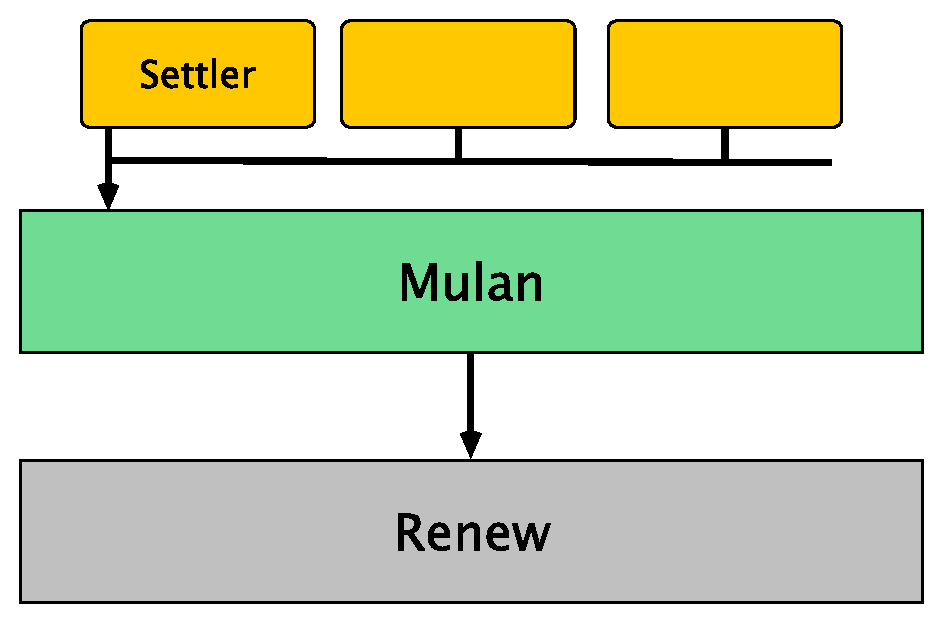
\includegraphics[width=0.5\textwidth]{material/images/settler-mulan-renew.pdf}
		  \caption{\textsc{Mulan} Plugins}
		  \label{fig:mulan_plugin}
		\end{figure}

		Damit die erstellten Settler Agenten und dessen Aufbau simuliert werden können, wird der \textsc{Renew} Petri-Netz Simulator verwendet, mit dem die umgesetzten Agenten-Strukturen betrieben werden können.\newline
		Des Weiteren besitzt das Settler Spiel sowie das \textsc{Mulan}-Rahmenwerk eine Plugin-konforme Architektur und werden somit genauso, wie die \textsc{Renew} Plugins von dem \textsc{Renew} Plugin-Manager ausgelesen und verwaltete.\bigbreak

		Ein vereinfachter Zusammenhang ist in der Abbildung \ref{fig:mulan_plugin} dargestellt und visualisiert die benötigten Grundlagen für die Ausführung von Settler.


	\subsection{Grundriss Prototyp} \label{sec:zustandRNW}
		Die Umsetzung der \textsc{Renew} Plugin-Architektur ist mit einem Klassenlader-System umgesetzt worden, welches den \textsc{Renew}-Code in drei Gruppen aufteilt und durch drei separate Klassenlader in die Applikation aufnimmt. Die Klassenlader verfolgen den empfohlenen und integrierten \textit{parent first} Ansatz, der in dem Kapitel \ref{sec:cls} diskutiert wurde und delegiert somit jede Anfrage zuerst an seinen übergeordneten Klassenlader bevor die Klassensuche selbständig durchgeführt wird. \newline
		In der ersten Klassenlader-Instanz wird die Basis etabliert, die den Plugin-Manager sowie die Drittanbieter-Bibliotheken einliest und den darunterliegenden Plugin-Klassenlader mit Funktion versorgt. Der Plugin-Klassenlader lädt anschließend alle Plugins nacheinander in der richtigen Reihenfolge ein und garantiert zur Laufzeit das Vorkommen jeder benötigten Plugin-Klasse auf dem Klassenpfad. Zuletzt wird ein dynamischer Klassenlader erstellt, der für das Simulieren der Petri-Netze entsprechende Klassen und Ressourcen beim Ausführen einliest und nach der Simulation vergisst. \newline
		Die Umsetzung des Klassenlader-Systems von Michael Duvigneau wird in der Abbildung \ref{fig:classLoadDuv} dargestellt. \bigbreak
		% Bild Klassloader 
		\begin{figure}[h!]
		\centering
			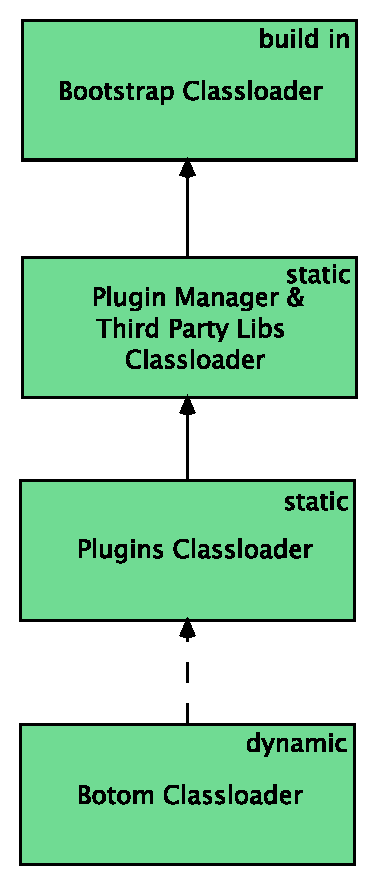
\includegraphics[width=0.3\textwidth]{material/images/Classloader-Hierarhie-Renew.pdf}
			\caption{\textsc{Renew} Klassenlader-System von Duvigneau \cite{Duvigneau09}}
			\label{fig:classLoadDuv}
		\end{figure}\bigbreak
		Duvigneaus Java Prototyp \cite{Duvigneau09} sollte eine Plugin-Verwaltung anbieten, die Plugins einfach sowie dynamisch neu konfigurieren lässt und das Hinzufügen und Entfernen von Plugins während der Laufzeit ermöglicht. Da der Prototyp nur die Praxistauglichkeit demonstrieren sollte, wurde eine \textit{schnelle} Variante implementiert, die nur die nötigste Funktionalität bereitstellt. Die Umsetzung der Klassenlader-Architektur aus der Abbildung \ref{fig:classLoadDuv} hat sich als ausreichend jedoch nicht Mängelfrei herausgestellt. Die Umsetzung unterstützte ein essenzielles Charakteristikum eines dynamischen Systems nicht, nämlich das Entladen der Plugin-Codebasis aus der Applikation während der Laufzeit. Denn die Plugins werden mit einem gemeinsamen Klassenlader in das System eingebunden, der keine Möglichkeit anbietet eine auserwählte Codebasis zu vergessen. Dementsprechend können Plugins, die mit einem gemeinsamen Klassenlader geladen worden sind, nicht mehr separat behandelt werden. Dies hat zur Folge, dass die Applikation während der Laufzeit ständig wächst und die Möglichkeit verliert Plugins zu aktualisieren. Somit ist man an einen Neustart angewiesen, der die initiale Codebasis zurücksetzt und die Plugins entfernt oder aktualisiert. Daraus folgt eine erhebliche Beeinträchtigung der Wartbarkeit und der Systemstabilität für Systeme mit einem permanenten Betrieb. \bigbreak
		Einer der möglichen Lösungsansätze beschreibt das Erstellen eines Klassenlader per Plugin und die Aufbereitung sowie Verwaltung der Kommunikation zwischen diesen. Da der mitgelieferte Klassenlader von Java nur einen übergeordnet Klassenlader akzeptiert, erfordert die Umsetzung eine eigene Klassenlader-Implementation, die variable Eltern-Kontenmenge akzeptiert und die Delegation intelligent umsetzt. Jedoch ist die genannte Umsetzung aufwändig und benötigt viel Eigenimplementation. \newline
		Eine Alternative bietet das \textit{OSGi} Rahmenwerk, welches auf dynamische Systeme ausgelegt ist und eine Komponentenbasierte Entwicklung ermöglicht. Das \textit{OSGi} Rahmenwerk organisiert den Code in \textit{bundles}, die sich auf separaten \textit{OSGi} Klassenlader-Implementation befinden und über eine Verknüpfung der \textit{bundles} eine Applikation modellieren. \newline
		Die Umsetzung von \textit{OSGi} im \textsc{Renew} Kontext hat sich für schwierig erwiesen, da die Verwaltung der Plugins als \textit{OSGi bundles} mit einem erweiterten Lebenszyklus und Kommunikationsschwierigkeiten den gewünschten Anforderungen nicht entsprach \cite{Duvigneau09}. Demzufolge wurde die Java-Umsetzung des Klassenlader-Systems \ref{fig:classLoadDuv} der \textit{OSGi}-Umsetzung vorgezogen und bis zum jetzigen Zeitpunkt einwandfrei betrieben. \bigbreak

		Mit der Einführung des Modulsystems von Java, ist Java fähig das genannt Problem anzugehen und bietet eine Alternative zu den beiden genannten Lösungsansätzen. Die Umsetzungsmöglichkeit der dynamischen Plugin-Verwaltung wird im nächsten Abschnitt der neu eingeführten Modulschichten diskutiert. 


\section{Durchführung} \label{sec:durchführung}
	Die wichtigen Szenarien für das Erreichen des gesetzten Ziels werden mit zwei Prototypen umgesetzt. Der \textsc{Renew} Prototyp wird eine kontinuierliche  Modularisierung der Plugins und dessen Betriebsfähigkeit mit nur zum Teil Modularisierter Codebasis abdecken. Dazu gehört das Erstellen einer neuen Projektstruktur für die auserwählten Plugins und behandelt auserwählte Richtlinien, die mit dem Modulsystem von Java eingeführt worden sind. Für das Anfertigen von ausführbar Code, wird das Gradle Werkzeug integriert, das einen Kompilation Kontext für die neuen Module erstellt. Dazu gehörten eine Abhängigkeitsverwaltung sowie Projektkopplung. Um die Plugins mit einender als Module zu verzahnen, werden Schnittellen untersucht und in der \textit{module-info} Konfigurationsdatei in den Plugins verankert. In der folgenden Evaluation wird das Ergebnis evaluiert und sauber aufbereitet.\bigbreak 

	Im Gegensatz dazu behandelt der \textsc{Mulan} Prototyp die Zusammenführung bestehender Systeme mit modularisiertem Code. Für die Umsetzung werden nur für das Spiel Settler relevanten \textsc{Mulan} Plugins erarbeitet und auf die minimale \textsc{Renew} Version aufgesetzt. Doch zuerst muss eine erweiterte Analyse der minimalen \textsc{Renew} Version durchgeführt werden, um die benötigten \textsc{Renew} Plugins für das \textsc{Mulan} Rahmenwerk nachzurüsten. Im weiteren Verlauf behandelt dieser Prototyp Konsequenzen der Umstellung auf eine neue \textsc{Renew} Grundlage und der benötigten Ausführungsschritte für die Adaption. Die Evaluation bewertet den Aufwand für die Umsetzung des Prototyps. 
\chapter{\textsc{Renew} Prototyp} 
	In diesem Kapitel entsteht ein Prototyp, der \textsc{Renew} schrittweise modularisiert, bis die Applikation den größten Teil ihre Funktionalität auf dem Modulpfad betreiben kann. \newline
	Für die Umsetzung des Prototyps werden zuerst Anforderungen erfasst, die der modularisierte \textsc{Renew} Prototyp erfüllen muss, um unserer Vision der Implementation zu entsprechen. Infolgedessen entsteht ein Implementierungsplan, sowie ein Prototyp.

\section{Anforderungen} \label{sec:anforderungen}
	Im Kern der Modernisierung von \textsc{Renew} liegt die Anpassung von \textsc{Renew} an das Modulsystem von Java und dessen Anforderungen an Applikationskomponenten. Aus den \textsc{Renew} Plugins sollen explizite Module entstehen, die auf dem Modulpfad betriebsfähig sein müssen. Die Drittanbieter-Bibliotheken sollen mit in den Modulpfad aufgenommen werden und als automatische Module ihre Aufgabe erfüllen. Zusätzlich darf die Migration und damit verbundene Anpassung und Aufbereitung der Mängel, die Kommunikation, sowie interne Funktionsweise von \textsc{Renew}, nicht verändern. Dementsprechend soll garantiert werden, dass die darunterliegende konzeptionelle Grundlage intakt bleibt.

% Was soll der Prototyp leisten 
\subsection{Interaktion}
	Der erste modulare \textsc{Renew} Prototyp soll mit einer minimalen Plugin Anzahl auf dem Modulpfad betriebsfähig sein, und eine Möglichkeit bieten, Petri-Netze zu erstellen, zu simulieren und zu serialisieren. Das heißt, es muss eine UI zu sehen sein, die mit den nötigen Werkzeugen und der darunterliegenden Logik, ausgestattet ist. 

\subsection{Projektstruktur}
	Für die Umsetzung des modularen \textsc{Renews}, wird für jedes Plugin eine moderne Projektstruktur benötigt, die den Inhalt entsprechend dem etablierten \textit{Maven} Standardverzeichnislayout, auf Java Module und die dafür benötigten Ressourcen, aufteilt. 

\subsection{Entwicklungsumgebung} 
	In der existierenden \textsc{Renew} Entwicklungsumgebung, werden alle Plugin Projekte durch eine versteckte \textit{.project} Datei, beschrieben. Das heißt, der Klassenpfad und die Bindung der Codebausteine geschehen versteckt und ist für den Entwickler, schwer zugänglich. Damit ist der Entwickler gezwungen, den weiten und verschachtelten Weg durch die UI Konfiguration von Eclipse zu betreten, der sich mit der Zeit verändern kann. Dieser Sachverhalt wurde von mir im letzten Projekt beobachtet und kostete Zeit für alle Projektteilnehmer, da die Universitätsrechner strikten Rechten unterliegen, die keine benutzerdefenierte Eclipse-Entwicklungsumgebung aufsetzen lässt. Darüber hinaus ist die Konfiguration von \textsc{Renew} in anderen Entwicklungsumgebungen wie IDEA oder Netbeans, mit der \textit{.project} Konfigurationsdatei nicht möglich. \bigbreak

	Um eine Entwicklungsumgebung unabhängige Konfiguration anzulegen, wird also ein neues Werkzeug benötigt. 

\subsection{Packaging}
	Da \textsc{Renew} an das Modulsystem angepasst werden muss, muss die Prozedur für das Kompilieren und das Verpacken der Codebasis, die Veränderung miterleben.\newline
	\textsc{Renew} benutzt zurzeit das \textit{Apache Ant}-Werkzeug, das alle Plugins kompiliert und in eine ausführbare Form bringt. Dieses ist in Jahre gekommen und enthält wesentlich geringeren Funktionsumfang gegenüber der aktuellen Konkurrenz, wie \textit{Maven} und \textit{Gradle}. Sie bieten eine Abhängigkeitsverwaltung, konfigurierbare Plugins und Programmiersprachen. Im Gesetz zu der aufgeblasenen XML-Konfiguration von Ant, die jeden kleinen Schritt ausführlich dokumentiert, beherrschen die modernen \textit{Build}-Werkzeuge, die Komplexität durch den \textit{Convention over Configuration} Ansatz und eine flexible Ausdrucksweise. \bigbreak

	Die minimale Version von \textsc{Renew} soll sich an einem modernen \textit{Build}-Werkzeug bedienen und ein ausführbares Ergebnis erzielen.

\section{Spezifikation}
	Um die Anforderungen umzusetzen, wird die erarbeitete minimale Version isoliert, umstrukturiert, und mit dem \textit{Gradle}-\textit{Build}-Werkzeug für das Arbeiten in der Entwicklungsumgebung \textit{IDEA}, aufgerüstet. Da \textit{Gradle} die Verwaltung des Projekts, sowie das Kompilieren und Erstellen von ausführbaren Paketen übernehmen kann, ist es für das Aufsetzen einer modernen und modularen Projektstruktur, eine gute Wahl.\newline
	Dafür muss das bestehende \textit{Ant-Build}-System analysiert und mit dem \textit{Gradle}-Werkzeug wiederaufgebaut werden. Dieses soll so gut wie möglich die bestehenden Drittanbieter-Bibliotheken verwalten, Module kompilieren und die benötigten Erweiterungen, wie das \textit{JavaCC}-Werkzeug, unterstützen.\bigbreak

	Nachdem die Projektstrukturen die passende Form angenommen haben, müssen die Projektabhängigkeiten analysiert und innerhalb der \textit{module-info.java} aufgenommen werden.\bigbreak

	Zuletzt entsteht eine bekannte Ordnerstruktur mit Drittanbieter-Bibliotheken, Plugins und Konfigurationsdateien, die unter zu Hilfenahme des \textit{Plugin Managers} verwaltet werden.

\section{Entwurf}
	Der Entwurf berücksichtigt die schrittweise Migration und lässt die \textsc{Renew} Applikation während der Gesamtmigration, betriebsfähig bleiben. Das heißt, Plugins auf den Klassenpfad, sowie Modulpfad, können nahtlos miteinander kommunizieren, und ihre Funktion während der Migration, weiterhin erfüllen.\bigbreak

	\begin{figure}[h!]
		\centering
		\begin{minipage}{7cm}
			\dirtree{%
			 .1 Project.
			 .2 src.
			 .3 main.
			 .4 java.
			 .5 de.application.purpose.
			 .6 de.
			 .7 application.
			 .8 purpose.
			 .4 resources.
			 }
		\end{minipage}
		\caption{Projektstruktur}
		\label{fig:projektstruktur}
	\end{figure}
	Für den ersten Prototypen wird zuerst eine Projektstruktur erstellt, die für jedes Plugin-Projekt die Möglichkeit bieten soll, aus mehreren Modulen zu bestehen. Dafür wird eine Struktur \ref{fig:projektstruktur} erstellt, die im Java Verzeichnis alle Module bündelt, die über den Modulnamen, disjunkt verwaltet werden. Nichtsdestotrotz gehören sie zum gleichen Projekt und teilen unter sich das Ressourcenverzeichnis, das im weiteren Verlauf, zum Erstellen der ausführbaren Pakete benötigt wird.\bigbreak
	       
	Nachdem die Projektstruktur der gewünschten Form entspricht, muss diese in der \textit{Gradle} Konfigurationsdatei verankert werden. Hierfür wird für jedes Projekt die Projektstruktur und dessen Abhängigkeiten in der \textit{build.gradle} Konfigurationsdateien \ref{fig:gradle_project} festgehalten, indem Java, sowie Ressourcen Stammverzeichnisse und Projekte definiert, und Drittanbieter-Bibliothekabhängigkeiten für den Kompilationspfad, bestimmt werden. \bigbreak

 		\begin{figure}[h!]
		\centering
		\begin{minipage}{7cm}
			\dirtree{%
			 .1 Project.
			 .2 build.gradle.
			 .2 settings.gradle.
			 .2 src.
			 .3 main.
			 .4 java.
			 .5 de.application.purpose.
			 .6 de.
			 .7 application.
			 .8 purpose.
			 .4 resources.
			 }
		\end{minipage}
		\caption{Gradle Konfiguration}
		\label{fig:gradle_project}
	\end{figure}
 	Die oben genannten Schritte müssen für jedes Projekt der minimalen Version von \textsc{Renew} durchgeführt und im Anschluss über die entsprechende Entwicklungsumgebung  validiert werden. Wenn die Entwicklungsumgebung alle Klassen und die benötigten Abhängigkeiten finden und kompilieren kann, wurden alle Projekte richtig deklariert, strukturiert und miteinander sauber verbunden. In diesem Zustand ist die komplette Struktur des Projekts innerhalb von \textit{Gradle} verpackt und kann von jeder Entwicklungsumgebung ausgelesen werden. \newline

	Da jetzt eine lauffähige minimale \textsc{Renew} Version für den Klassenpfad erstellt werden kann, ist es Zeit diese zu modularisieren und die einzelnen Plugins auf den Modulpfad zu migrieren. Dafür werde ich den \textit{bottom up} Ansatz aus dem Kapitel Migration \ref{sec:bottomUP} verwenden, und schrittweise die Plugins auf den Modulpfad bewegen.

	\begin{figure}[h!]
		\centering
		\begin{minipage}{7cm}
			\dirtree{%
			 .1 Project.
			 .2 build.gradle.
			 .2 settings.gradle.
			 .2 src.
			 .3 main.
			 .4 java.
			 .5 de.application.purpose.
			 .6 de.
			 .7 application.
			 .8 purpose.
			 .6 module-info.java.
			 .4 resources.
			 }
		\end{minipage}
		\caption{Modulumwandlung}
		\label{fig:module_project}
	\end{figure}

	Zuerst werden die Drittanbieter-Bibliotheken, wie \textit{log4j}, auf den Modulpfad als automatische Module eingebunden, und werden damit aus den Klassen- sowie Modulpfad, für die Nutzung, zugleich erreichbar sein. Anschließend werden Plugins als explizite Module migriert, die keine Plugin-Abhängigkeiten besitzen, und aus dem Modulpfad keine Zugriffe auf den Klassenpfad ausführen müssen. Beispielsweise besitzt das \textit{Util} Plugin keine Abhängigkeiten auf \textsc{Renew} Plugins und wird für die Ausführung auf dem Modulpfad, durch eine \textit{module-info.java} Konfigurationsdatei erweitert. Wie in der Abbildung \ref{fig:module_project} dargestellt, muss sich diese im Stammverzeichnis des Moduls befinden und die benötigten automatischen Module deklarieren.\newline
	Nachfolgend werden Plugins Schritt für Schritt auf den Modulpfad migriert, indem für jedes Plugin eine eigene \textit{module-info.java} Konfigurationsdateien angelegt wird, in der sich ihre Abhängigkeiten auf automatische Drittanbieter-Module, sowie explizite Plugin-Module, befinden.\bigbreak

	Dieses Vorgehen wird so lange durchgeführt, bis jedes Plugin sich auf dem Modulpfad befindet. 

\section{Umsetzung}

	Die Umsetzung realisiert den Entwurf und erstellt eine neue Projektstruktur für alle Plugins der minimalen \textsc{Renew} Version \ref{fig:plugin_deps}. Diese werden anschließend mit dem \textit{Gradle}-Werkzeug zusammengeführt und bilden ein kompilierfähiges Konstrukt. Danach werden die auserwählten Plugins, mit der \textit{module-info.java} versehen, und deklarieren innerhalb der Konfigurationsdateien, die zuvor vorgestellten Kommunikationskanäle \ref{sec:mod_kop} zwischen den Plugins.\newline
	Der Modularisierungsprozess geschieht iterativ und wird für jedes Plugin einzeln, nacheinander durchgeführt.
\newpage
\subsection{Umstrukturierung}

	Für die Umsetzung der Anforderungen und des Entwurfs, wird zuerst die Projektstruktur jedes Plugins angepasst. Dafür wird die Struktur jedes Plugins analysiert, umstrukturiert und im weiteren Verlauf, von Mängeln befreit. In den meisten Fällen, werden \textit{Split Packages} und gemischte Strukturen innerhalb der Codebasis erwartet.\bigbreak
	Zuerst wird eine grobe \textit{Maven} Projektstruktur erstellt, in der sich zusätzlich ein Plugin Wurzelverzeichnis befindet. Anschließend migriert man die Codebasis in das Plugin Wurzelverzeichnis, welches den neuen Plugin Namen trägt.

	\begin{figure}[h!]
		\centering
		\small
		\setlength{\DTbaselineskip}{7pt}
		\begin{minipage}{7cm}
			\dirtree{%
			 .1 Gui.
			 .2 build.xml.
			 .2 etc.
			 .3 README.gui.
			 .3 plugin.cfg.
			 .2 src.
			 .3 de.
			 .4 renew.
			 .5 ant.
			 .5 gui.
			 .6 images.
			 .6 menu.
			 .6 pnml.
			 .7 converter.
			 .7 creator.
			 .7 parser.
			 .4 io.
			 .5 exportFormats.
			 .5 importFormats. 
			 }
		\end{minipage}
		\caption{Gui Projekt}
		\label{fig:gui}
	\end{figure}

	Das Gui Plugin enthält die gängige mangelnde Organisation der Ressourcen. Zum Teil befinden sich diese im \textit{etc} Verzeichnis. Zum Teil sind diese in dem Java \textit{source set} Verzeichnis integriert, wie in der Abbildung \ref{fig:gui} dargestellt.\newline
	Um diese zu beheben, wird das Verzeichnis \textit{de.renew.gui.images}, das mit den \textit{png} und \textit{gif} Daten befüllt ist, in das Ressourcenverzeichnis migriert. Damit die Applikation diese wiederfindet, werden die Zugriffspfade für die Ressourcen innerhalb des Gui-Plugins, an das neue Verzeichnis angepasst, indem die internen statischen Konstanten, wie \textit{CPNIMAGES}, auf den entsprechenden Ort verweisen. \newline
	Zum Schluss werden die \textit{README} und die \textit{plugin.cfg}  aus dem \textit{etc} Verzeichnis in das Ressourcenverzeichnis bewegt. Somit ist eine Struktur erstellt worden, die sich auf das Modulsystem von Java anwenden lässt. \bigbreak

	\begin{figure}[h!]
		\centering
		\small
		\setlength{\DTbaselineskip}{7pt}
		\begin{minipage}{7cm}
			\dirtree{%
			 .1 Formalism.
			 .2 build.xml.
			 .2 etc.
			 .3 README.formalism.
			 .3 plugin.cfg.
			 .2 src.
			 .3 de.
			 .4 renew.
			 .5 formalism.
			 .6 base.
			 .6 bool.
			 .6 function.
			 .7 java.
			 .8 JavaNetParser.jj.
			 .7 pt.
			 }
		\end{minipage}
	  \caption{Formalism Projekt}
	  \label{fig:formalism}
	\end{figure}

	Andere Plugins wie \textit{Formalism}, \textit{CH} oder \textit{Misc}, besitzen \textit{JavaCC} Dateien. Wie im Beispiel \ref{fig:formalism} dargestellt. Diese enden auf \textit{jj}. Letzt genannte erstellen Java Netz Grammatiken und wandeln die Java-Basis für die Ausführung ab. Sie liegen lose zwischen den Java Klassen und werden von den Java Compiler nicht interpretiert. Daher ist es sinnvoll, diese in ein eigenes \textit{SourceSet} auszulagern, und für den \textit{JavaCC}-Compiler für die Übersetzung, zu gruppieren.

	\begin{figure}[h!]
		\centering
		\footnotesize
		\setlength{\DTbaselineskip}{10pt}
		\begin{minipage}{.45\textwidth}
			\dirtree{%
			 .1 Formalism.
			 .2 src.
			 .3 main.
			 .4 java.
			 .5 de.renew.formalism.
			 .6 de.
			 .7 renew.
			 .8 formalism.
			 .9 base.
			 .9 bool.
			 .9 function.
			 .9 java.
			 .9 pt.
			 .4 javacc.
			 .5 JavaNetParser.jj.
			 .4 resources.
			 .5 README.formalism.
			 .5 plugin.cfg.
			 }
		\end{minipage}
		\begin{minipage}{.5\textwidth}
			\dirtree{%
			 .1 Gui.
			 .2 src.
			 .3 main.
			 .4 java.
			 .5 de.renew.gui.
			 .6 de.
			 .7 renew.
			 .8 gui.
			 .9 menu.
			 .9 pnml.
			 .10 conv.rng.
			 .10 converter.
			 .10 creator.
			 .10 parser.
			 .10 ptNetb.pntd.
			 .10 refNetb.pntd.
			 .9 io.
			 .10 exportFormats.
			 .10 importFormats.
			 .9 tasks.
			 .5 resources.
			 .6 README.gui.
			 .5 images.
			 .5 plugin.cfg.
			 }
		\end{minipage}
	  \caption{Resultierende Projektstrukturen}
	  \label{fig:resultStr}
	\end{figure}

	Das finale Resultat in der Abbildung \ref{fig:resultStr} erlaubt, eine einfache Paketstruktur-Analyse durchzuführen, um die \textit{Split Packages} zu identifizieren. \bigbreak

	Auf den ersten Blick kann eine Überschneidung zwischen den Gui und den RenewAnt Plugin erkannt werden, da beide den \textit{de.renew.ant} Namensraum besetzen, der sich um bestimmte \textit{Ant} spezifische Aufgaben kümmert. Aufgrund dessen, wird der Namensraum in dem Gui Plugin in \textit{task} zu Gunsten des RenewAnt Plugins umbenannt. Des Weiteren könnten beide \textit{Task's} in den RenewAnt Plugin verschoben werden, da dieser keine Abhängigkeiten in dem Gui Plugin besitzt, und nicht in den Aufgabenbereich der UI fällt. 

\subsection{Gradle}

 	Um die Zyklen zu erkennen, wird ein \textit{Gradle-Build}-Skript erstellt, der die Java \textit{SourceSets} für den Kompilationsschritt definiert und die benötigten Projekte, sowie Drittanbieter-Bibliotheken, auf den Projektklassenpfad einbindet. Mit der Unterstützung der \textit{Gradle}-Projektumgebung und einer \textit{IDE}, können anschließend alle Abhängigkeiten aufgedeckt, und auf Zyklen überprüft werden. \newline
 	Für die Umsetzung der \textit{Gradle}-Projektumgebung wird zuerst das bestehende \textit{Ant}-System analysiert. Dieses besteht aus Skripten, die sich in jedem Plugin befinden und für die entsprechenden Projekte ausführbare Jar's erstellen. Die \textit{Ant}-Skripte sind sehr ähnlich aufgebaut und wiederholen ein Erstellungsmuster für alle Plugins. \newline
	\begin{figure}[h!]
	  \centering
	  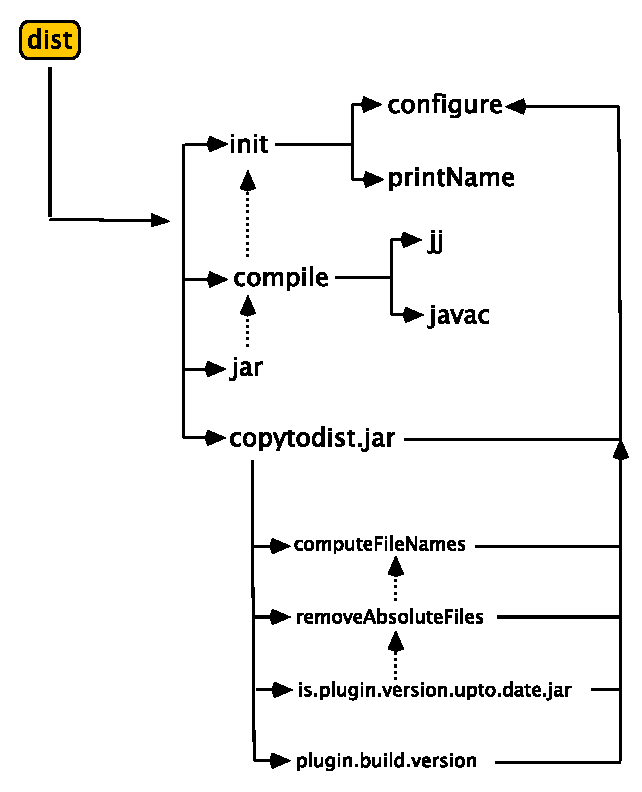
\includegraphics[width=0.5\textwidth]{material/images/ant-build.pdf}
	  \caption{Ant Skript}
	  \label{fig:antscript}
	\end{figure}

	In der Abbildung \ref{fig:antscript} ist ein Modell für die Erstellung eines Plugins mit dem \textit{Ant}-Werkzeug, dargestellt. \textit{Ant} initiiert das Skript mit Feldern und benötigten Variablen aus einer globalen Konfiguration, generiert Java Daten mit dem \textit{jj Target}, kompiliert und verpackt die ausführbaren Klassen. \bigbreak
	
	Für die \textit{Gradle}-Umsetzung werden Schritte, die über die etablierten Operationen zum Erstellen einer ausführbaren Java Applikation wahrgenommen, und in die folgende \textit{Gradle}-Umgebung eingebunden.\newline
	Dafür wird zuerst ein übergeordneter \textit{Gradle}-Projekt deklariert, das Subprojekte aus allen Plugin Verzeichnissen erstellt.\bigbreak

	\begin{figure}[h!]
	  \centering
	  \includegraphics[width=0.6\textwidth]{material/images/settingsgradle.pdf}
	  \caption{Subprojekte}
	  \label{fig:subprojekte}
	\end{figure}

 	Die \textit{settings.gradle} Datei in der Abbildung \ref{fig:subprojekte}, die in der Konfigurationsphase des \textit{Gradle}-Lebenszyklus ausgelesen wird, ist für diesen Konfigurationsschritt zuständig und kann mithilfe von \textit{Groovy}, beliebigen Code für die Deklaration der Projekte enthalten. In diesem Fall werden alle Verzeichnisse, die mit einem Großbuchstaben anfangen, als \textit{Gradle}-Subprojekte eingebunden.\bigbreak

	\begin{figure}[h!]
	  \centering
	  \includegraphics[width=0.7\textwidth]{material/images/sourcesets.pdf}
	  \caption{SourceSets}
	  \label{fig:Source_Sets}
	\end{figure}

 	Anschließend müssen die Java \textit{SourceSets} des Projekts bestimmt werden. Um die Umsetzung so einfach wie möglich zu gestalten, wird in der \textit{build.gradle} Konfigurationsdatei, die für die Ausführungsphase zuständig ist, eine \textit{subprojects} Konfiguration angelegt, die für jedes Subprojekt die interne Projektstruktur definieren lässt. Diese beschreibt den Ort, an dem sich  Verzeichnisse mit den Java Code und den dazugehörigen Ressourcen, befinden sollen.\bigbreak

	\begin{figure}[h!]
	  \centering
	  \includegraphics[width=0.6\textwidth]{material/images/gradle/dependencies.pdf}
	  \caption{Drittanbieter-Bibliotheken}
	  \label{fig:deps}
	\end{figure}

 	Im nächsten Schritt werden global genutzte Drittanbieter-Bibliotheken deklariert. Diese werden aus dem \textit{Maven Repository} beim Initiieren des Projekts geladen und auf den Klassenpfad aller Plugin Projekte eingebunden. Somit liegt die Verwaltung der Bibliotheken und der dazugehörigen Version an den \textit{Maven Repository}, und muss nicht mehr im \textit{GitLab Repository} bereitgestellt werden.\newline
 	Zusätzlich erleichtert die Deklaration der Drittanbieter-Bibliotheken, unter einer separaten Konfiguration, die Aufgabe der manuellen Erstellung der Klassenpfade, und die Einbindung der Bibliotheken in der Entwicklungsumgebung. Dabei wird die Konfiguration von der Entwicklungsumgebung automatisch aufgegriffen und auf das Projekt angewandt.\bigbreak

	\begin{figure}[h!]
	  \centering
	  \includegraphics[width=0.6\textwidth]{material/images/gradle/configurations.pdf}
	  \caption{Klassenpfade}
	  \label{fig:kPath}
	\end{figure}

 	Um die Klassenpfade voneinander zu trennen, werden zusätzliche Konfigurationen mit dem Namen \textit{plugin} und \textit{automatic} eingeführt, die Plugin Code und Drittanbieter-Bibliotheken voneinander trennen und für das Kompilieren, zusammenführen. Somit können diese getrennt voneinander verwaltet, modifiziert und bei Bedarf, an bestimmte Aufgaben angepasst werden.\bigbreak

	\begin{figure}[h!]
	  \centering
	  \includegraphics[width=\textwidth]{material/images/jar.pdf}
	  \caption{Jar Task}
	  \label{fig:jar}
	\end{figure}

	Zum Schluss der globalen Konfiguration, wird ein \textit{jar} Task angelegt, der für ein gegebenes \textit{SourceSet} ein \textit{jar}-Archiv für jedes Plugin mit den dazugehörigen Ressourcen erstellt.\newline
	Damit ist die globale Konfiguration der \textsc{Renew} Plugins beendet und bereit für die individuelle Anpassung der Plugin Bedürfnisse.\bigbreak

	\begin{figure}[h!]
	  \centering
	  \includegraphics[width=0.8\textwidth]{material/images/gradle/winmangradle.pdf}
	  \caption{Individuelle Konfiguration}
	  \label{fig:windmang}
	\end{figure}

	Jedes einzelne Plugin benötigt neben einem internen Namen, der dazugehörigen Drittanbieter-Bibliotheken, auch Plugin-Abhängigkeiten. Dafür wird in der Plugin \textit{build.gradle} Konfigurationsdatei, der Name unter den \textit{extension properties} deklariert und die bereits geerbten Abhängigkeiten erweitert. In der Abbildung \ref{fig:windmang} wird das WindowManagement Plugin durch mehrere lokale, modifizierte Drittanbieter-Bibliotheken und durch das Plugin Projekt erweitert, um alle Benötigen Abhängigkeiten abzudecken.\bigbreak

	Ant spielt eine unerwartet wichtige Rolle für das Erstellen der \textsc{Renew} Plugins. Denn \textit{Ant} verwaltet nicht nur das Kompilieren und Erstellen von ausführbaren Archiven, sondern ist auch zuständig für die Verwaltung der zusätzlichen Ausführungsschritte, die \textsc{Renew} Code sowie Ressourcen generieren. Zum Teil sind es Drittanbieter-Werkzeuge, wie der \textit{JavaCC}-Compiler, als auch speziell für \textsc{Renew} entwickelte Verfahren. \bigbreak

	\begin{figure}[h!]
	  \centering
	  \includegraphics[width=\textwidth]{material/images/gradle/javacc.pdf}
	  \caption{Java Compiler Compiler}
	  \label{fig:javacc}
	\end{figure}

	Für die Konfiguration der auserwählten Plugins, spielt der \textit{JavaCC}-Parser eine große Rolle, denn dieser wandelt eine Grammatikspezifikation in ausführbaren Java Code um. Die genannte Technik wird in dem \textit{Formalism}, \textit{Feature Structures}, \textit{CH} und in dem \textit{Misc}-Plugin verwendet. Der \textit{JavaCC} Parser erstellt Java Klassen, die obligatorisch für die Ausführung von \textsc{Renew} präsent sein müssen. Dementsprechend werden diese als generierte Ressourcen im \textit{build} Verzeichnis abgelegt und dem Java \textit{SourceSet} beigefügt. \bigbreak

	Andere Plugins benötigen keine Drittanbieter Software, sondern beruhen auf eigenen Verfahren, die ausführbaren Code und Artefakte für die Plugins herstellen. Für die Umsetzung der Ausführungsschritte, wurden an \textit{Ant} angepasste Java Klassen geschrieben, die auf der \textsc{Renew}-Logik beruhen. Diese können von \textit{Ant} aufgerufen und durchgeführt werden können. Infolgedessen stellt sich die Frage, wie die Ausführungsschritte aus der \textit{Ant}- in die \textit{Gradle}-Umgebung migriert werden könne. \newline
	Um die Anwender von \textit{Ant} und \textit{Maven} von \textit{Gradle} zu überzeugen, integriert \textit{Gradle} beide Systeme und lässt deren Funktionalität benutzen und steuern. Somit ist ein nahtloser Übergang auf \textit{Gradle} garantiert und überzeugt die Anwender durch die mitgelieferte Flexibilität.\bigbreak
	
	Um die erstellten \textsc{Renew} Verfahren in \textit{Gradle} zu übernehmen, kann auf eine mitgelieferte \textit{Ant}-Instanz aus \textit{Gradle} zugegriffen und für die Konfiguration der Verfahren aufbereitet werden. Anschließend kann über die \textit{Ant}-Instanz die konfigurierte Logik aufgerufen und ausgeführt werden. Obwohl das Konstrukt beherrschbar erscheint, erfordert dies trotz Allem eine gute Kenntnis der \textit{Ant}-Funktionalität. Und kann bei unerfahrenen Entwicklern zu irreführenden Annahmen führen.
	\begin{figure}[h!]
		\centering
		\includegraphics[width=\textwidth]{material/images/gradle/antTasks.pdf}
		\caption{Java Compiler Compiler}
		\label{fig:javaccAnt}
  	\end{figure}


	Jedes einzelne Plugin wird auf diese Weise konfiguriert und enthält einen Namen, sowie zusätzliche Abhängigkeiten. Hiermit ist die Vorbereitung für die Modularisierung abgeschlossen.


\subsection{Modularisierung}	
	Nachdem alle benötigen \textsc{Renew} Plugins kompiliert, verpackt und ausgeführt werden können, müssen die neu entstandenen Abhängigkeitsbeziehungen analysiert werden. Die Analyse der Plugins geschieht nun über die erstellten \textit{Gradle}-Scripte, die für jedes Projekt die benötigten Bibliotheken und ebenso die benötigten Projekt für die Kompilation, deklarieren. Aus den angeforderten Bibliotheken und Projekten, wird ein Graph erstellt, der Zyklen und versteckte Abhängigkeiten, offenlegt. \bigbreak

	\begin{figure}[h!]
	  \centering
	  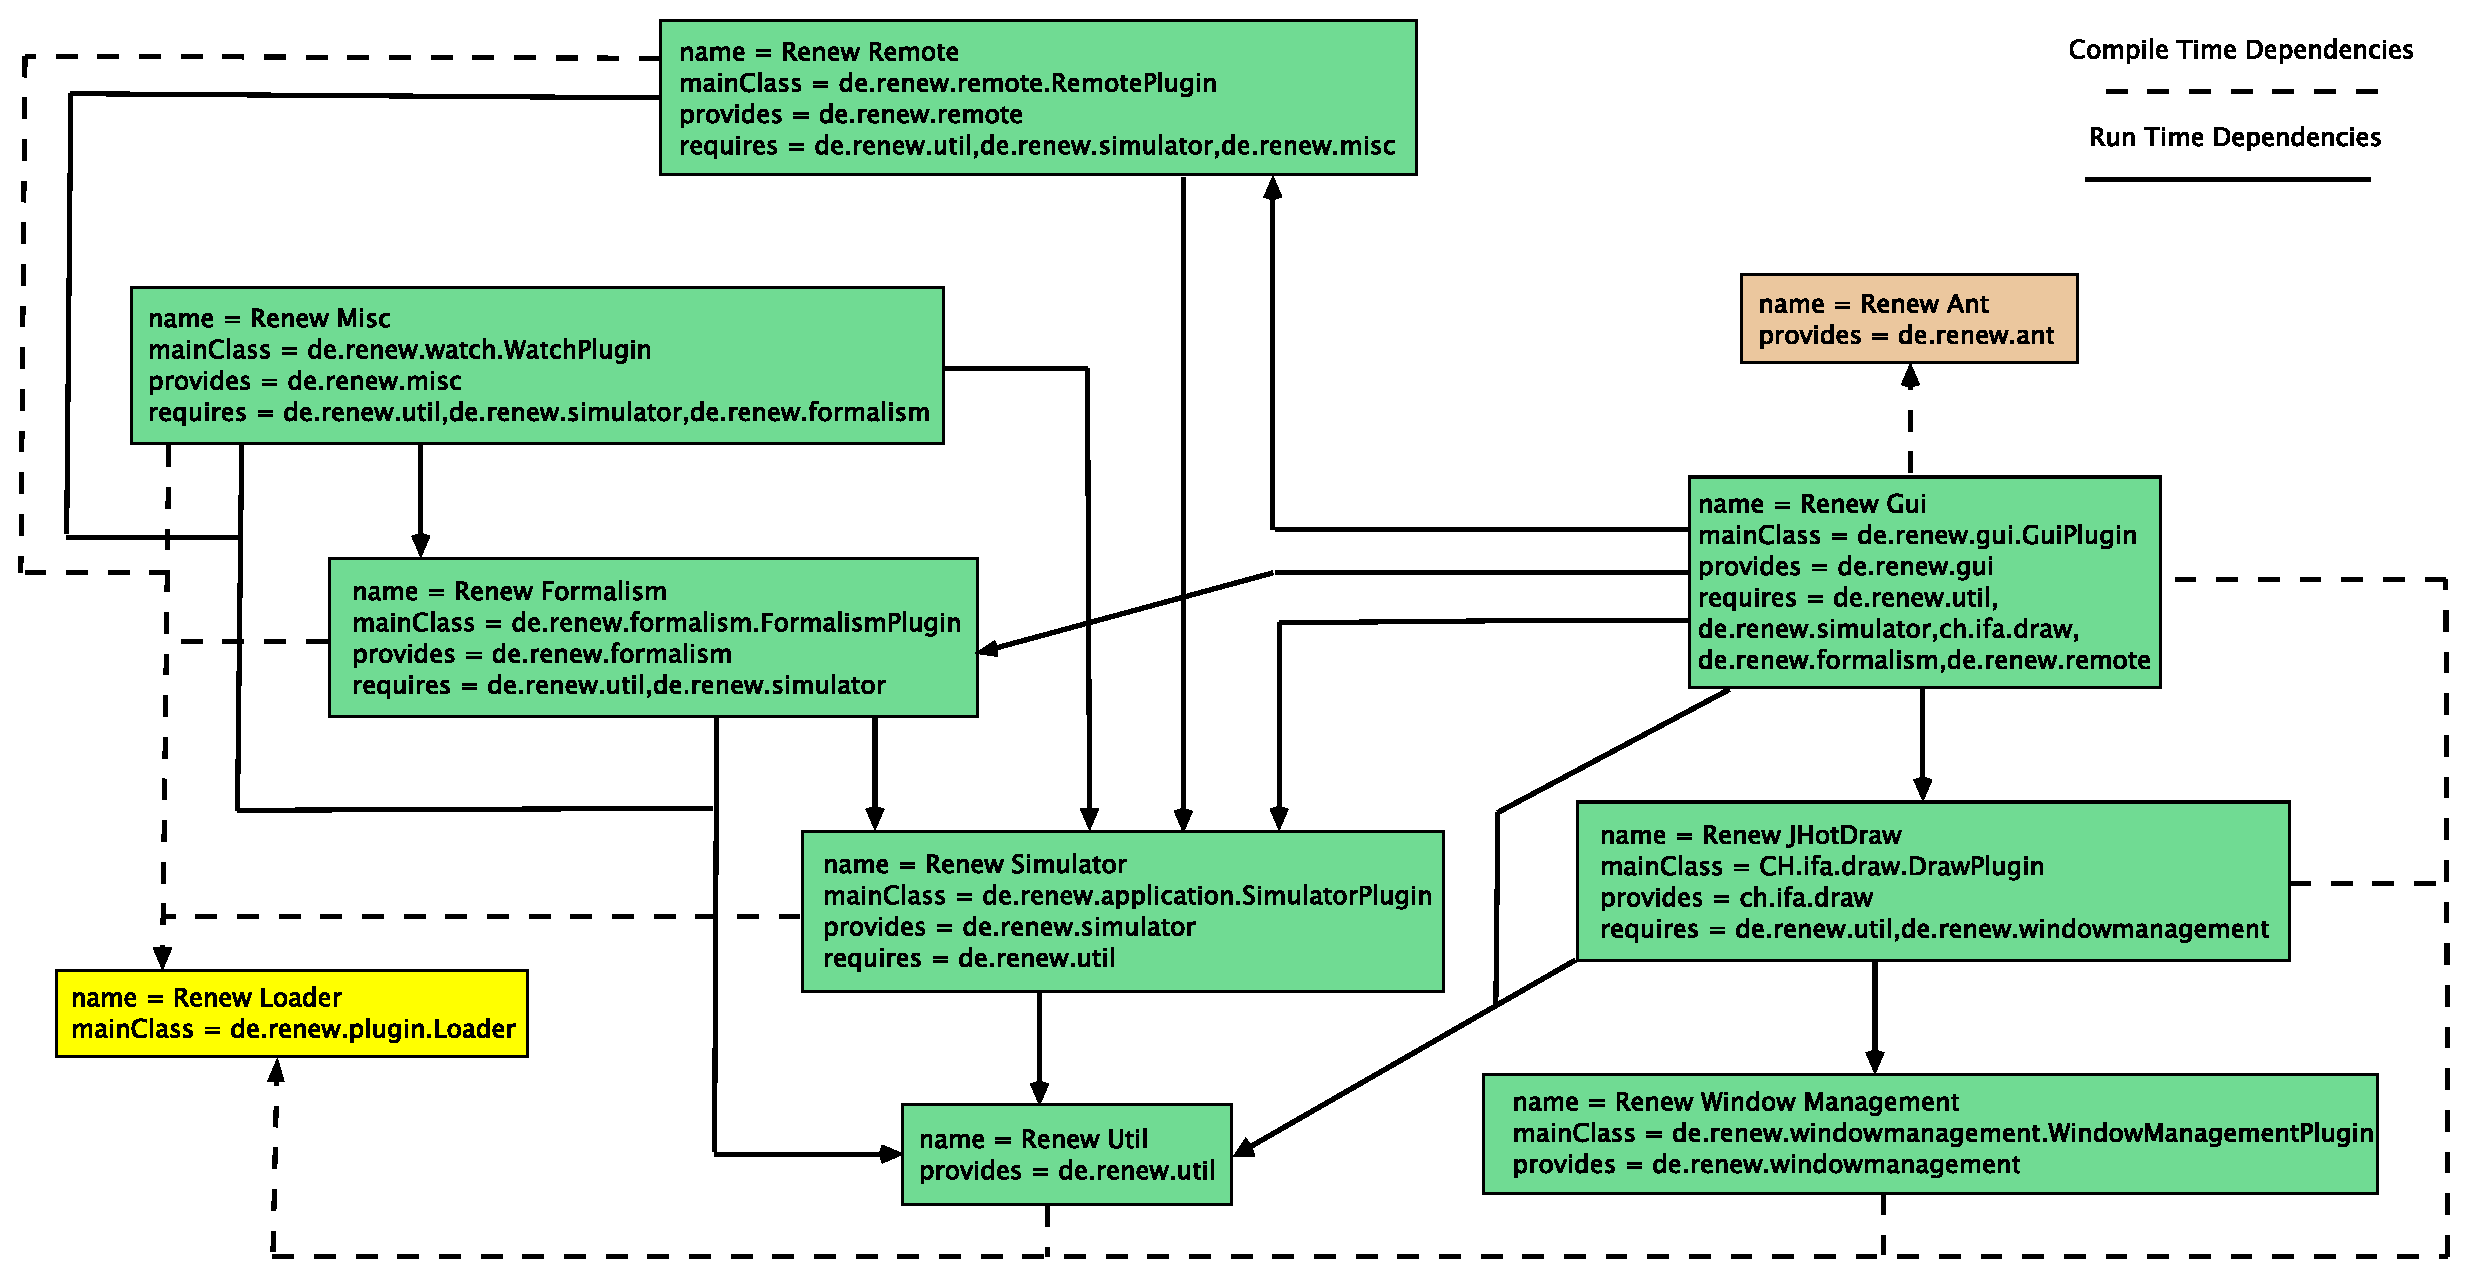
\includegraphics[scale=0.45, angle=90]{material/images/renew_plugin_dependencies-module-info.pdf}
	  \caption{Kompilation Abhängigkeiten}
	  \label{fig:mod_deps}
	\end{figure}

	Der neu entstandene Graph wurde im Vergleich zum Graphen aus der Ausgangssituation (s.\ref{fig:plugin_deps}), durch ein Plugin erweitert und bindet alle Plugins an das \textit{Loader}-Projekt. Des Weiteren sind keine weiteren Zyklen zu beobachten (s. Abbildung \ref{fig:mod_deps}) und dementsprechend, müssen auch keine weiteren Anpassungen durchgeführt werden. \bigbreak

	Die Migration von der minimalen Version von \textsc{Renew} wird von den \textit{Loader, Util} und \textit{WindowManagement} Plugin eingeleitet. Diese besitzen keine Abhängigkeiten innerhalb der Plugin-Menge und brauchen  aus dem Modulpfad keinen Zugriff auf den Klassenpfad, nachdem sie sich auf dem Modulpfad befinden. Im Gegensatz dazu, behalten Plugins, die sich auf dem Klassenpfad befinden und als ein unbenanntes Modul interpretiert werden, alle Zugriffsrechte auf die interne Struktur migrierter Plugins. Dies wurde bereits im Abschnitt \ref{fig:modacc} beschrieben.\bigbreak

	Da ein Modul seine eigenen Abhängigkeiten verwalten muss, wird für jedes Plugin eine \textit{module-info.java} Konfigurationsdatei angelegt, die Java internen, sowie Drittanbieter-Bibliotheken auflistet. Für die ersten Module werden die erforderlichen Bibliotheken inklusive des \textit{Loader}-Plugins in der Konfigurationsdatei mit dem Schlüssel \textit{requires} verankert. Zusätzlich werden die  dazugehörigen Drittanbieter-Bibliotheken aus dem Klassenpfad, auf dem Modulpfad als automatische Module, aufgesetzt.

	\begin{figure}[h!]
	  \centering
	  \includegraphics[width=0.7\textwidth]{material/images/loaderUtil-info.png}
	  \caption{Benötigten Bibliotheken}
	  \label{fig:loaderUtil}
	\end{figure}

	In diesem Zustand wird \textsc{Renew} kompiliert und ausgeführt. Das Ergebnis ist eine lauffähige Applikation, die ihre vollständige Funktion zugleich aus dem Modul- und Klassenpfad bezieht und identisch zu der initialen minimalen Version von \textsc{Renew} funktioniert.\newline
	Im nächsten Schritt werden Plugins migriert, die nur auf die neu entstandenen Module aufsetzen, wie zum Beispiel das \textit{Simulator} und das \textit{JHotDraw} Plugin. Ihre Abhängigkeiten liegen auf dem Modulpfad Daher gibt es keinen Grund, mit dem Klassenpfad zu interagieren. \newline
	Da diese die zweite Modulschicht repräsentieren, fordern sie bestimmte Funktionalität mit dem \textit{requires} Schlüssel aus den \textit{Loader, Util} und \textit{WindowManagement} Plugins. Um dieser Anforderung zu entsprechen, müssen die notwendigen Plugins ihre Pakete  explizit für ihre Nutzer öffnen. Dazu deklarieren die angeforderten Plugins in ihrer \textit{module-info.java} mit dem \textit{exports} Schlüssel Pakete, die sie für andere Plugins zur Verfügung stellen möchten.

	\begin{figure}[h!]
	  \centering
	  \includegraphics[width=0.7\textwidth]{material/images/utilCH-info.png}
	  \caption{Exportierte Pakete}
	  \label{fig:utilCH}
	\end{figure}

	In der Abbildung \ref{fig:utilCH} wurde das \textit{Util}-Plugin-Modul angepasst und bietet jetzt für den Gebrauch, das \textit{de.renew.util} Paket an.\newline
	Die Adaption der bestehenden Module muss mit jedem neuem Modul an die angeforderten Pakete und Klassen angepasst werden, bis alle Abhängigkeiten erfüllt sind.\newline
	Damit sind die notwendigen Schritte für die Modularisierung bestimmt worden und können, bis sich alle Plugins auf dem Modulpfad befinden, in einem Zyklus durchgeführt werden. Dies geschieht durch das Auslesen und Definieren der Plugin Kompilation- sowie Laufzeit-Abhängigkeiten aus dem \textit{Gradle-Build}-Skript, mit dem Schlüssel \textit{requires}, und das Nachrüsten der Schnittstellen bestehender Module mit dem \textit{exports} Schlüssel. \bigbreak

	In der folgenden Abbildung wird die komplette Migration in vier Schritten dargestellt. Zuerst wird das \textit{Loader}, das \textit{Utils} und das \textit{Window Management} Plugin migriert, da diese laut der Ausgangssituation keine Abhängigkeiten im Klassenpfad besitzen und nicht aus dem Modulpfad auf den Klassenpfad zugreifen müssen. Im nächsten Schritt werden Plugins modularisiert, die nur auf den Modulpfad angewiesen sind. Das wäre der \textit{Simulator}- und der \textit{JHotDraw}-Plugin. Da alle Abhängigkeiten des Plugin \textit{Remote} und \textit{Formalism} auf dem Modulpfad bewegt worden sind, können diese der Modulmenge beigefügt werden. Zum Schluss bleiben Plugins, mit weit gefächerten Plugin-Abhängigkeiten, wie zum Beispiel das \textit{Misc} oder das \textit{Gui} Plugin.  \bigbreak

	\begin{figure}[hbt!] 
	  \centering
	  \includegraphics[width=0.997\textwidth]{material/images/renew_plugin_dependencies-migrate_1b.pdf}\bigbreak\bigbreak
	  \includegraphics[width=0.997\textwidth]{material/images/renew_plugin_dependencies-migrate_2b.pdf}\bigbreak\bigbreak
  	  \includegraphics[width=0.997\textwidth]{material/images/renew_plugin_dependencies-migrate_3b.pdf}\bigbreak\bigbreak
  	\end{figure}
  	\begin{figure}[t!] 
	  \centering
  	  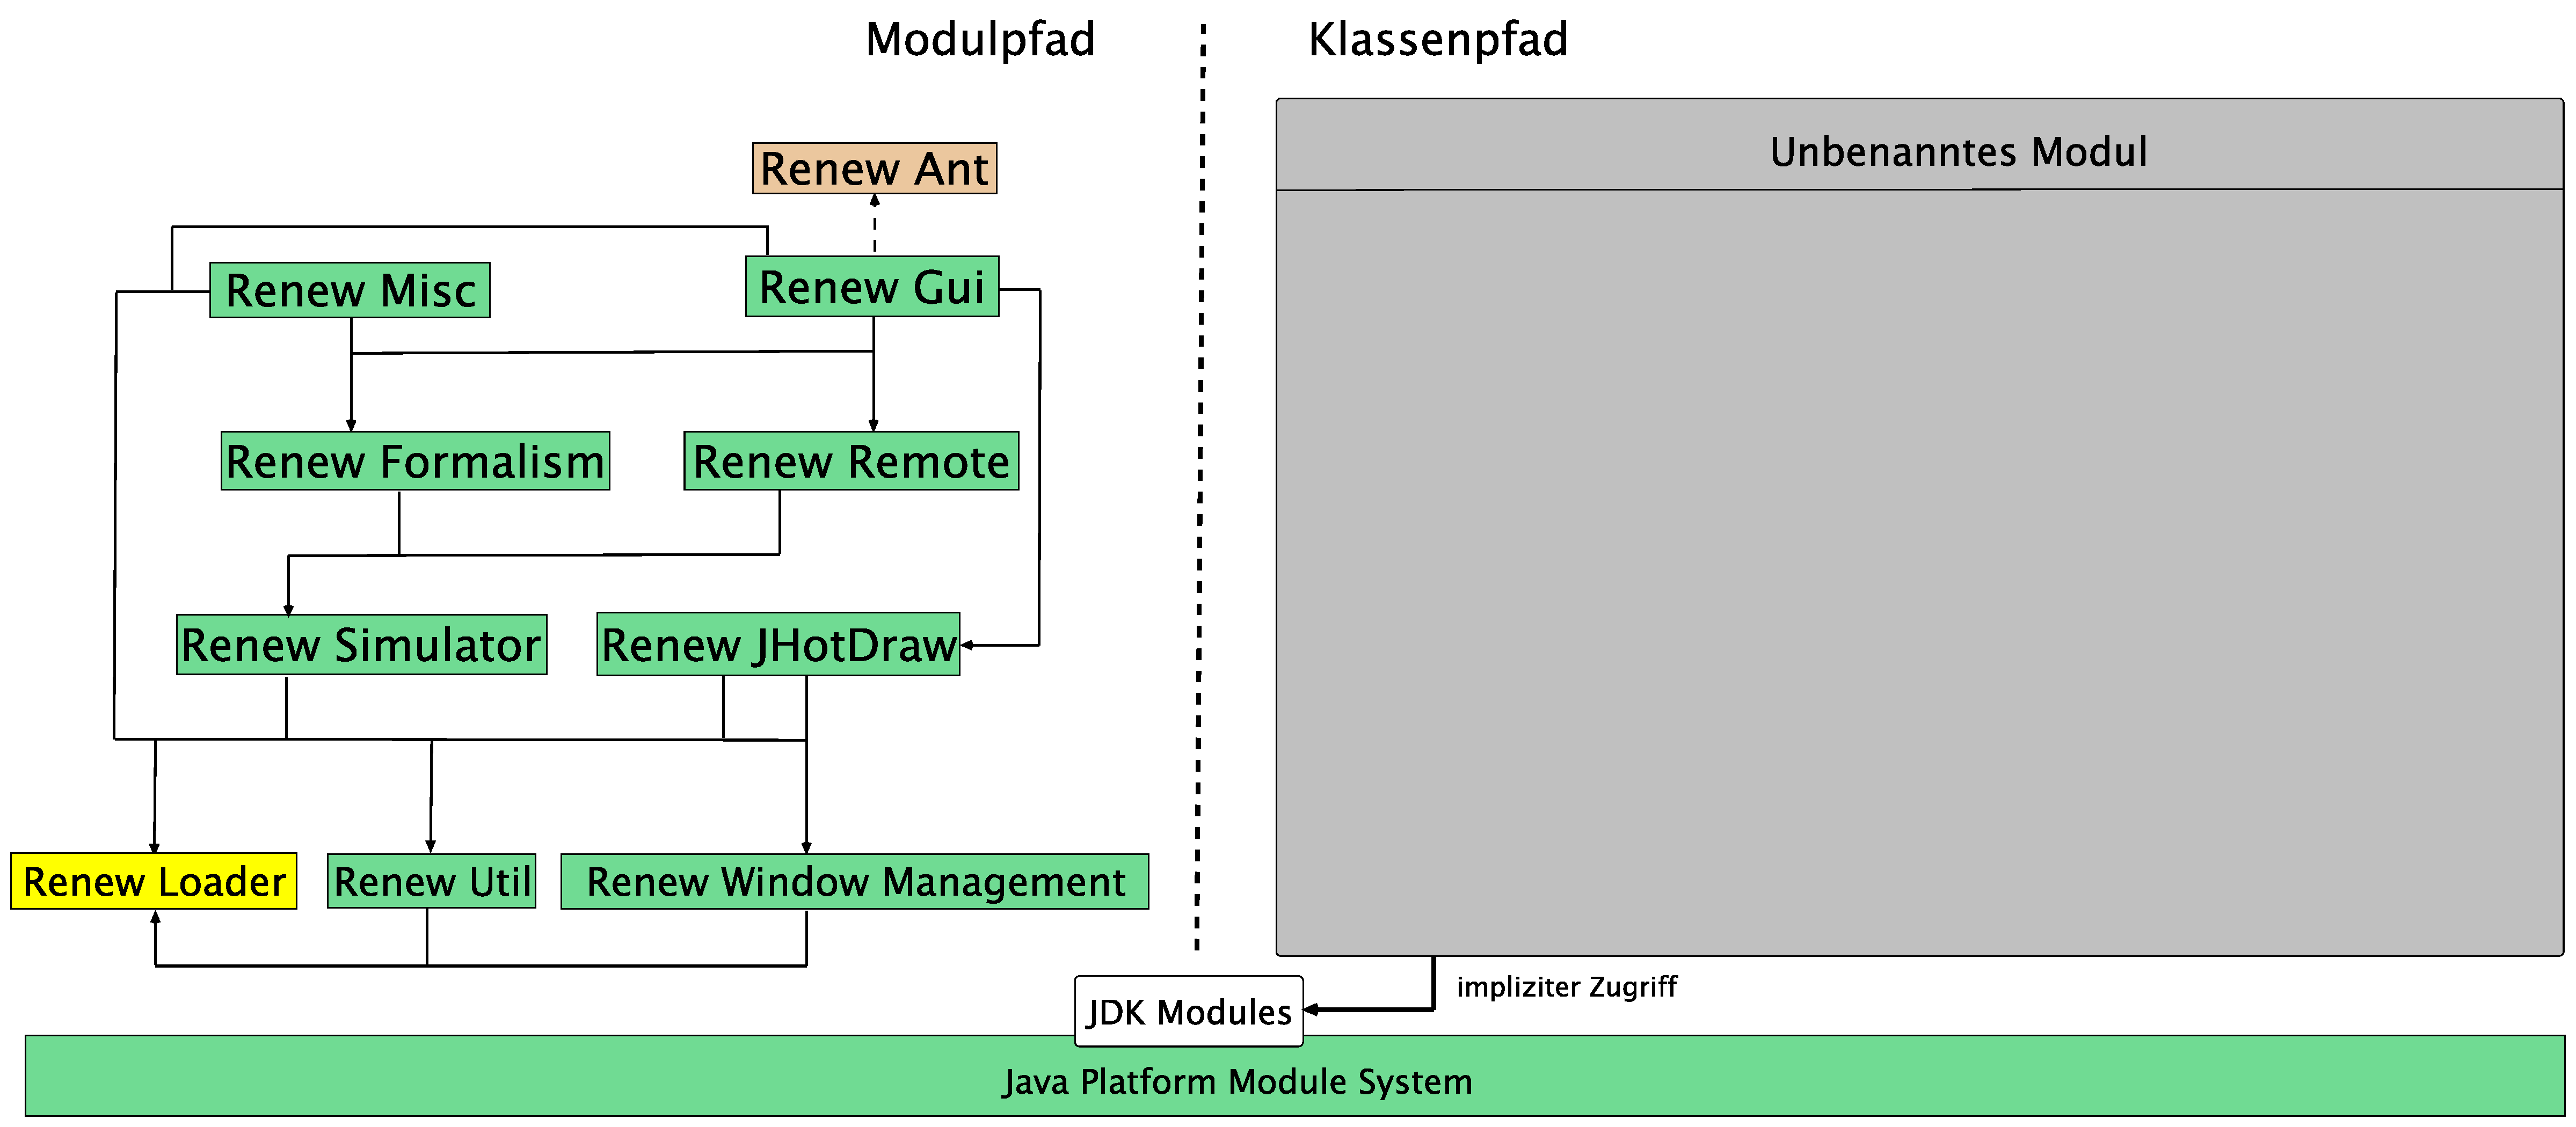
\includegraphics[width=0.997\textwidth]{material/images/renew_plugin_dependencies-migrate_4b.pdf}
  	  \caption{Migration}
	  \label{fig:mig}
	\end{figure}

\newpage  
\phantom{This text will be invisible}
\newpage
\section{Evaluation}
	Die Evaluation des ersten Prototyps bewertet das Ergebnis des gesetzten Ziels, nämlich die Erstellung einer minimalen \textsc{Renew} Version für das Modulsystem von Java. Dafür werden die Schlüsselaktionen der Migration, wie Projektstruktur, Projektverwaltung und die Modulumsetzung, nacheinander kritisch beleuchtet.

\subsection{Struktur} \label{sub:struktur}
	Die Anforderung eine minimale Version von \textsc{Renew} zu modularisieren und mit einem modernen Werkzeug zu verwalten wurde erfüllt. Diese Aufgabe beinhaltete das Umstrukturieren der Plugin-Codebasis, die es erlaubt, zusätzliche Module innerhalb eines Plugins anzulegen. Jedoch gab es unerwartete Strukturänderungen, die durchgeführt werden mussten. Zum Beispiel besitzen einige Plugins, wie das \textit{Util, Loader} und \textit{Simulator}-Plugin Test-Klassen, die in die neue Struktur eingebunden werden müssten. Demzufolge musste laut dem \textit{Maven} Standard-Layout, ein \textit{src/test/java/module.name} Test-Ressourcenverzeichnis, mit den dazugehörigen Test Klassen, angelegt und verwaltet werden. \newline

	Des Weiteren werden JavaCC Klassen separat von den Java Ressourcen untergebracht und von einem \textit{Gradle} Plugin ausgeführt. Dies hat zur Folge, dass der generierte Code umgeleitet werden muss, um an der entsprechenden Position seine Funktion erfüllen zu können. Zusätzlich muss der \textit{JavaCC}-Compiler den Java Code generieren, bevor der Java Compiler mit der Übersetzung beginnt, denn die generierten Java Klassen bilden die Basis für die Plugins. Somit sind sie für die Kompilation zwingend erforderlich. Diesbezüglich wurde der \textit{Gradle Task Graph} modifiziert, um die entsprechende Reihenfolge der Ausführung zu erfüllen. Daraus ergibt sich eine Komplexität, die für \textsc{Renew} neu ist und in der Zukunft sorgfältig gewartet werden muss. \bigbreak

\subsection{Verwaltung} \label{sub:verwaltung}
	Ein wesentlicher Vorteil der modernen \textit{Build} Tools wie \textit{Gradle} und \textit{Maven}, ist die Verwaltung der verwendeten Drittanbieter-Bibliotheken. Diese laden und binden benötigte Bibliotheken mit dem kompletten Abhängigkeitsgraphen in das Projekt ein, ohne die zwingende Einarbeitung in die Struktur der genutzten Bibliothek durch den Entwickler. Somit wird viel Zeit gespart, da man sich mit dem Kontext und den darunterliegenden Bausteinen, wie zum Beispiel \textit{Core}, \textit{Common} und \textit{Util}, nicht beschäftigen muss. \newline

	Die Verwaltung der Bibliotheken spielt eine große Rolle für \textsc{Renew}, da im Verlauf der Entwicklung, Drittanbieter-Bibliotheken angepasst wurden und somit keine Möglichkeit mehr besteht, eine saubere Version der Bibliothek einzubinden. Infolgedessen entstehen unsaubere Abhängigkeiten, die nicht aktualisiert werden können. Diese werden wie zuvor, durch das Auslesen aus einem lokalen \textit{libs} Verzeichnis, in das Projekt eingebunden und müssen in der Zukunft, für eine saubere Umsetzung, der benutzerdefinierten Logik, befreit werden.\bigbreak

	Ein zusätzlicher Vorteil der neuen Projektverwaltung liegt in der neuen Umsetzung mit einer Programmiersprache, die es erlaubt, mit Feldern, Variablen, Schleifen und Objekten zu arbeiten. Dies hat zur Folge, dass der Übergang von den \textsc{Renew} Java-Code, zu den \textit{Build}-Skript von \textit{Gradle}, für den Entwickler leichter nachzuvollziehen ist, und somit Akzeptanz und Anpassungsfähigkeit mit sich bringt. \newline
	Hierzu kann die Verständlichkeit des \textit{Gradle}-Werkzeugs gegenüber dem \textit{Ant}-Werkzeug an der benötigten Codemenge, die geschrieben werden muss, verglichen werden. Zum Beispiel benötigt die \textit{Ant}-Version von \textsc{Renew}, die zurzeit alle Plugins und den kompletten Umfang der Applikation verpackt, um die 740 Zeilen für die globale Konfiguration und 135 Zeilen für jedes Projekt. Im Gegensatz dazu, beinhaltet die minimale \textit{Gradle} Version von \textsc{Renew} 136 Zeilen für die globale Konfiguration und 20 Zeilen für die individuelle Konfiguration der Plugins. Die Konfiguration von simplen Plugins, kann mit lediglich vier Zeilen umgesetzt und von jedem Entwickler leicht nachvollzogen werden.

	Zusätzlich ist die Konfiguration von simplen Plugins mit vier Zeilen möglich und kann von jedem Entwickler erstellt und angepasst werden.

	\begin{figure}[h!]
	  \centering
	  \includegraphics[width=0.5\textwidth]{material/images/Remote_config.png}
	  \caption{Remote Plugin-Konfiguration}
	  \label{fig:remote_config}
	\end{figure}	

	Obwohl die globale Konfiguration für die vollständige \textsc{Renew}-Version sich in Zukunft steigern wird, deuten die Zahlen auf einen geringeren Code-Abdruck des \textit{Gradle-Build}-Werkzeugs hin.\bigbreak

\subsection{Modulumsetzung} \label{sub:optimierung}% aufwertung
	Nachdem die Modularisierung abgeschlossen wurde, ist eine globale Sicht auf die Umsetzung möglich und offenbart Optimierungspotenzial für die Abstimmung der Modulabhängigkeiten. Zum Beispiel wird das RenewAnt Plugin nur für die Kompilation benötigt und muss nicht für die Ausführung mitgeliefert werden (s. \ref{fig:remote_config}). Daher kann dieses als eine statische Abhängigkeit im Gui Plugin verankert werden und wird der Laufzeit nicht beigefügt.\bigbreak

	\begin{figure}[h!]
	  \centering
	  \includegraphics[width=0.4\textwidth]{material/images/gui_config.png}
	  \caption{Statische Konfiguration}
	  \label{fig:gui_config}
	\end{figure}

	Des Weiteren wird klar, dass \textsc{Renew} in einer hierarchischen Plugin Architektur aufgebaut ist. Das heißt, Plugins, die von anderen Plugins abhängig sind, erfordern das Einbinden aller darunterliegenden Schichten. Dies hat zur Folge, dass das \textit{Util} Plugin in jedem Plugin, das auf diesen und seinen Nachfolger aufbaut, eine Deklaration benötigt. \newline

	Um die Übersicht über die unmittelbar genutzten Module zu behalten, kann mithilfe des \textit{transitive}  Schlüssels eine angeforderte Bibliothek für alle Nutzer-Plugins offengelegt werden. Demzufolge kann ein Plugin nicht nur ein anderes Plugin erweitern und nutzen, sondern seinen Kontext in die Umsetzung miteinbeziehen. \bigbreak

	\begin{figure}[h!]
	  \centering
	  \includegraphics[width=0.8\textwidth]{material/images/misc_trans.png}
	  \caption{Transitive Konfiguration}
	  \label{fig:trans_config}
	\end{figure}

	Um den aktualisierten Java Kontext so gut wie möglich nachzubilden, unterstützt \textit{Gradle} die Idee der  Modularisierung und dessen Kopplungsarten, indem die Modulkopplung, unter Verwendung von unterstützenden API's, zum Entwerfen der transitiven und statischen Abhängigkeiten angeboten wird. Diese bestehen aus zwei weiteren Konfigurationspfaden, die durch \textit{Api} und \textit{Implementation} gekennzeichnet sind. Die \textit{Api} Konfiguration beschreibt eine transitive Abhängigkeit, die durch die Modulhierarchie weitergereicht wird, während die \textit{Implementation}-Konfiguration, die Bibliotheken privat nutzt. Somit können die transitiven \textsc{Renew} Abhängigkeiten, die in der \textit{module-info.java} deklariert sind, mithilfe von \textit{Gradle} auf die Projektstruktur abgebildet werden.

	\begin{figure}[h!]
	  \centering
	  \includegraphics[width=0.8\textwidth]{material/images/gradle_misc.png}
	  \caption{Transitive \textit{Gradle} Konfiguration}
	  \label{fig:trans_gradle}
	\end{figure}

\subsection{Endergebnis} \label{sub:endergebnis}
	Nachdem \textsc{Renew} verfeinert wurde, entsteht eine eindeutige Darstellung der Plugin-Abhängigkeiten und deren Aufbau. So wird ersichtlich, dass Module eine einfache Art und Wiese bieten, um den Aufbau komplexer Systeme zu verwalten und umzustrukturieren.

	\begin{figure}[h!]
	  \centering
	  \includegraphics[width=\textwidth]{material/images/renew_plugin_dependencies-migrate_opt.pdf}
	  \caption{Minimale modulare \textsc{Renew} Version}
	  \label{fig:fin_res}
	\end{figure}
 
\chapter{Mulan Prototyp} \label{cha:mulan_settler}
	Die Siedler oder Settler ist eine Aufbau-Strategiespiele, das unter Verwendung der Mulan (Multi-Agent Nets) Plattform aufgebaut und mit Renew simuliert werden kann. \bigbreak
	Für die Gestaltung der Mulan-Settler Variation wird zunächst der Aufbau der Gesamtumsetzung geschildert und der Zusammenhang der Akteure dargestellt. Anschließend werden Anforderungen erfasst, die der Renew Prototyp erfüllen muss, um die Mulan-Settler Variation der Mulan Plattform zu betreiben. Infolgedessen entsteht ein Implementierungsplan sowie ein Prototyp.

\section{Anforderungen} \label{sec:anforderungen2}
	Der Mulan-Settler Renew Prototyp soll die Mulan Plattform unterstützen, dabei sind nur die für Settler nötigen Mulan-Plugins einzubringen, die auf dem modularen Renew ihre Funktion erfüllen sollen. Das Ergebnis soll eine UI präsentieren und geringe Interaktionsmöglichkeiten anbieten. \newline 
	Ziel des Prototypen ist die Darstellung des parallelen Betriebs von alten und neuen Softwarekomponenten, die mithilfe des Modulsystem von Java zusammengeführt werden können und in der Konsequent als ein Beispiel für eine Migration ohne  Zeitdruck und Betriebsausfall dienen.

\section{Spezifikation}
	Für die Umsetzung des Prototyps muss die minimale Renew Version neu definiert werden, denn die Mulan Plattform im Kontext des Settler Plugins benötigt eine größere Menge an Renew Plugins. Dafür müssen die erforderliche Mulan Plugins für Settler ausgelesen werden, um anschließend die entsprechenden Renew Abhängigkeiten abzuleiten. \newline
	Da die Mulan Plugins auf die Renew-Codebasis angewiesen sind und dessen Klassen für das Kompilieren, Verpacken und das Ausführen der Plugins benötigen, müssen die entsprechenden Referenzen in den Mulan Plugins, Ressourcen und \textit{Ant} Skripten angepasst werden. \newline
	Die Settler und Mulan \textit{Ant} Skripte sollen nicht auf das \textit{Gradle} Werkzeug migriert werden, statt dessen werden lediglich Anpassungen an die neue Renew Struktur durchgeführt. \bigbreak
	Die Basis für diesen Prototypen sollen alle Renew sowie Mulan Plugins aus den Abhängigkeitsgraph des Settler Spiels bilden, die aus der \textit{plugin.cfg} Konfigurationsdatei für die Laufzeitumgebung und aus dem \textit{Ant} Skript für die Kompilierumgebung abgelesen werden können. 


\section{Entwurf}
	Zuerst werden Komponenten in Form der benötigten Plugins aus Renew und Mulan für das Settler Spiel erarbeitet und der Zusammenhang zwischen den Applikationen abgebildet.\bigbreak
	Nachdem die Basis für das Settler Spiel erarbeitet wurde, müssen die \textit{Ant Skripte} an das modulare Renew angepasst werden, damit diese die passenden Renew Klassen für das Kompilieren interner Mulan Strukturen genutzt werden können. Zum Teil werden es interne Plugin Klassen sein und zum Teil werden kritische Ressourcen, wie \textit{Shadow Netze}, mithilfe der Renew Basis übersetzt. Daher ist das nahtlose Verzahnen zwischen Mulan und dem modularen Renew Prototypen das Schlüsselkriterium der Umsetzung. \bigbreak
	Da das modulare Renew auf der Abschlussarbeit von Martin Wincierz \cite{martinWinc} aufbaut, ist Mulan für die Oberflächenanpassung zu diesem Zeitpunkt nicht bereit und muss nicht nur an das modulare Renew, sondern auch an die erweiterte Oberfläche von Renew angepasst werden.\newline
	Somit ist das Aufsetzen des Settler Spiels und der erforderlichen Mulan Plugins mit Schwierigkeiten verbunden die sorgfältig behandelt werden müssen. 

\section{Umsetzung}
	Zuerst wird die existierende Struktur von Mulan betrachtet und die Settler Abhängigkeit laut den \textit{plugin.cfg's} abgelesen. Dafür werden die Settler Abhängigkeit innerhalb Renew und Mulan betrachtet und ein Abhängigkeitsgraph erstellt. Da die Mulan Plugins auf Renew aufbauen, werden zusätzliche Plugins für die modulare Renew Umsetzung durch den Abhängigkeitsgraphen aufgedeckt. Wie zum Beispiel das Renew \textit{Feature Structure} Plugin, das an der Modellierung von Prozessen und der Erstellung von Ontologien beteiligt ist. \bigbreak

	\begin{figure}[h!]
	  \centering
	  \includegraphics[width=\textwidth]{material/images/settler-mulan-plugins.pdf}
	  \caption{Settler Mulan Plugin Menge}
	  \label{fig:settler_mulan_plugins}
	\end{figure}

	Im Folgenden werden die benötigten Renew Plugins modularisiert und zum ersten Mal das Mulan Settler \textit{target} ausgeführt. Dieses soll das Settler Spiel mit allen nötigen Abhängigkeiten von Mulan sowie Renew kompilieren und verpacken. Jedoch wird man während der Ausführung auf Plugin Klassen verwiesen, die für das Kompilieren notwendig sind und nicht als Teil des Settler \textit{target's} sowie der \textit{plugin.cfg's} gelistet sind. \newline
	Die nachfolge Analyse ergab zusätzliche Abhängigkeiten aus den \textit{Plattform Transport Service} sowie \textit{Subscription Monitor} Plugins, die ein älteres Plugin ersetzen und noch nicht komplett in die Ant Umgebung eingebunden sind. Daher werden diese in den Settler Ant \textit{target} verankert sowie in den \textit{CAPA} Plugin \textit{plugin.cfg} nachgerüstet. In der Konsequenz muss der Abhängigkeitsbaum durch die nachträglichen Mulan Plugins erweitert und auf zusätzlicher Renew Plugins inspiziert werden. \newline
	In den Abbildungen \ref{fig:settler_mulan_plugins} sowie \ref{fig:renew_mulan_plugins} werden die endgültigen Plugin Mengen aus Mulan sowie Renew dargestellt, die Settler für die Ausführung benötigt. \bigbreak

	\begin{figure}[h!]
	  \centering
	  \includegraphics[width=0.9\textwidth]{material/images/settler-renew-tree-extend.pdf}
	  \caption{Minimale modulare Renew Version für Settler}
	  \label{fig:renew_mulan_plugins}
	\end{figure}	

	Im weiteren Fortgang müssen die Klassenpfade innerhalb der Mulan Plugins angepasst werden, denn diese verweisen auf Renew Plugins mit der alten Projektstruktur und werden daher nicht gefunden. Um diesen Zustand zu beheben, wird die Korrektur, mithilfe der regulären Ausdrücke, Mulan übergreifend nachgezogen und enthält zum Schluss keine Referenzen auf alte sowie nicht existierende Paketstrukturen von Renew. Die betroffenen Mulan Plugins sind: UseCaseComponents, YamlToFSConceptDiagram, KnowledgeRoundtrip, MulanDoc, FSOntologyGenerator, SLEditor, WF und das AgentRoleModeler Plugin. \newline
	Mit dem letzten Schritt wurden alle Mulan Java Klassen innerhalb der Renew Plugin Menge richtig verbunden, dennoch bestehen Probleme bei der Referenzierung der Aufrufmethoden. Wie in der Einleitung angedeutet, setzt das modulare Renew auf Renew mit erweiterten Benutzeroberfläche auf und wurde bislang nicht mit Mulan zusammengeführt. Aus diesem Grund kann die \textit{KnowledgeBaseGenerator} Klasse aus dem AgentRoleConverter Plugin nicht auf alle versprochenen Methoden von der erweiterten Benutzeroberfläche zugreifen, wie zum Beispiel das Ausführen eines Speicherdialogs. Dieses fehl Verhalten wird behoben indem Settler auf die angepasste Schnittstelle zugreift und das entsprechende Dialog koordiniert. \bigbreak

	\begin{figure}[h!]
	  \centering
	  \includegraphics[width=0.8\textwidth]{material/images/shadownet.png}
	  \caption{SNS Netz}
	  \label{fig:sns_netz}
	\end{figure}

	Obwohl die Klassen sowie Methoden mit einander verzahnt wurden, müssen zusätzlich Ressourcen unter Verwendung des Ant Werkzeugs und speziell für Renew implementierte \textit{Ant Tasks} generiert werden. Diese nutzen Java Klassen, die in vielen Paketen der Renew Plugins direkt verankert sind. Somit müssen Ant Skripte für die entsprechenden \textit{Task's} adaptiert werden. Zum Beispiel in der \textit{commontasks.xml} für den \textit{CreateShadownetsTask}, der sich jetzt in einem anderen Paket befindet. Dieser ist zuständig für das Kompilieren der Renew Zeichnungen in ausführbare Shadow Netze. Auch wenn der \textit{CreateShadownetsTask} Shadow Netze aus den Renew Zeichnungen generieren kann, gibt es bereits kompilierte Netze die als einfache Ressourcen mit Mulan mitgeliefert werden. \newline
	Im Gegensatz zu den Renew Zeichnungen enthalten die Shadow Netze keine UI-Information, wie zum Beispiel Position oder Färbung der Netzelemente, jedoch enthalten diese Information über den genutzten Netz-Compiler, der für das Kompilieren der Datei zuständig war und für das Öffnen zuständig sein wird. Daher müssen bereits kompilierte Renew Zeichnungen für die modulare Renew Basis angepasst werde. Dafür wird mithilfe eines Text-Editors und einem regulären Ausdruck die entsprechenden Klassenverweise auf den \textit{XFSNetCompiler} aktualisiert, um den Ausführungskontext zu entsprechen. \newline
	Das Ergebnis sowie ein Beispiel für ein aktualisiertes Shadow Netz ist in der Abbildung \ref{fig:sns_netz} dargestellt. \bigbreak
	Zu diesem Zeitpunkt wurden alle Mängel und Uneindeutigkeiten zwischen Settler, Mulan und den modularen Renew beseitigt, dennoch fehlt für die Ausführung die Zeichnung \textit{settler.rnw}. Diese befindet sich im Settler Plugin Projekt und wird nicht in der Standardausführung mitgeliefert, sondern bei Bedarf mit einem \textit{sh} Skript während des Starts nachgeladen. \newline
	Da die Umsetzung auf Settler abzielt, wird dieses Skript im Ant \textit{build} Prozess verankert und in das Settler Plugin mit kompiliert und verpackt. \newline

	\begin{figure}[h!]
	  \centering
	  \includegraphics[width=\textwidth]{material/images/settler-renew-mulan-vm.pdf}
	  \caption{Settler-Mulan Variation}
	  \label{fig:trans_config}
	\end{figure}

	Zusammengefasst ist das Settler Spiel bereit für die Ausführung und enthält alle nötigen Konfigurationen für das modulare Renew mit der erweiterten Oberfläche. Dafür wurden zahlreiche Anpassungen durchgeführt, die eine Brücke zwischen der Mulan-Settler Variation und dem modularen Renew bilden. Es wurden Plugins modularisiert, Ressourcen angepasst, Skripte umgeschrieben und kleine Mängel behoben. \newline
	In der Abbildung \ref{fig:trans_config} ist der fertige Prototyp abgebildet, der die Spezifikation erfüllt und als ein praktisches Beispiel für eine Migration einer existierender Software dient. 

\section{Evaluation}
	Der entstandenen Prototyp deckt ein Migrationsszenario ab, das innerhalb eines Projektes mit einer großen Codebasis entstehen könnte. Die Erwartung eines nahtlosen Austausch von Renew gegen das modulare Renew hat sich nicht ergeben. Alle Änderungen die im entstehenden Prototypen resultieren, deuten auf einen mittleren Arbeitsaufwand für das initiale Aufsetzen von existierendem Alt-Code auf modulare Grundlagen. Es müssen Pfade, Ressourcen und Prozesse angepasst werden, die voraussichtlich alle Bereiche eine Applikation betreffen werden.\newline
	Nichtsdestotrotz ergaben sich auch positive Resultate. Denn, das Erweitern der existierenden Modulmenge ergab ein einfaches, übersichtliches und nachhaltiges Verfahren, welches sich in der erweiterten Renew minimal Konfiguration erwiesen hat. Mit jedem weiteren modularisierten Plugin wurde das Hinzufügen von Plugins zu der Gesamtumsetzung immer simpler und verlangte keinen bis minimalen Aufwand für die benötigen Abhängigkeiten. Zusätzlich steigt ab einem gewissen Punkt die Unterstützung für das Koppeln der Module mit einer intelligenten IDE und bildet somit eine neues, willkommenes Hilfsmittel.
 
\chapter{Gesamt Evaluation}

% Was wollte ich erreichen 
% Unterziele 
% Bewertung der Unterziehle 




% Was habe ich erreicht 



\blankpage
      
\begin{appendices}
\end{appendices}

\blankpage
\bibliography{references}
\end{document}